%% Author:	Frank Berghaus modified by Chris Geroux
%% File:	draft2.tex
%% Date:	24.07.2003
%% Purpose:	Undergrad Thesis.

\documentclass[12pt, oneside]{smuthesis}
\input{epsf}
%---> SET UP MARGINS <--------------------------------------------------------------------
% original margin settings
%\setlength{\textwidth}{16.5cm}
%\setlength{\oddsidemargin}{1.0cm}
%\setlength{\evensidemargin}{1.0cm}
%\setlength{\topmargin}{-2.0cm}
%\setlength{\textheight}{23.5cm}
%
% Brynle's revised margin settings
\setlength{\textwidth}      {6.0in}   % sets text width  = 6.0 in
\setlength{\textheight}     {9.0in}   % sets text height = 9.0 in
\setlength{\topmargin}      {-0.25in} % sets top  margin = 1.0 in
\setlength{\evensidemargin} {0.485in} % sets left margin = 1.5 in
\setlength{\oddsidemargin}  {0.485in} % sets left margin = 1.5 in
\setlength{\footskip}       {1.0in}   % allows up to 1.0 in for footers
%
%---> PACKAGES <--------------------------------------------------------------------------
\usepackage{psfigure}
\usepackage{latexsym,multicol,epsfig}
\usepackage{setspace}
%\usepackage{supertabular}
\usepackage{alltt}
\usepackage{graphicx}
%\usepackage{amsmath}
\usepackage[round]{natbib}
\bibliographystyle{plainnat}
\newcommand{\code}[1]{\texttt{#1}}%allows \code{stuff} to be \textt{stuff} used for code variables
\usepackage[T1]{fontenc}
\usepackage{microtype}
\usepackage[dvipsnames]{xcolor}
\usepackage{hyperref}

\usepackage [autostyle, english = american]{csquotes}
\MakeOuterQuote{"}
%

%---> TITLE PAGE <------------------------------------------------------------------------
\def\figurebox#1#2#3{%
    \def\arg{#3}%
    \ifx\arg\empty
    {\hfill\vbox{\hsize#2\hrule\hbox to #2{\vrule\hfill\vbox to #1{\hsize#2%
     \vfill}\vrule}\hrule}\hfill}%
    \else
    {\hfill\epsfbox{#3}\hfill}%
    \fi}
\degreetitle{Bachelor of Science}
\numberofsignatures{5}
%

%---> BEGIN DOCUMENT <--------------------------------------------------------------------
\begin{document}
\frontmatter
%---> TITLE <-----------------------------------------------------------------------------
\title{\sc The Effects of Binary Stars on Inferred Remnant Populations in Globular Clusters}
\author{Peter Smith}
\date{today}
\medskip

\maketitle
\pagestyle{headings}





%---> Commands <--------------------------------------------------------------------------
\newcommand{\ps}[1]{{\color{NavyBlue} Peter: #1}}


%---> ABSTRACT <--------------------------------------------------------------------------
%% Apparently they want the title and name of the author in the abstract ...
\begin{center}
    \section*{\center \sc Abstract}
\paragraph*{\center \sc The Effects of Binary Stars on Inferred Remnant Populations in Globular Clusters\\}
    by {\em Peter Smith}\\
    submitted on \today:\\

    Abstract Here


\end{center}
\newpage

%---> TABLE OF CONTENTS <----------------------------------------------------------------
\tableofcontents
\listoffigures
\listoftables
\newpage
%

%---> CHAPTERS <---------------------------------------------------------------------

\mainmatter
\chapter{Introduction}

\section{Globular Clusters}


Globular clusters (GCs) are dense, spheroidal collection of stars bound by their own self-gravity.
GCs are found in most galaxies, with the Milky Way hosting roughly 150, mostly located in the outer
halo. GCs typically represent some of the oldest stellar populations in the universe and are usually
in excess of 10 billion years old. The dynamics of globular clusters are almost entirely governed by
the interactions between individual cluster members, with small effects from the galactic potential
of its host galaxy as well as mass loss due to stellar evolution. Despite the fact that two-body
relaxation is essentially the sole driver of the evolution of GCs, they nonetheless display a wide
range dynamical phenomena. Among these phenomena, mass segregation is a process through which
heavier objects migrate to the centre of a cluster and lighter objects move to the outer regions. As
objects interact with each other, their energies will tend to equalize which leads to heavier
objects slowing down and lighter objects speeding up \citep{Heggie2003}. This process leads to the
core of cluster containing a much higher proportion of high-mass stars and heavy remnants than the
rest of the clusters. Figure \ref{fig:1/ngc7006} show the globular cluster NGC\,7006, imaged by the
Hubble Space Telescope's Advanced Camera for Surveys. The dense core of the cluster is clearly
visible and is made up of tens of thousands of stars.

\begin{figure}
	\centering
	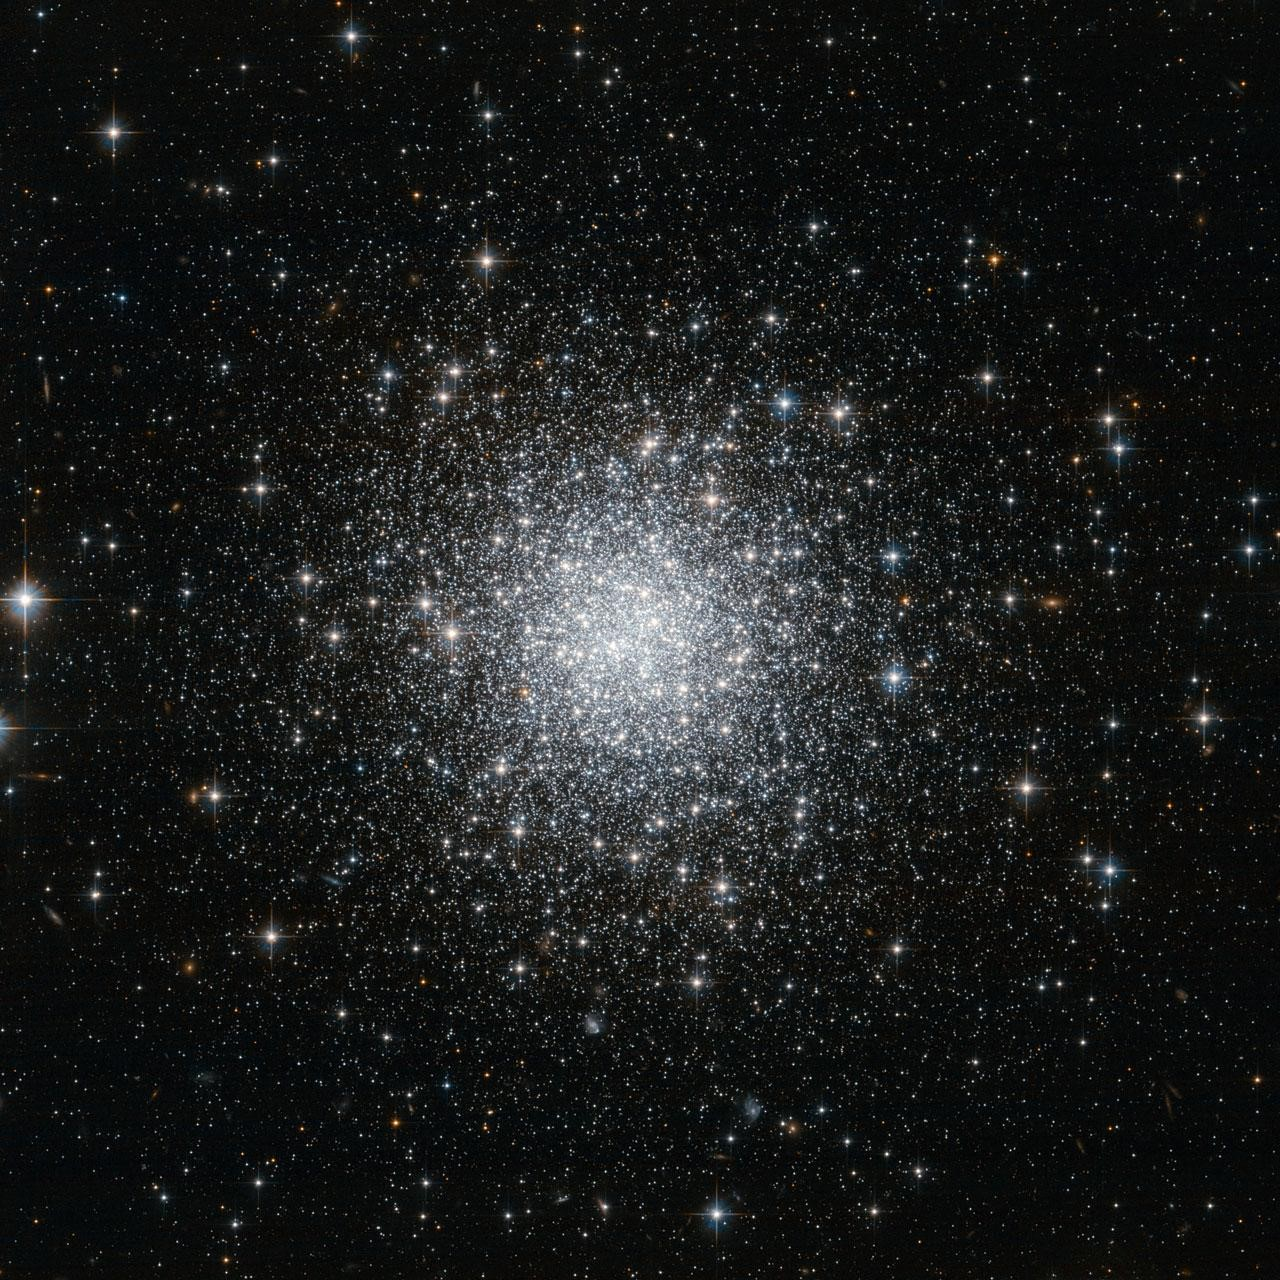
\includegraphics[width=0.8\textwidth]{figures/c42.jpg}
	\caption{The globular cluster NGC 7006 imaged by the Hubble Space Telescope's Advanced
		Camera for Surveys, photo courtesy of ESA/Hubble \& NASA}
	\label{fig:1/ngc7006}
\end{figure}



The study of stellar remnants in globular clusters has far-reaching implications for diverse fields
of astrophysics. Globular clusters are one of the most commonly proposed candidates to host
intermediate-mass black holes (IMBHs). Due to  the effects of mass segregation and the high
densities of the cores of globular clusters, the cores of globular cluster are an ideal environment
for mergers of compact objects. These mergers can be detected through their resultant gravitational
waves and the expected rates for gravitational wave events depend significantly on the compact
object populations in globular clusters. These mergers are also thought to be one of the most
promising formation channels for IMBHs, a so-far undetected class of black holes whose masses fall
between those of stellar mass black holes and those of supermassive black holes. The formation of
these black holes have important implications for understanding the formation of the supermassive
black holes that we find at the centre of galaxies.


This work builds on a previous project I worked on which used pulsar timing data to constrain the
properties of the globular cluster 47\,Tuc. In that work, we were able to place strong limits on the
mass in dark remnants (black holes, neutron stars, white dwarfs) within the cluster, establishing a
strong upper limit on the black hole content specifically. While this project was able to fully
account for effects like mass segregation and uncertain mass functions, one limitation of the models
that it used (which we will discuss in the following section) was the assumption that all objects
within the cluster are single. Because the masses of binary stars are higher than the typical masses
of objects within the cluster, they too will mass segregate to the core of the cluster like heavy
stellar remnants. While the binary fraction in 47\,Tuc is expected to be quite low
\citep{Milone2012}, the effects that a centrally concentrated population of binary stars might have
on the recovered remnant content of the cluster is still somewhat unclear and worth investigating.



\begin{figure}
	\centering
	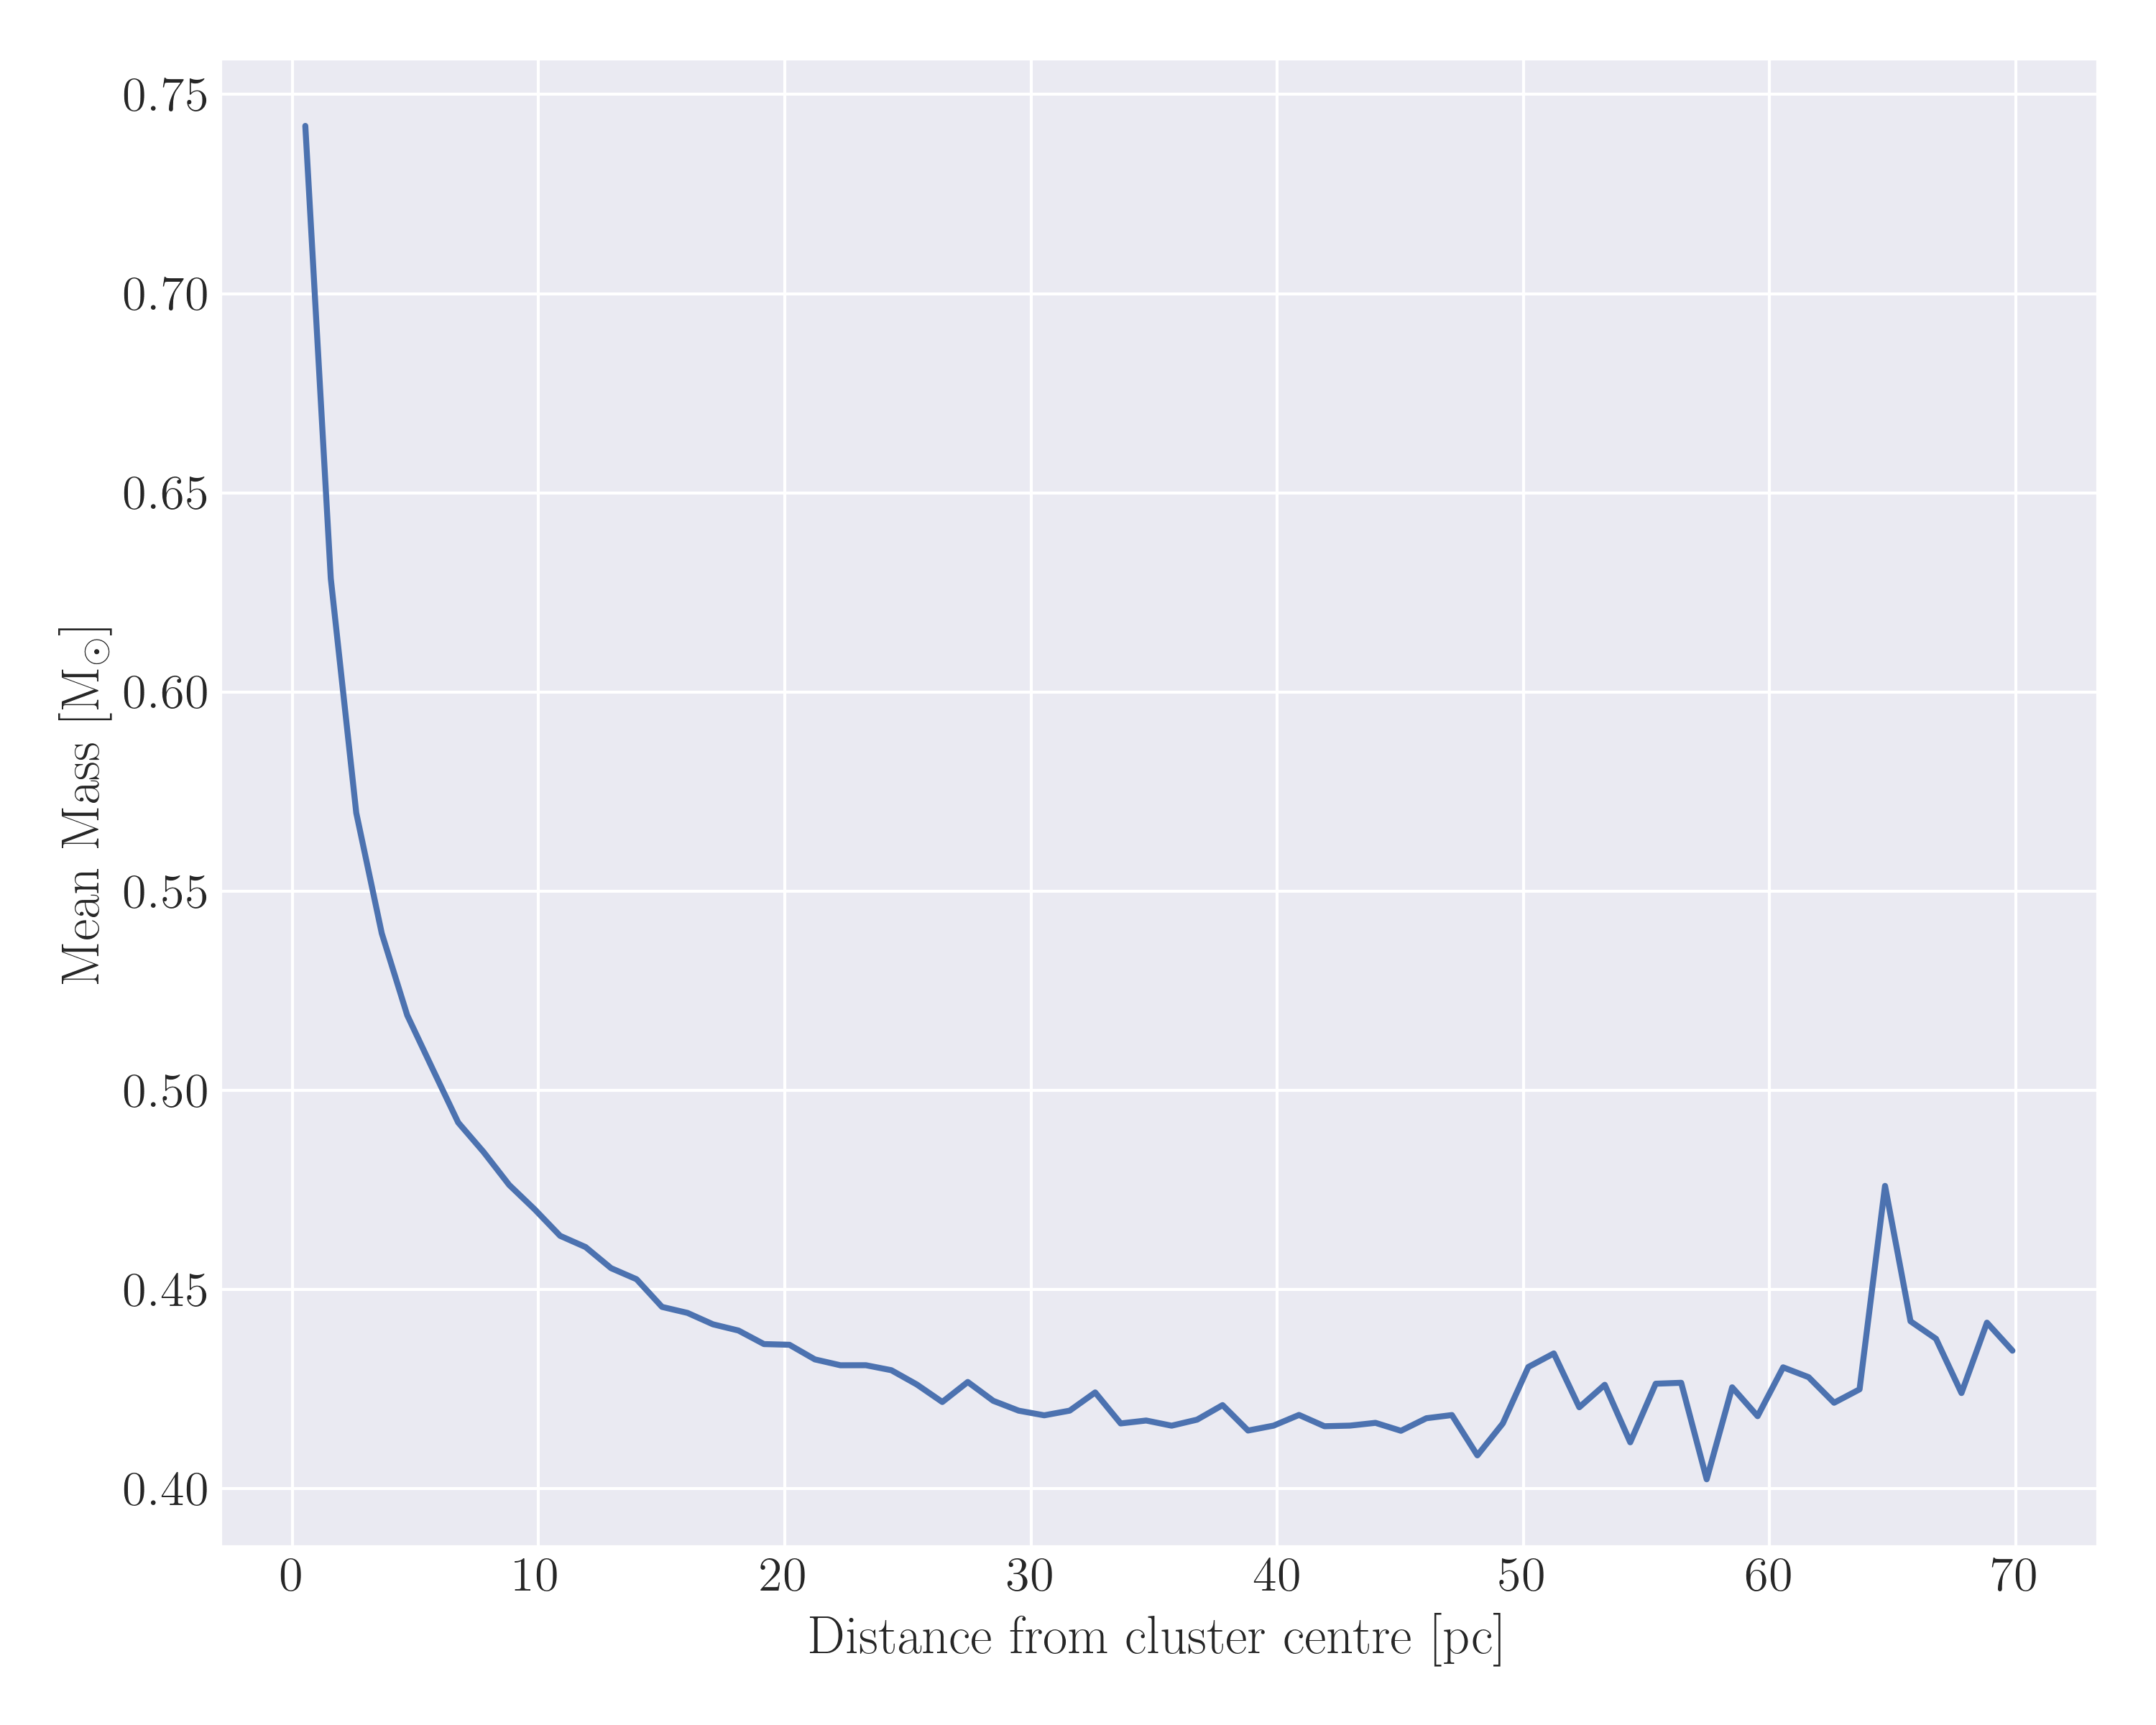
\includegraphics[width=0.8\textwidth]{figures/radial_mean_mass.png}
	\caption{Mean mass of objects within a realistic model of the globular cluster 47\,Tuc, as a
		function of radius. The concentration of high-mass objects in the central regions of
		the cluster is obvious, as is the preference for low-mas objects in the outskirts of
		the cluster.}
	\label{fig:1/radial_mean_mass}
\end{figure}




\section{Modelling Globular Clusters}

\paragraph{}

\ps{TODO: go through and make sure any jargon is properly explained}

When modelling globular clusters, there are generally two approaches commonly used. The first is to
model the entire evolutionary history of the cluster from initial conditions to the present-day. The
most commonly employed versions of these "evolutionary models" are direct N-body integration (see
for example \citet{Baumgardt2017a}) which directly calculate the gravitational interactions between
each object in the cluster and Monte-Carlo models (see \citet{Rodriguez2021} or \cite{Hypki2013})
which approximate the gravitational interactions between object according to the method of
\citet{Henon1971}. While these models provide insight into the dynamical history of the cluster,
they are very computationally expensive with even the fastest models taking on the order of a day to
model a realistic globular cluster \citep{Rodriguez2021}.

The second approach is to model just the present-day conditions of the cluster. These models, which
we call "equilibrium models", capture none of the dynamical history of the cluster but fully
describe the present-day state of the cluster. These equilibrium models are much less
computationally demanding than evolutionary models. Their relative efficiency allows us to explore a
significantly larger parameter space when fitting the models to observations to constrain the
present-day properties of a cluster. In particular, it is worth highlighting that by using
equilibrium models we are able to vary the stellar mass function of the cluster as well as the black
hole and remnant retention fractions with more flexibility than what might be possible with
evolutionary models, due to the computational cost of computing extensive grids of evolutionary
models with many parameters varied in the initial conditions (e.g. various stellar initial mass
functions, initial cluster radii, masses, etc.).

The comparative efficiency of these models further enables the use of statistical fitting techniques
like MCMC or Nested Sampling which would be prohibitively expensive to use with evolutionary models.
This means that instead of a computing a grid of models and finding the "best-fitting" model we can
instead recover posterior distributions for key cluster parameters.


In this work we use the \code{LIMEPY} family of models presented by \citet{Gieles2015}. The
\code{LIMEPY} models are a set of distribution function based equilibrium models that are isothermal
for the most bound stars near the cluster centre and described by polytropes in the outer regions
near the escape energy. The models have been extensively tested against $N$-body models
\citep{Zocchi2016, Peuten2017} and are able to effectively reproduce the effects of mass
segregation. Their suitability for mass modelling globular clusters has been tested on mock data
\citep{Henault-Brunet2019} and they have recently been applied to real datasets as well
\citep[e.g.][]{Gieles2018, Henault-Brunet2020}.


\begin{figure}
	\centering
	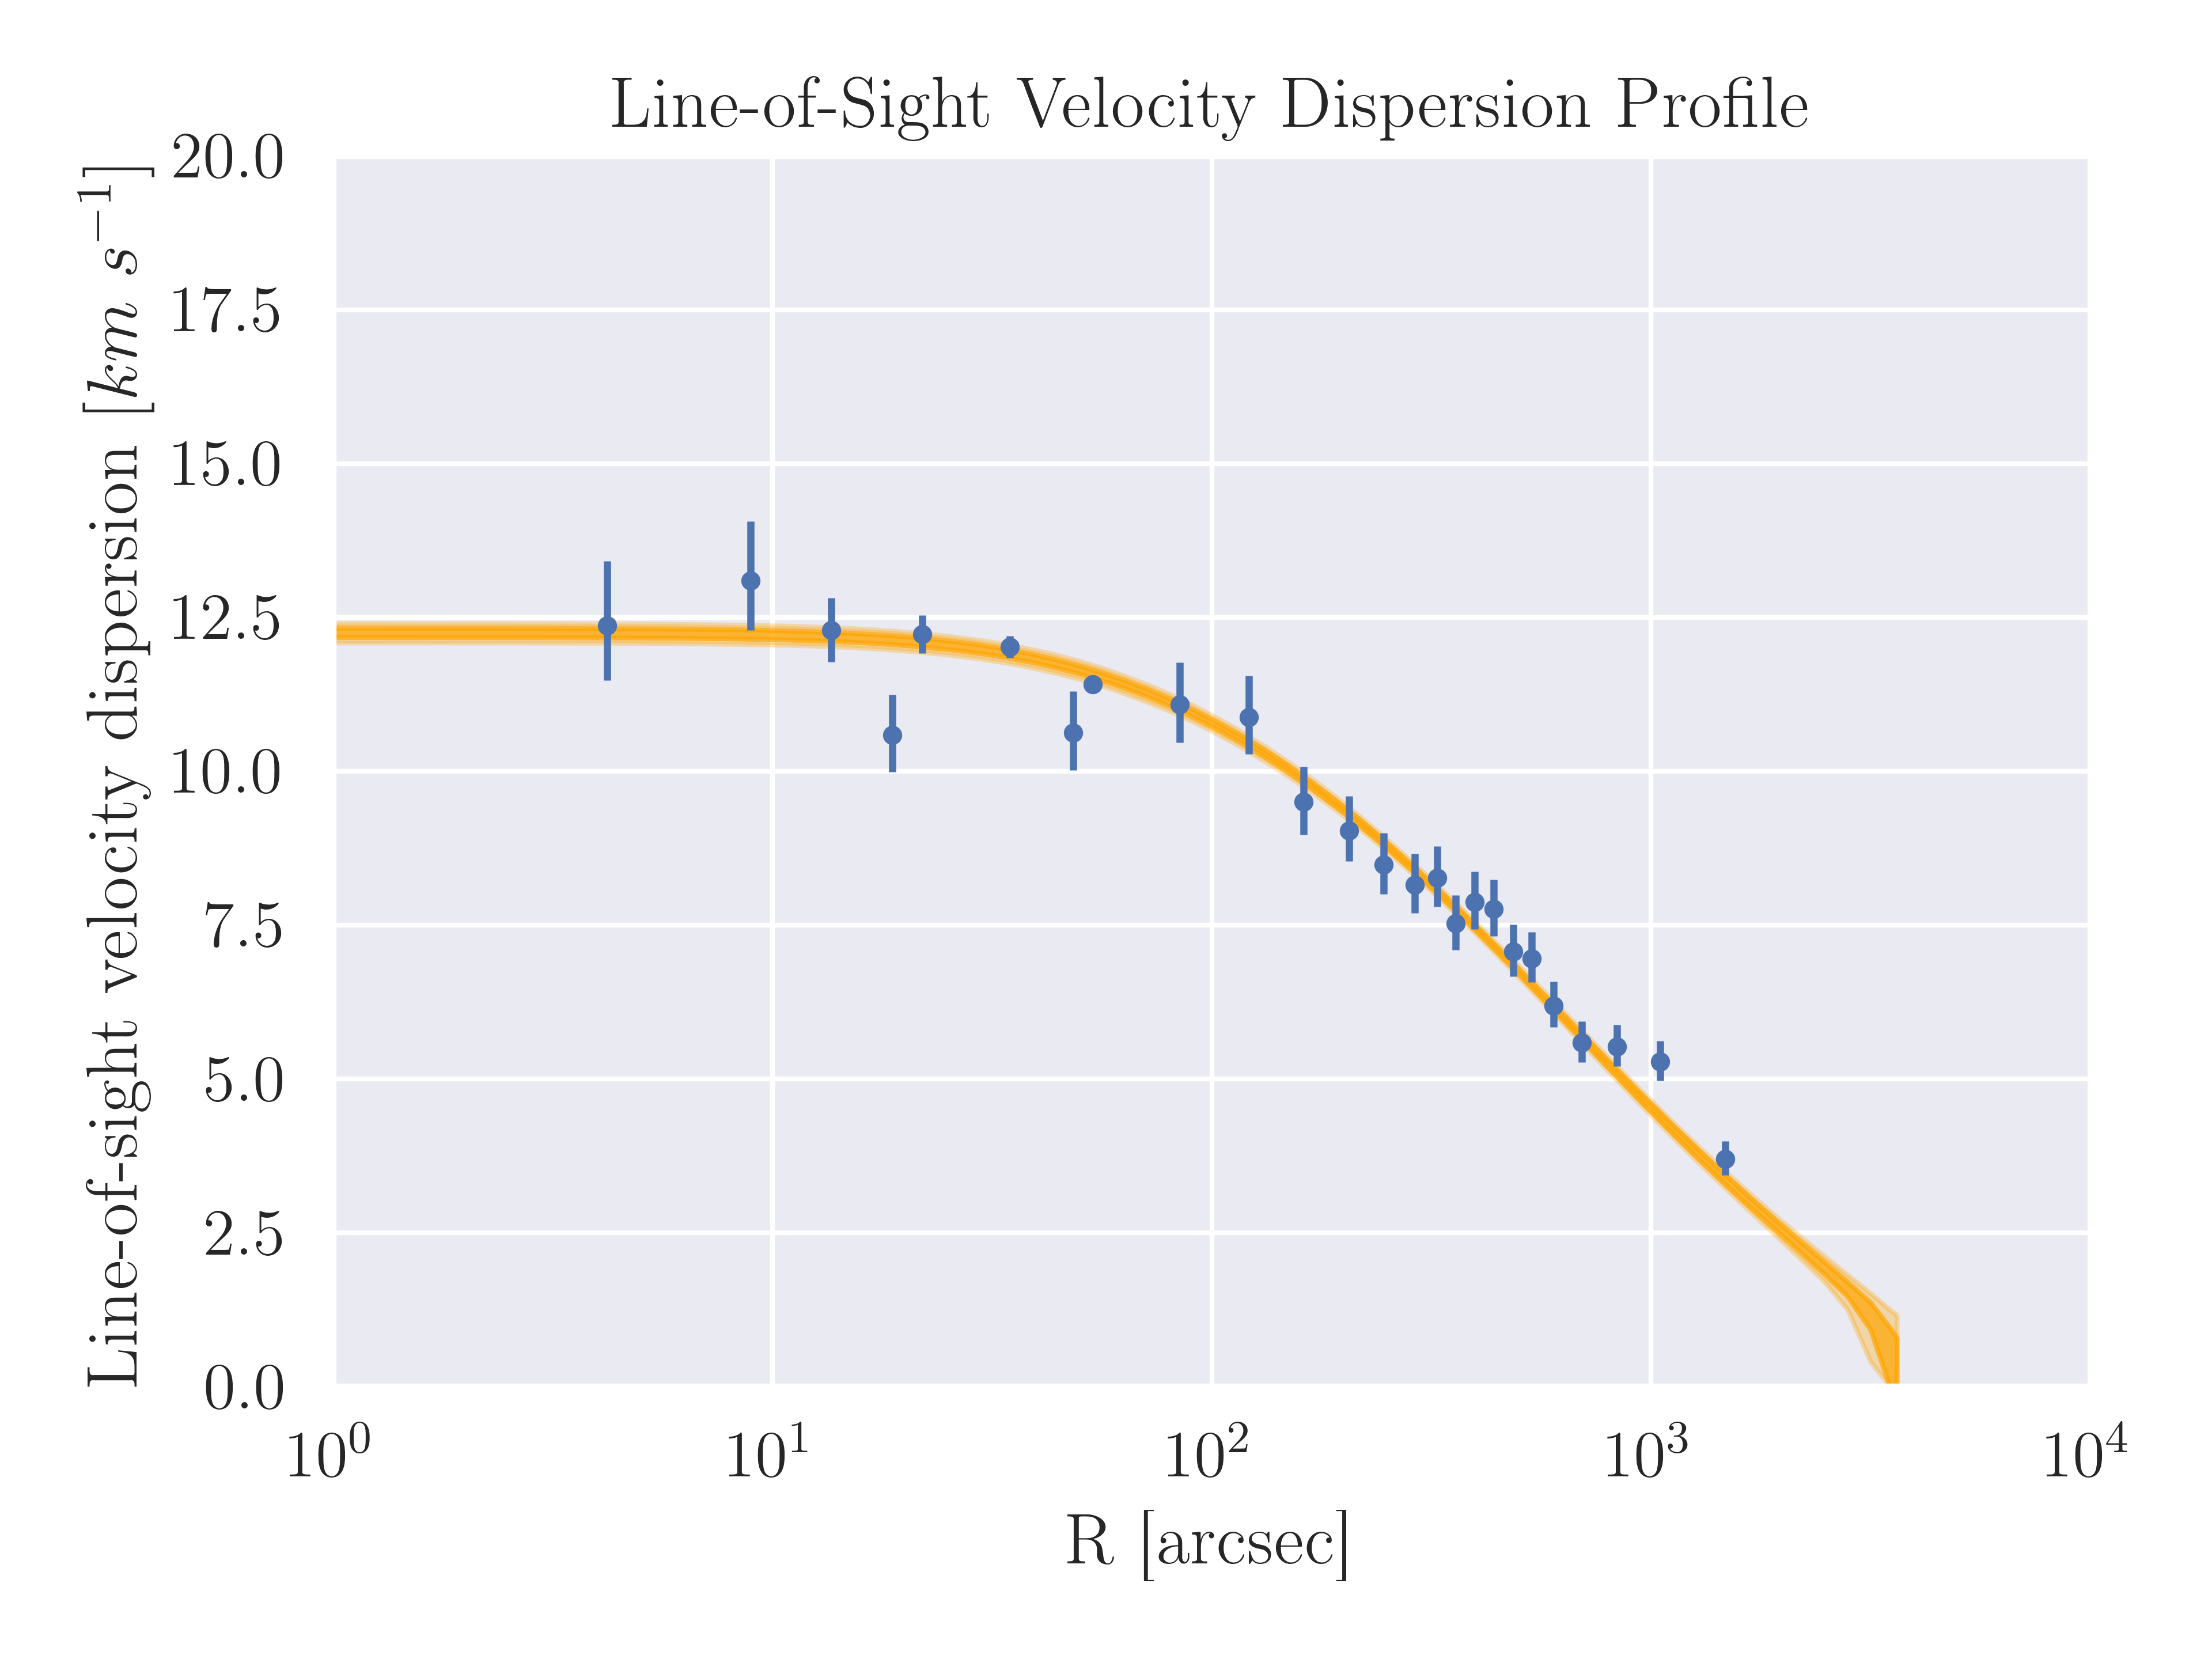
\includegraphics[width=0.8\textwidth]{"./figures/limepy_veldisp.png"}
	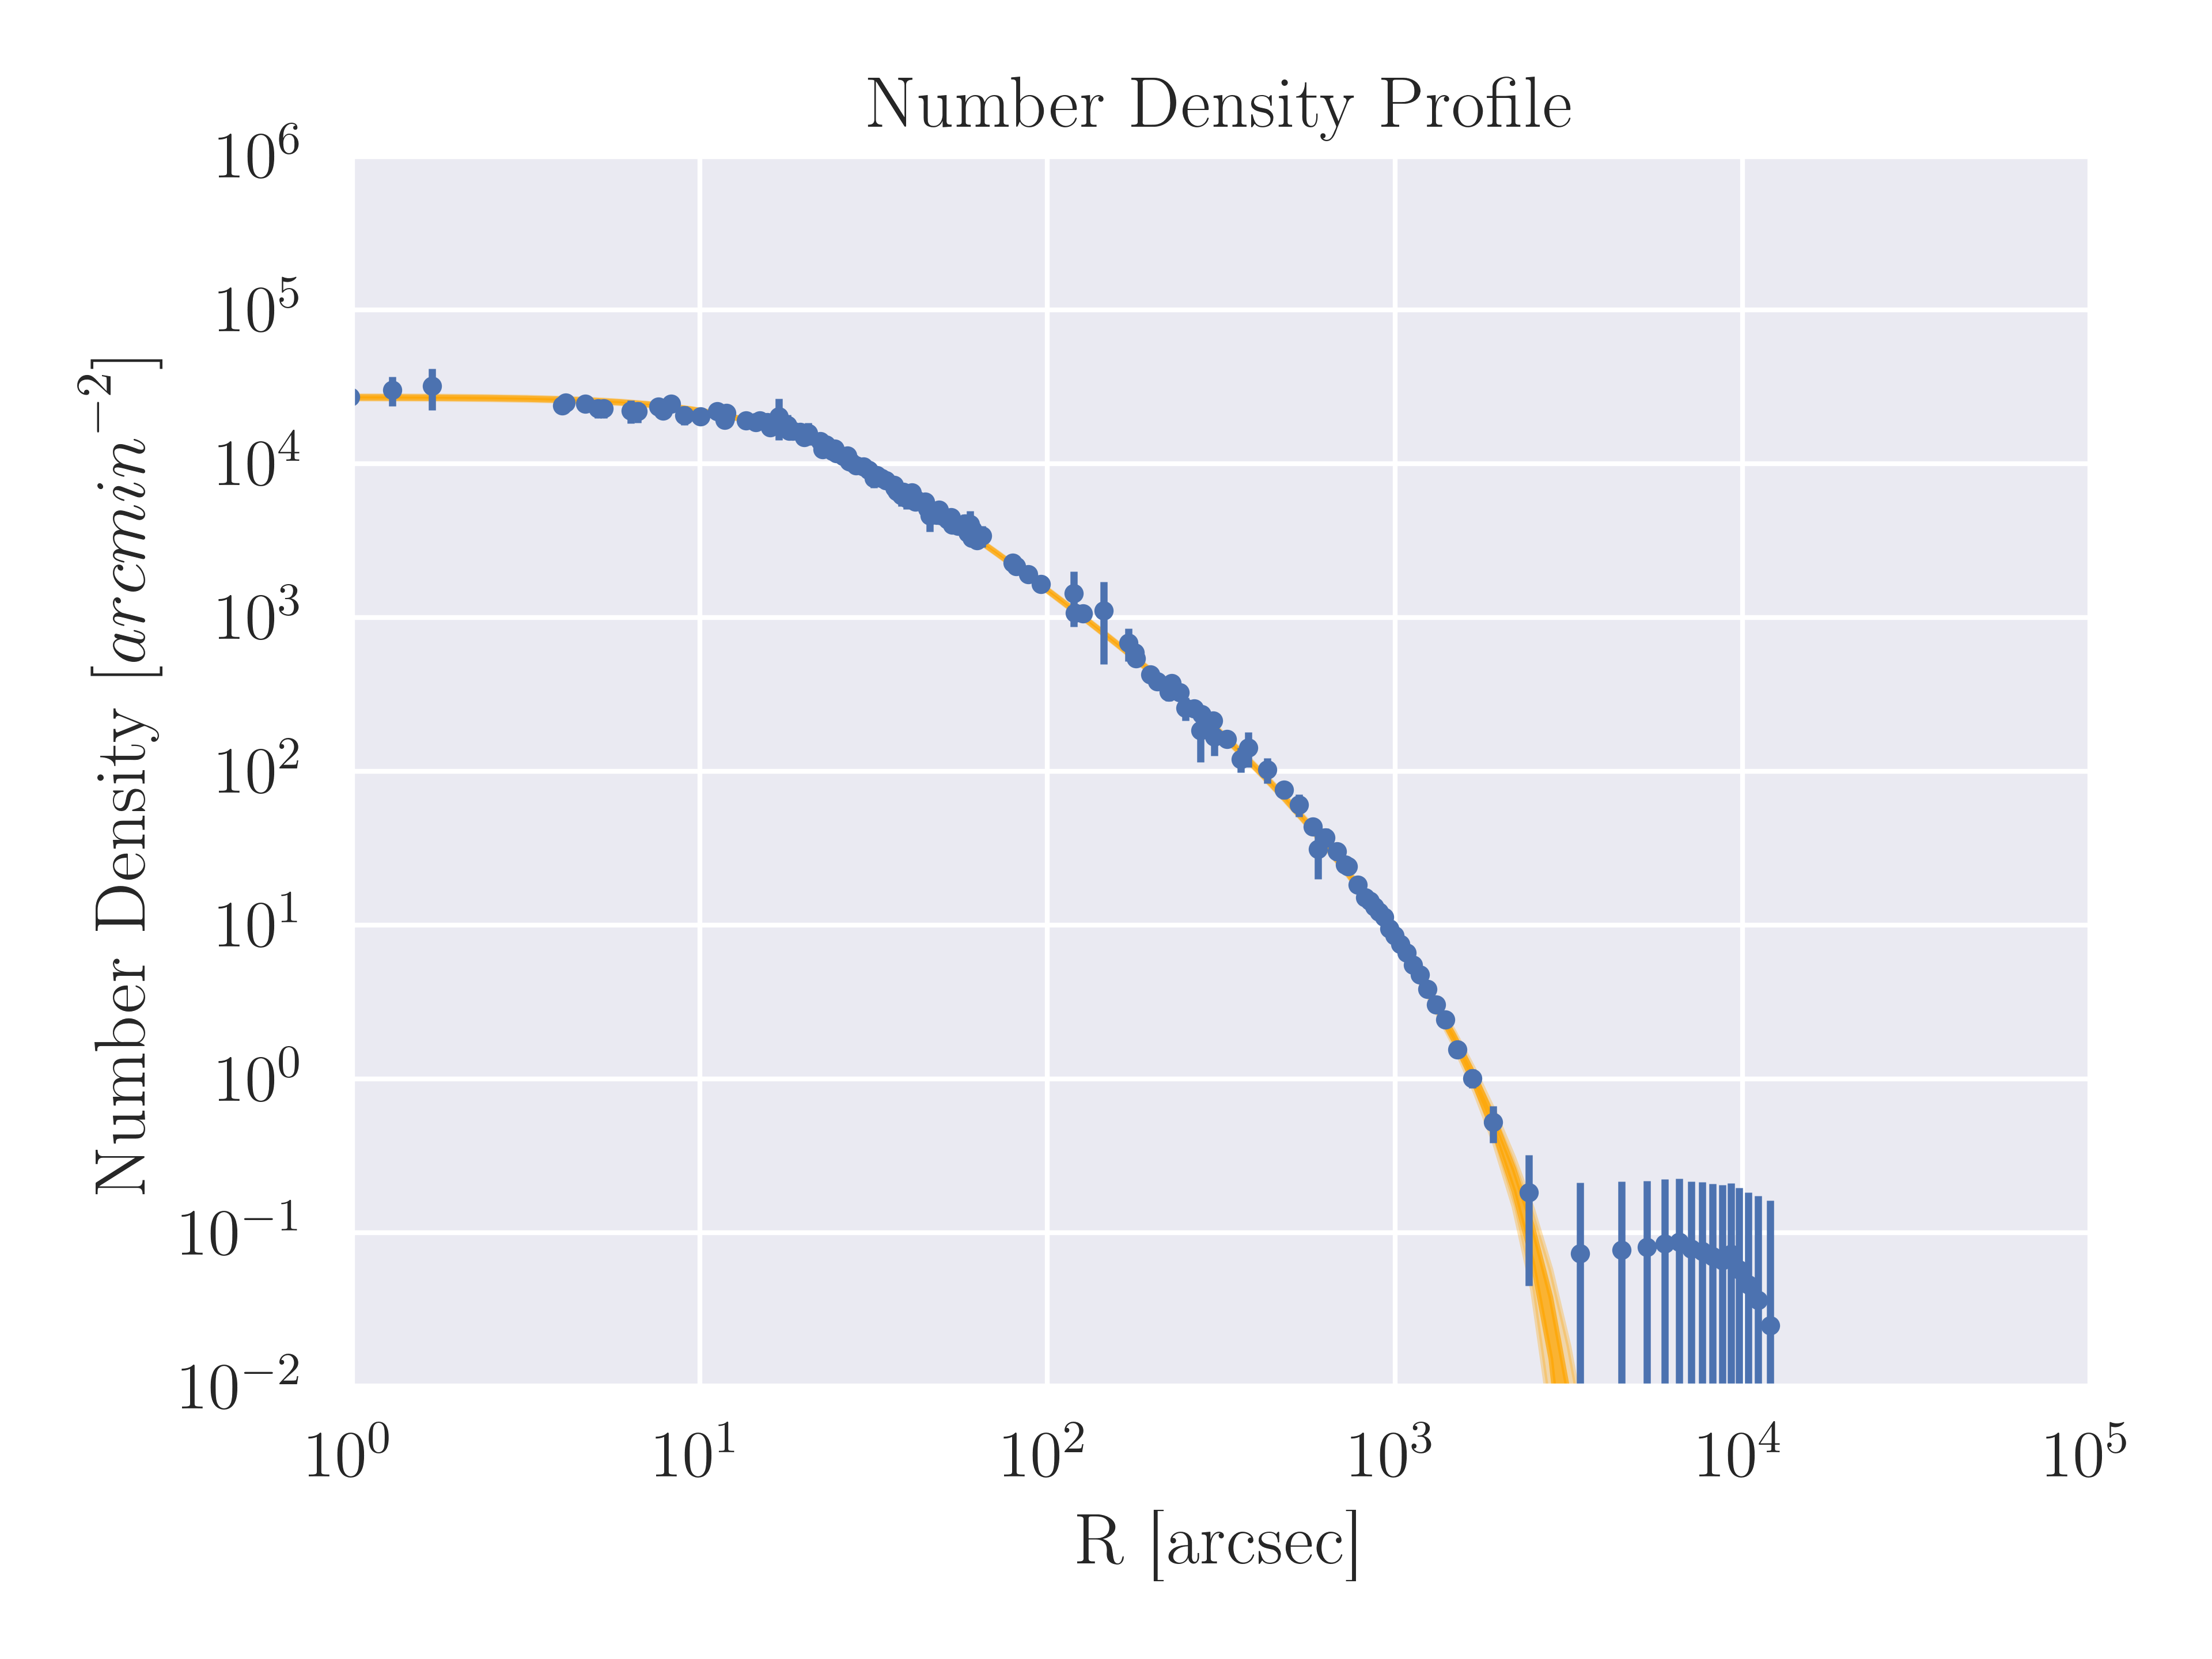
\includegraphics[width=0.8\textwidth]{"./figures/limepy_numdens.png"}
	\label{fig:1/limepy_models}
	\caption{\ps{TODO: write proper caption} Some fits of limepy models to 47 Tuc}
\end{figure}


The input parameters needed to compute our models include the central concentration parameter $W_0$,
the truncation parameter $g$\footnote{Woolley models \citep{Woolley1954} have $g=0$, King models
	\citep{King1966} $g=1$, and Wilson models \citep{Wilson1975} $g=2$.}, the anisotropy radius $r_a$
which determines the degree of radial anisotropy in the models, $\delta$ which sets the mass
dependence of the velocity scale and thus governs the degree of mass segregation, and finally the
specific mass bins to use as defined by the mean stellar mass ($m_j$) and total mass ($M_j$) of each
bin, which together specify the stellar mass function. In order to scale the model units into
physical units, the total mass of the cluster $M$ and a size scale (the half-mass radius of the
cluster $r_h$) are provided as well.


In their current implementation, these models assume that all objects within the cluster are single
and make no attempt to model the dynamical effects of stellar multiplicity. In this project we adapt
these models to incorporate some of the effects of binary stars under the assumption that all
long-period binaries have been ionized by the present-day. This allows us to treat binary systems as
point-masses and lets us model their dynamics by simply moving some of the mass in stars into
heavier bins according to the specified binary population.



\section{Binary Stars}
\subsection{Binaries in Globular Clusters}

\ps{Discuss binaries in general, mention terminology, then why binaries in clusters are different
	from field binaries, then the dynamical effects of binaries}

In general, the binary systems found within present-day clusters differ significantly from the field
binaries that are more easily observed. In particular, we expect to little no long-period binaries,
on account of them being ionized by the frequent interactions with other cluster members. We
frequently use the terms "hard" and "soft" to describe binaries where "soft binaries" have a binding
energy comparable to the average kinetic energy of a cluster member while "hard binaries" have
larger binding energy. Due to the frequent interactions within clusters we expect that all soft
binaries have long since been ionized by the present-day leaving only a population of hard binaries
with a truncated period distribution compared to field binaries.
\ps{Cite some papers here}

% Binary Burning: \citet{Chatterjee2013}


% Black Hole Burning: \citet{Kremer2019}



The most obvious way that binaries can effect the dynamics of a cluster is through three-body
interactions with other cluster members. When a single star (or another binary) interacts with a
binary system at a close enough range, the binary system will either impart some of its energy to
the ejected star and "harden" or it will capture the approaching star, while ejecting one of its
original components, forming a "harder" binary \citep{Heggie2003}. In either of these cases the
binary system will impart some extra kinetic energy to the ejected star, through this process binary
systems can act as a reserve of kinetic energy for a cluster and are thought to be one of the
primary mechanisms through which core-collapse is halted in some clusters \citep{Chatterjee2013}.
Because the models that we will be focusing on do not model individual objects within the cluster we
will instead focus of the second way that binaries can effect the dynamics of a cluster.

Because binaries are tightly bound, for all interactions except for the very closest, they
effectively act as a single point mass equal to the sum of each component's mass. In this way,
binaries can affect cluster dynamics in much the same way that a large population of heavy remnants
might. Much like black holes and neutron stars, binary systems will migrate to the centre of a
cluster due to the effect of mass-segregation. \citet{Kremer2019} found that a central population of
black holes can fulfill a similar role to binary systems in halting core collapse by injecting
kinetic energy through two-body interactions within the core of the cluster. This same mechanism
could apply with tightly-bound binary systems that have mass-segregated to the centre of the
cluster. This predicted increase in binary fraction as you get closer to the centre of a cluster is
also seen in observations, and is illustrated in Figure \ref{fig:1/radial_binary_fraction} for NGC
3201.

The effect of having a large central population of binaries could be that our models are
overestimating the amount of mass needed in dark mark and therefore overestimating the number of
black holes and high-mass objects in general. Because the gravitational potential in the central
regions is fairly well constrained by kinematic measurements, if we are missing a significant
contribution from binaries, the models may be compensating for this "missing mass" by adding more
mass to the heavy end of the IMF which would lead to overestimation of the number of neutron stars
and black holes.




\begin{figure}
	\centering
	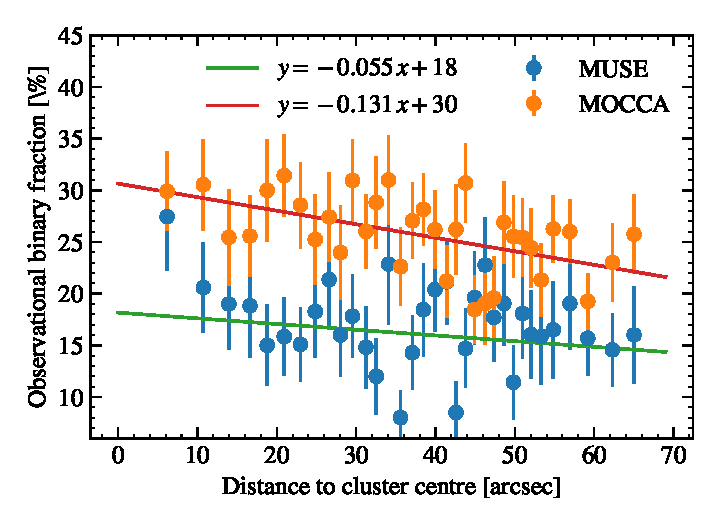
\includegraphics[width=0.8\textwidth]{figures/radial_binarity.pdf}
	\caption{Reproduced from Figure 8 of \citet{Giesers2019} \ps{TODO: Caption, mention what MOCCA is}}
	\label{fig:1/radial_binary_fraction}
\end{figure}

\subsection{Observations of Binary Stars in Globular Clusters}

\paragraph{}
In general, there are two methods used to detect binaries within globular clusters: high-precision
photometric observations and radial velocity surveys.

\paragraph{}
High-precision photometry can be used to detect binaries along the main sequence which have a
significant difference in the mass of their components ( typically these systems have a mass ratio,
$q$, larger than $0.5$). These systems will appear to be raised above the main-sequence when plotted
on a colour-magnitude diagram as their colour will match that of a typical main-sequence star
however their luminosity will be the sum of both components. Figure
\ref{fig:1/main_sequence_binaries} shows the main-sequence of the cluster NGC 2298, the binary stars
in this cluster are visible above the main-sequence according to their mass ratio.
\citet{Milone2012} performed high-precision photometry on several globular clusters using the Hubble
Space Telescope's (HST) Advanced Camera for Surveys and was able to place strong constraints on the
binary fraction for binaries with a mass ratio above $q=0.5$. This method allows for large studies
of binary populations in GCs without the need for dedicated observations but suffers from an
inherent bias towards systems with high mass ratios. Systems with mass ratios below $q=0.5$ are
typically too close to the regular main-sequence to confidently classify as binaries (see Figure
\ref{fig:1/main_sequence_binaries}). This means that studies which employ this method must assume an
underlying mass-ratio distribution if they wish to place any limits on the overall binary fraction
of a cluster.


\begin{figure}
	\centering
	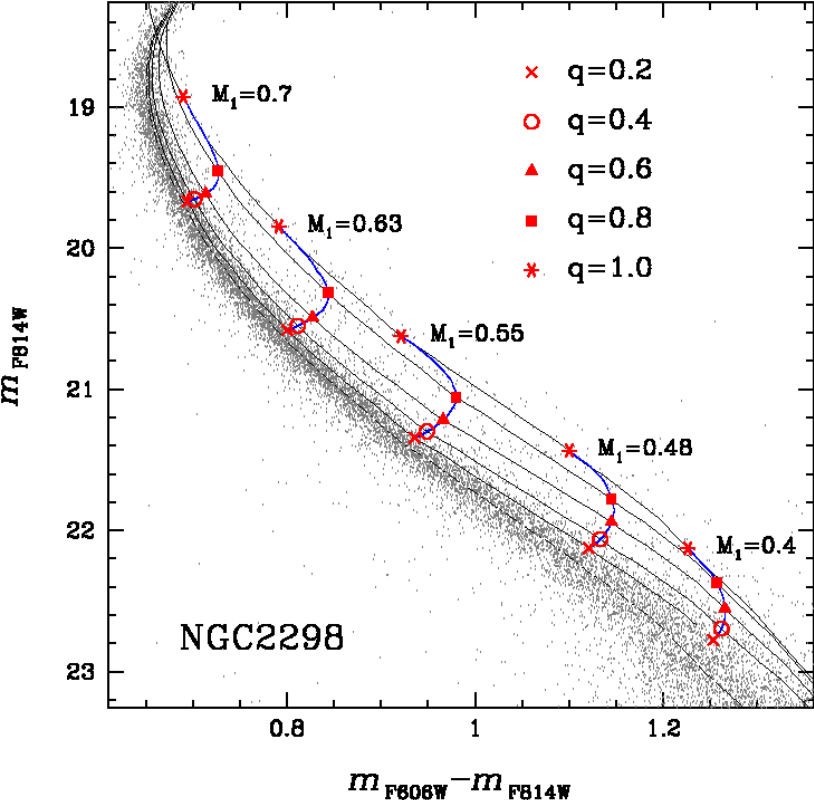
\includegraphics[width=0.8\textwidth]{"./figures/main_sequence_binaries.pdf"}
	\label{fig:1/main_sequence_binaries}
	\caption{\ps{TODO: write proper caption} Reproduced from Figure 1 of \citet{Milone2012}.}
\end{figure}


Large-scale campaigns to measure the radial velocities for many stars in a cluster over many epochs
are another method which can be used to detect binaries in GCs. Systems which are found to have
periodically varying radial velocities can typically be confidently classified as binary systems.
\citet{Giesers2019} used the MUSE integral field spectrograph installed at the European Southern
Observatory's Very Large Telescope to observe several GCs and reported the results for NGC 3201.
Integral field spectrographs provide spatially resolved spectra for the entire field of view of the
detector which enables far more time-efficient surveys than previous methods. Because this method
measures radial velocities over time, periods for the binaries can be accurately determined and
given enough measurements, many other parameters like eccentricity and companion mass can be
accurately constrained in contrast to photometric methods which can only provide the mass ratio.


\newpage

\chapter{Methods}
\newcommand{\evolvemf}{\code{evolve\_mf}}



\section{Data}


We use a wide range of data to constrain the parameters of our models. In general, we use archival
kinematic data from ground based spectroscopy, number density profiles from \emph{Gaia}, stellar
mass function data from HST photometry and pulsar timing data.

\subsection{Kinematics and density profiles}

\subsubsection{Proper motion dispersion profiles}

We use two sets of {\it Hubble Space Telescope} (HST) proper motion data. To probe the inner regions
of the cluster we use the proper motion dispersion profiles (both tangential and radial components)
from \citet{Watkins2015} which are based on a catalogue of proper motions of bright stars from
\citet{Bellini2014}. These dispersion profiles are built from stars brighter than the main sequence
turn-off (around $0.85 \ \mathrm{M}_\odot$  for 47\,Tuc). To probe the kinematics in the outer
regions of the cluster, we also use the data from \citet{Heyl2017}, for which the mean mass of the
measured stars is $0.38 \ \mathrm{M}_{\odot}$. The outer proper motion data also allows us to
constrain the amount of radial anisotropy present in the cluster, which can mimic the effect of
central dark mass in isotropic models by raising the central velocity dispersion \citep{Zocchi2017}.


\subsubsection{Line-of-sight velocity dispersion profiles}

We use the line-of-sight velocity dispersion profile from \citet{Baumgardt2018} to further constrain
the kinematics of the cluster. The dispersion profile is based on archival ESO/VLT and Keck spectra
along with previously published radial velocity data from the literature. As these radial velocity
samples are dominated by bright stars, we assume that the velocity dispersion profile traces the
kinematics of upper main-sequence and evolved stars in our models.

\subsubsection{Number density profiles}
We use the number density profile from \citet{DeBoer2019} to constrain the size and structural
parameters of the cluster. These profiles are made up of a combination of cluster members based on
Gaia DR2 data in the outer regions and data from various literature sources in the central regions.
The Gaia data used only includes bright stars ($m > 0.6 \ \mathrm{M}_\odot$, for both clusters) and
the literature data is dominated by bright stars, therefore in our models we assume the profiles
probe the distribution of upper main sequence and evolved stars.

\subsection{Stellar mass functions}

As a constraint on the global present-day stellar mass function of the cluster, we use a compilation
of HST based stellar mass function data from
Baumgardt\footnote{\url{https://people.smp.uq.edu.au/HolgerBaumgardt/globular/}} (2021, priv.
comm.), which represent an updated and augmented version of the stellar mass functions found in
\citet{Sollima2017}. This compilation is made up of several HST fields at varying distances from the
cluster centre. These fields extend out to $14 '$ from the cluster centres for 47\,Tuc and cover a
mass range of $0.16 - 0.8 \ \mathrm{M}_\odot$. The large radial and mass ranges allow us to
constrain the degree mass segregation in the clusters.

\subsection{Pulsar Data}

For 47\,Tuc, we make use of its large population of millisecond pulsars (MSPs) to place further
constraints on its mass distribution. We use both the spin and orbital period timing solutions from
\citet{Freire2017}, \citet{Ridolfi2016} and \citet{Freire2018}. We also consider the dispersion
measures of the pulsars which, when combined with internal gas models from \citet{Abbate2018}, allow
us to constrain the line-of-sight position of the pulsars within the cluster. The work surrounding
the use of pulsar data to constrain the models was performed as part of an earlier project and so
will not be discussed in too much detail in this project.



\subsection{Binary Data}

In order to create realistic binary populations we use the data from \citet{Milone2012} to inform
our choices of binary fraction and mass ratio distribution. For 47\,Tuc this means a flat mass
ration distribution and a binary fraction of roughly $2\%$. Because this estimate of the binary
fraction is so small, we will use it as a lower limit for the binary fraction and also test a case
where the binary fraction is around $10\%$ representing a case where the binary fraction is quite
significant.




\section{Generating mass functions}

The bulk of project deals with generating mass functions to use as inputs to the \code{LIMEPY}
models, we do this in two main steps, we first generate a present-day mass function comprised of
only single stars, and we then modify it to include binary stars.

\subsection{Single Star Mass Functions}


To generate the mass functions comprised of single stars we use the \evolvemf{} algorithm from
\code{SSPTools}\footnote{\url{www.github.com/pjs902/ssptools}} (first presented in
\citealt{Balbinot2018}), a publicly available package for working with simple stellar populations.

The \evolvemf{} algorithm combines precomputed grids of stellar evolution models and isochrones to
accurately model the evolution of a given initial mass function, fully including the effects of
stellar evolution as well as mass loss due to escaping stars and dynamical ejections. The algorithm
returns a sampled mass function at a requested evolutionary time, ideal for use in the \code{LIMEPY}
models.

We parameterize the mass function as a broken power-law with breakpoints at $0.5 \mathrm{M}_\odot$
and $1.0 \mathrm{M}_\odot$. We provide to \evolvemf{} the initial mass function slopes and
breakpoints, the cluster age, metallicity and escape velocity, as well as parameters which control
the mass loss due to escaping stars and the specific binning to be used when the present day mass
function is sampled. Figure \ref{fig:2/evolve_mf} shows the evolution of a mass function over a span
of $10 \ \mathrm{Gyr}$.

\begin{figure}
    \centering
    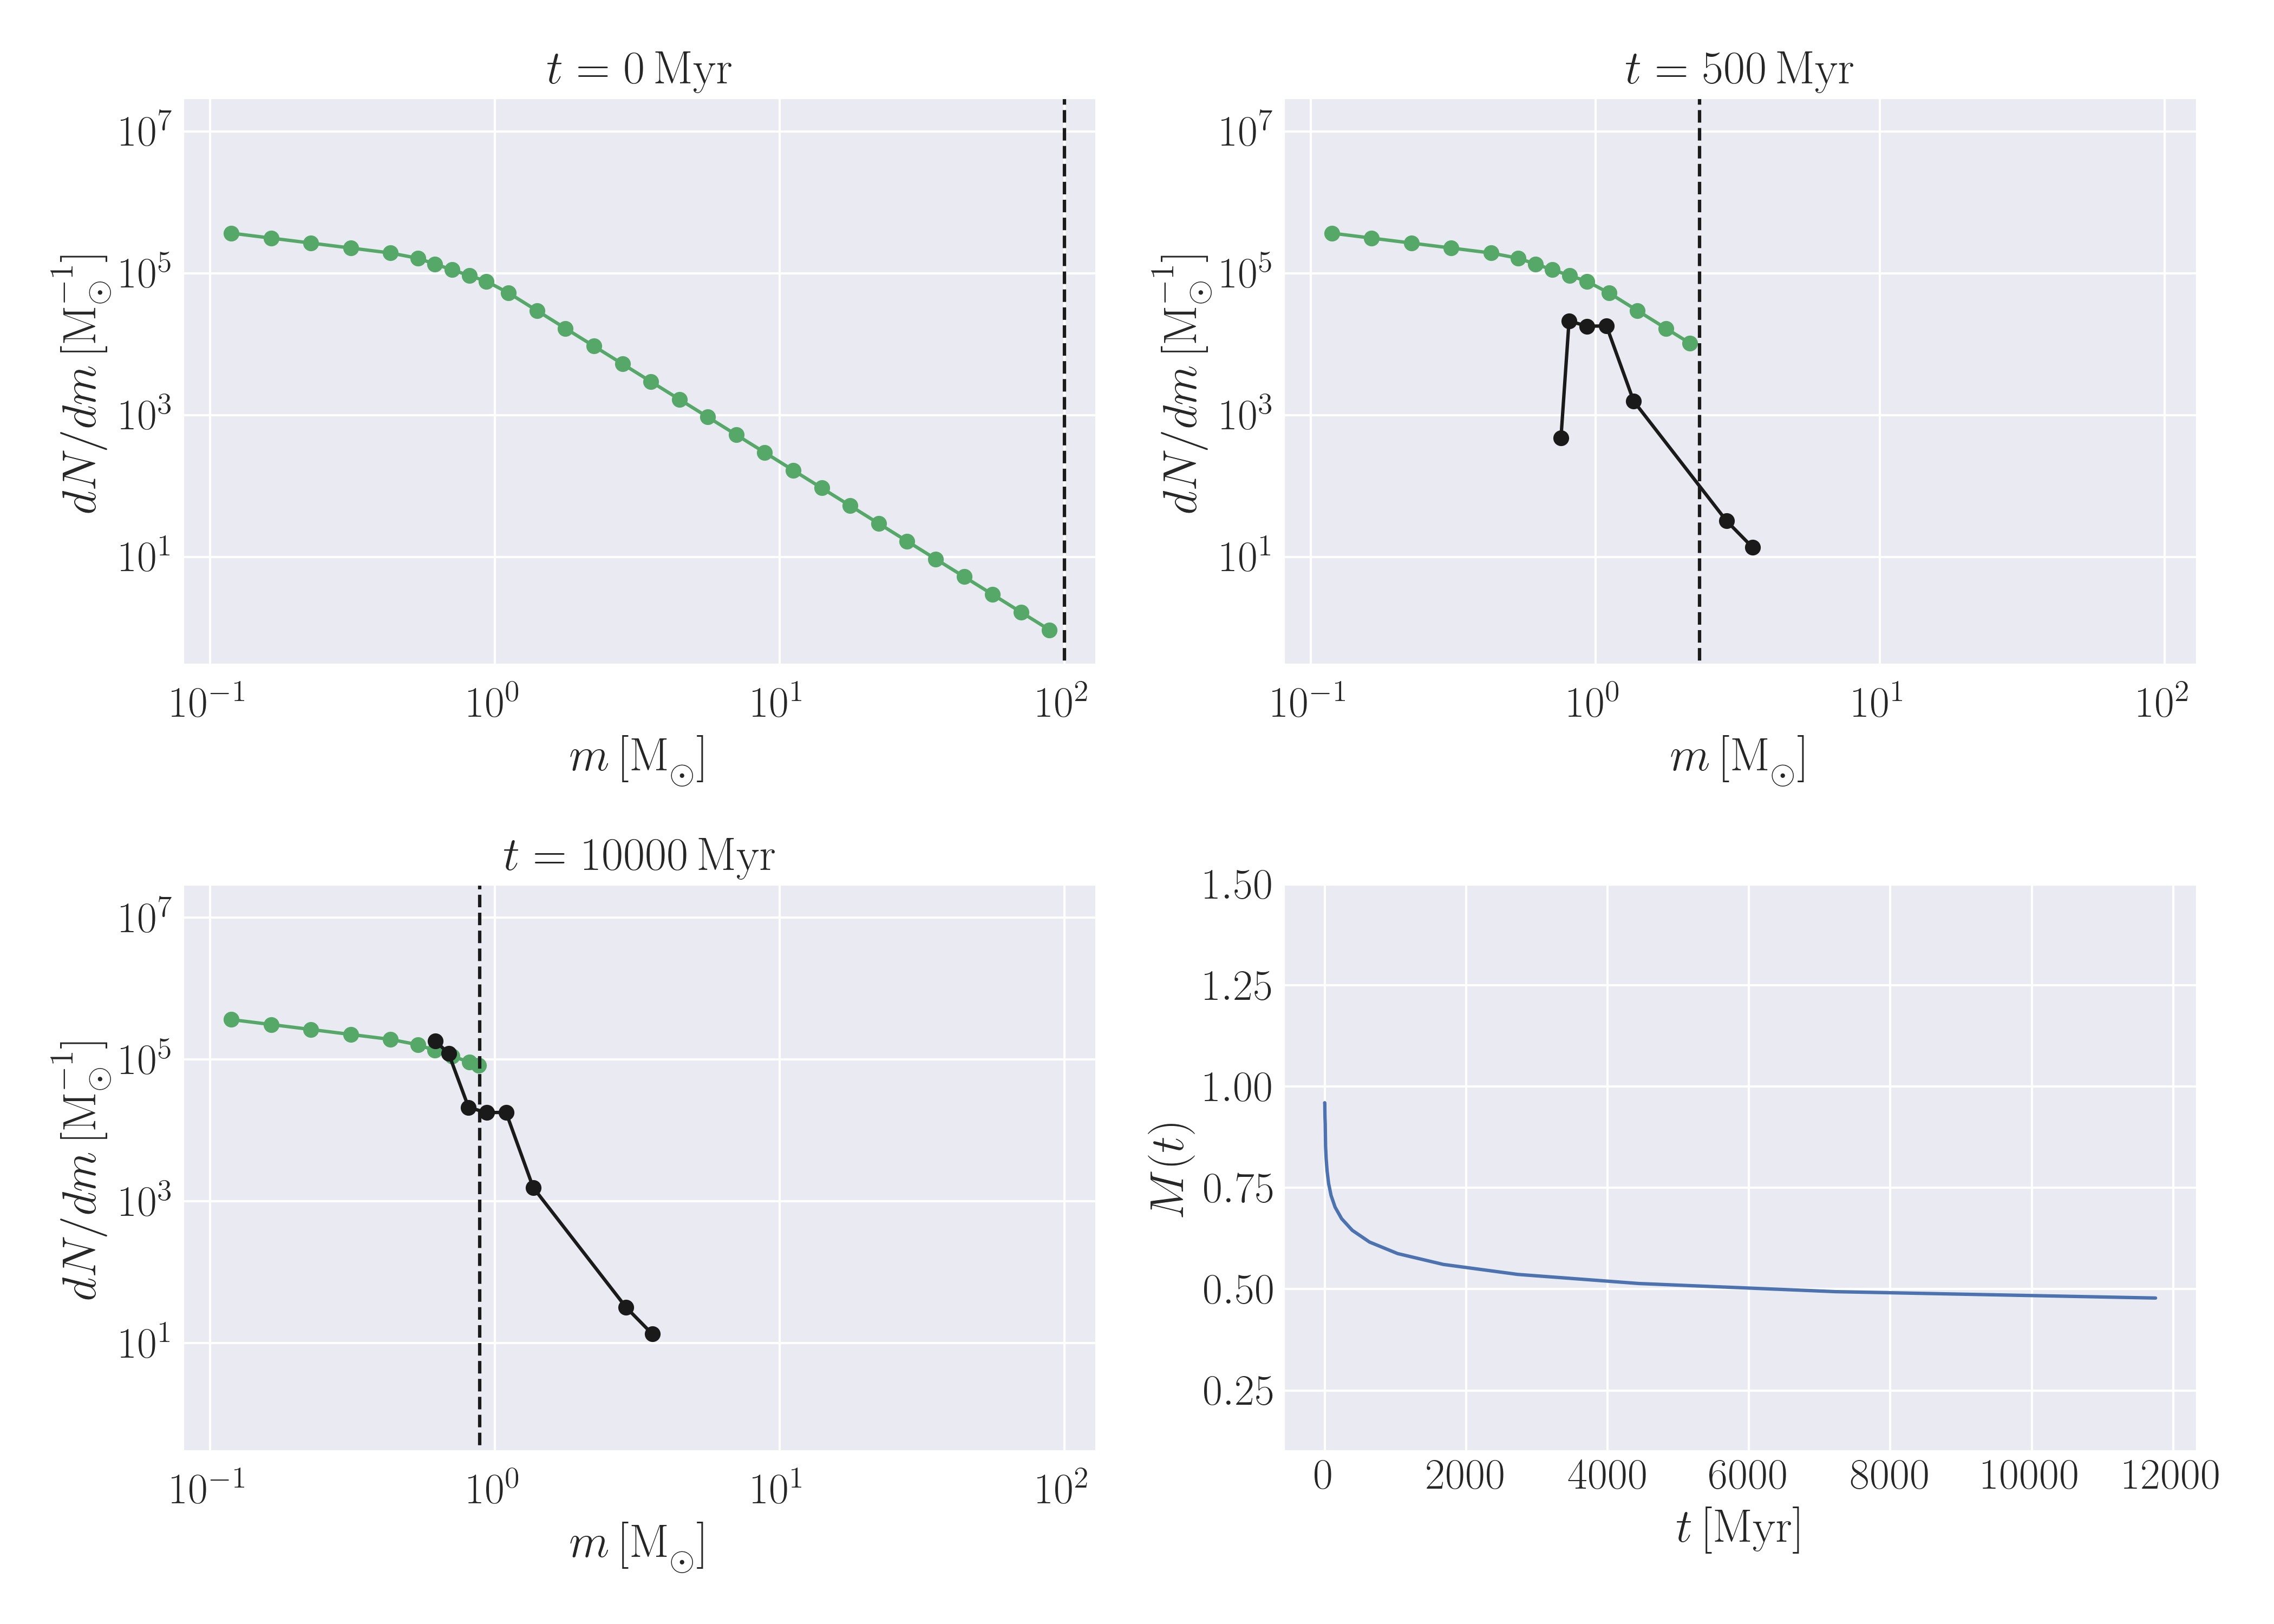
\includegraphics[width=\textwidth]{figures/evolve_mf.png}
    \caption{The evolution of a typical mass function from $t=0$ to $t=10000 \ \mathrm{Myr}$. The
        stellar bins are plotted in green while the remnant bins are plotted in black, the current
        main-sequence turn-off is plotted as a dashed black line. As the mass function ages, more
        and more main sequence stars evolve into remnants. Lower right: The evolution of the total
        mass of the mass function is plotted as a fraction of the initial mass. Mass loss is
        dominated by the effects of stellar evolution but also has contributions from dynamically
        ejected and escaping stars.}
    \label{fig:2/evolve_mf}
\end{figure}


\subsection{Binary Mass Functions}

In order to include binary stars in our mass functions we make use of the assumption that for the
vast majority of their interactions with other objects, binary systems behave essentially as point
masses due to the fact that they are tightly bound. This means that in order to replicate the
effects of a binary population in our mass function, we simply need to shift some of the mass in
single stars into heavier bins which act as the "binary bins".


We split this process up into several steps. First we divide the total binary fraction among the
values of $q$ in the requested mass ratio distribution. We weight the $f_b$ values assigned to the
individual values of $q$ by the chosen mass ration distribution, a flat mass ratio distribution
would have the total binary fraction divided evenly among the values while a "solar distribution"
(see \citealt{Fisher2005}) would have a significantly higher portion of the total $f_b$ assigned to
equal mass binaries ($q=1$). Figure \ref{fig:2/q-dists} shows the resulting mass ratio distributions
using this method.

\begin{figure}
    \centering
    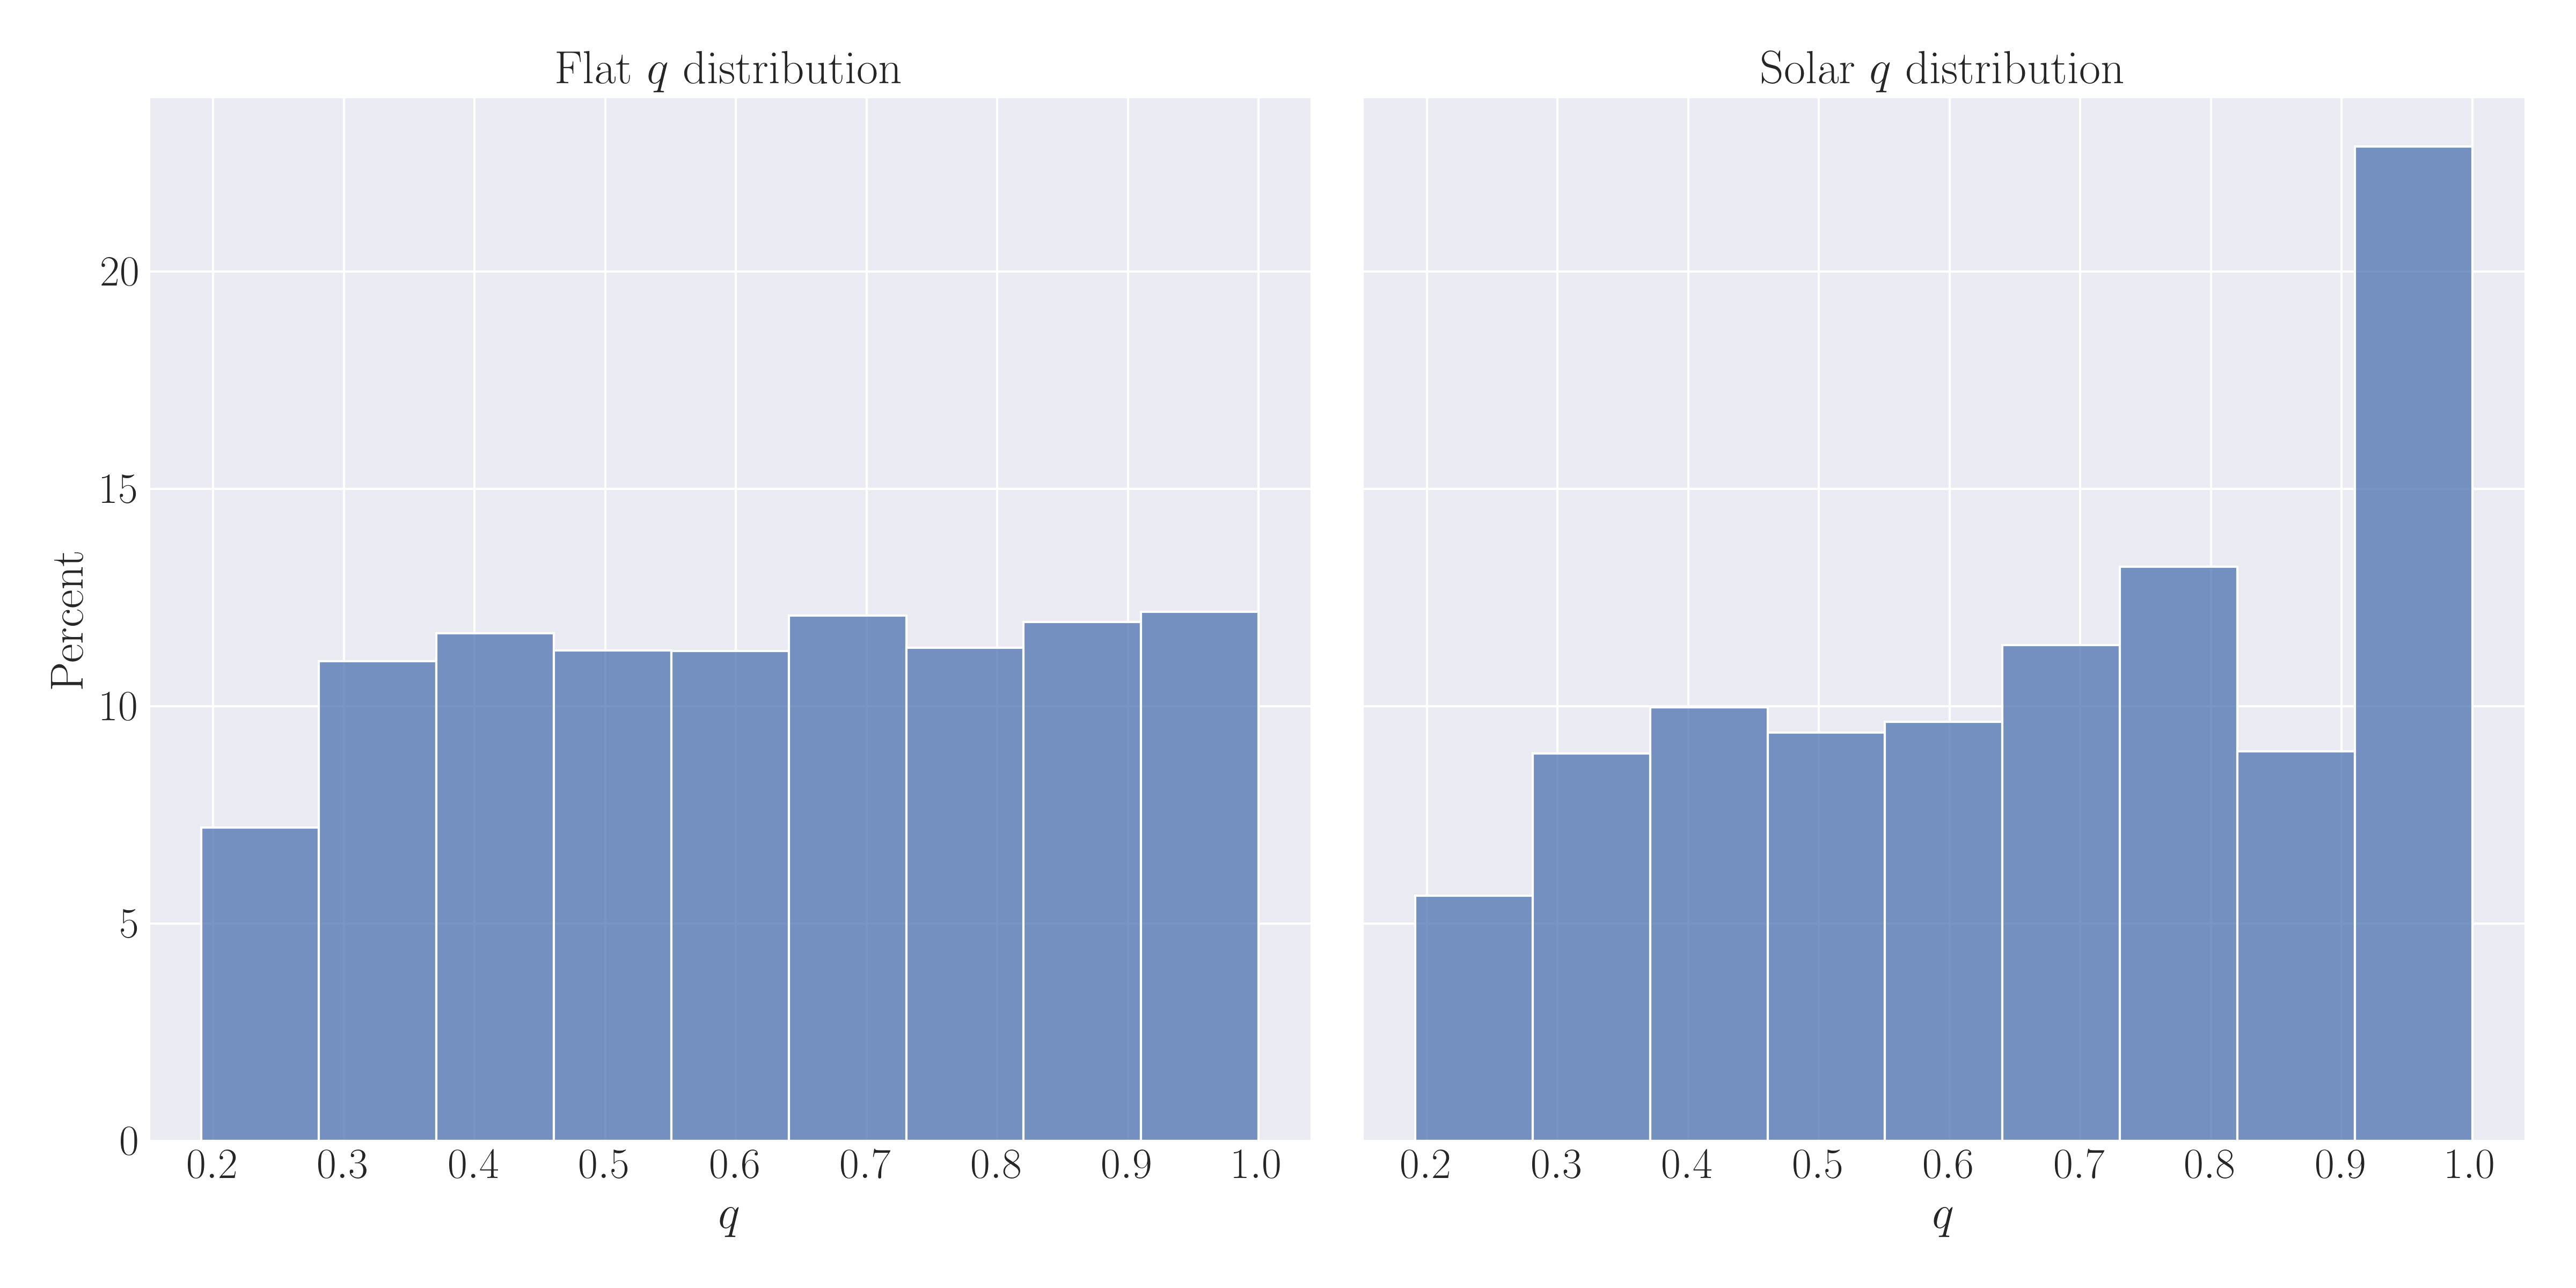
\includegraphics[width=\textwidth]{figures/q-dists.png}
    \caption{The resulting mass ratio distributions for the "flat" and "solar" mass ratio
        prescriptions. Both distributions are truncated and lowered at $q=0.2$ due to the relative
        lack low very low mass stars within the mass functions, making the creation of binary
        systems with a very low mass ratio impossible.}
    \label{fig:2/q-dists}
\end{figure}


After we have calculated the individual binary fractions for each value of $q$, we then go through
each bin of main-sequence stars and attempt to make binaries. The companion mass for a given bin is
calculated using the current value of $q$ and the number of binaries to make is calculated using the
binary fraction for the current value of $q$. After the companion mass and number of binaries are
set, we then find the closest bin to the companion mass and subtract from the primary and companion
bins the mass corresponding to the calculated number of binaries, adding the subtracted mass to a
new bin with a mean mass equal to the sum of each binary component.


We repeat this process for each bin of main-sequence stars until all bins have a binary fraction
corresponding to the weighted $f_b$ of the current value of $q$. We do this process for each value
of $q$ in the mass ratio distribution, resulting in each main-sequence bin having a binary fraction
equal to the total requested binary fraction and a mass ratio distribution identical to the
requested distribution.


This process tends to create on the order of 150 new bins in our mass function which dramatically
increases the runtime of the \code{LIMEPY} models. In order to prevent this we group together binary
bins of similar masses, forming 15 binary bins containing binary systems of similar total mass but
differing mass ratios. Figure \ref{fig:2/shifted-mf} shows the original main sequence bins, plotted
with the modified main sequence bins, binary bins and rebinned binary bins.


\begin{figure}
    \centering
    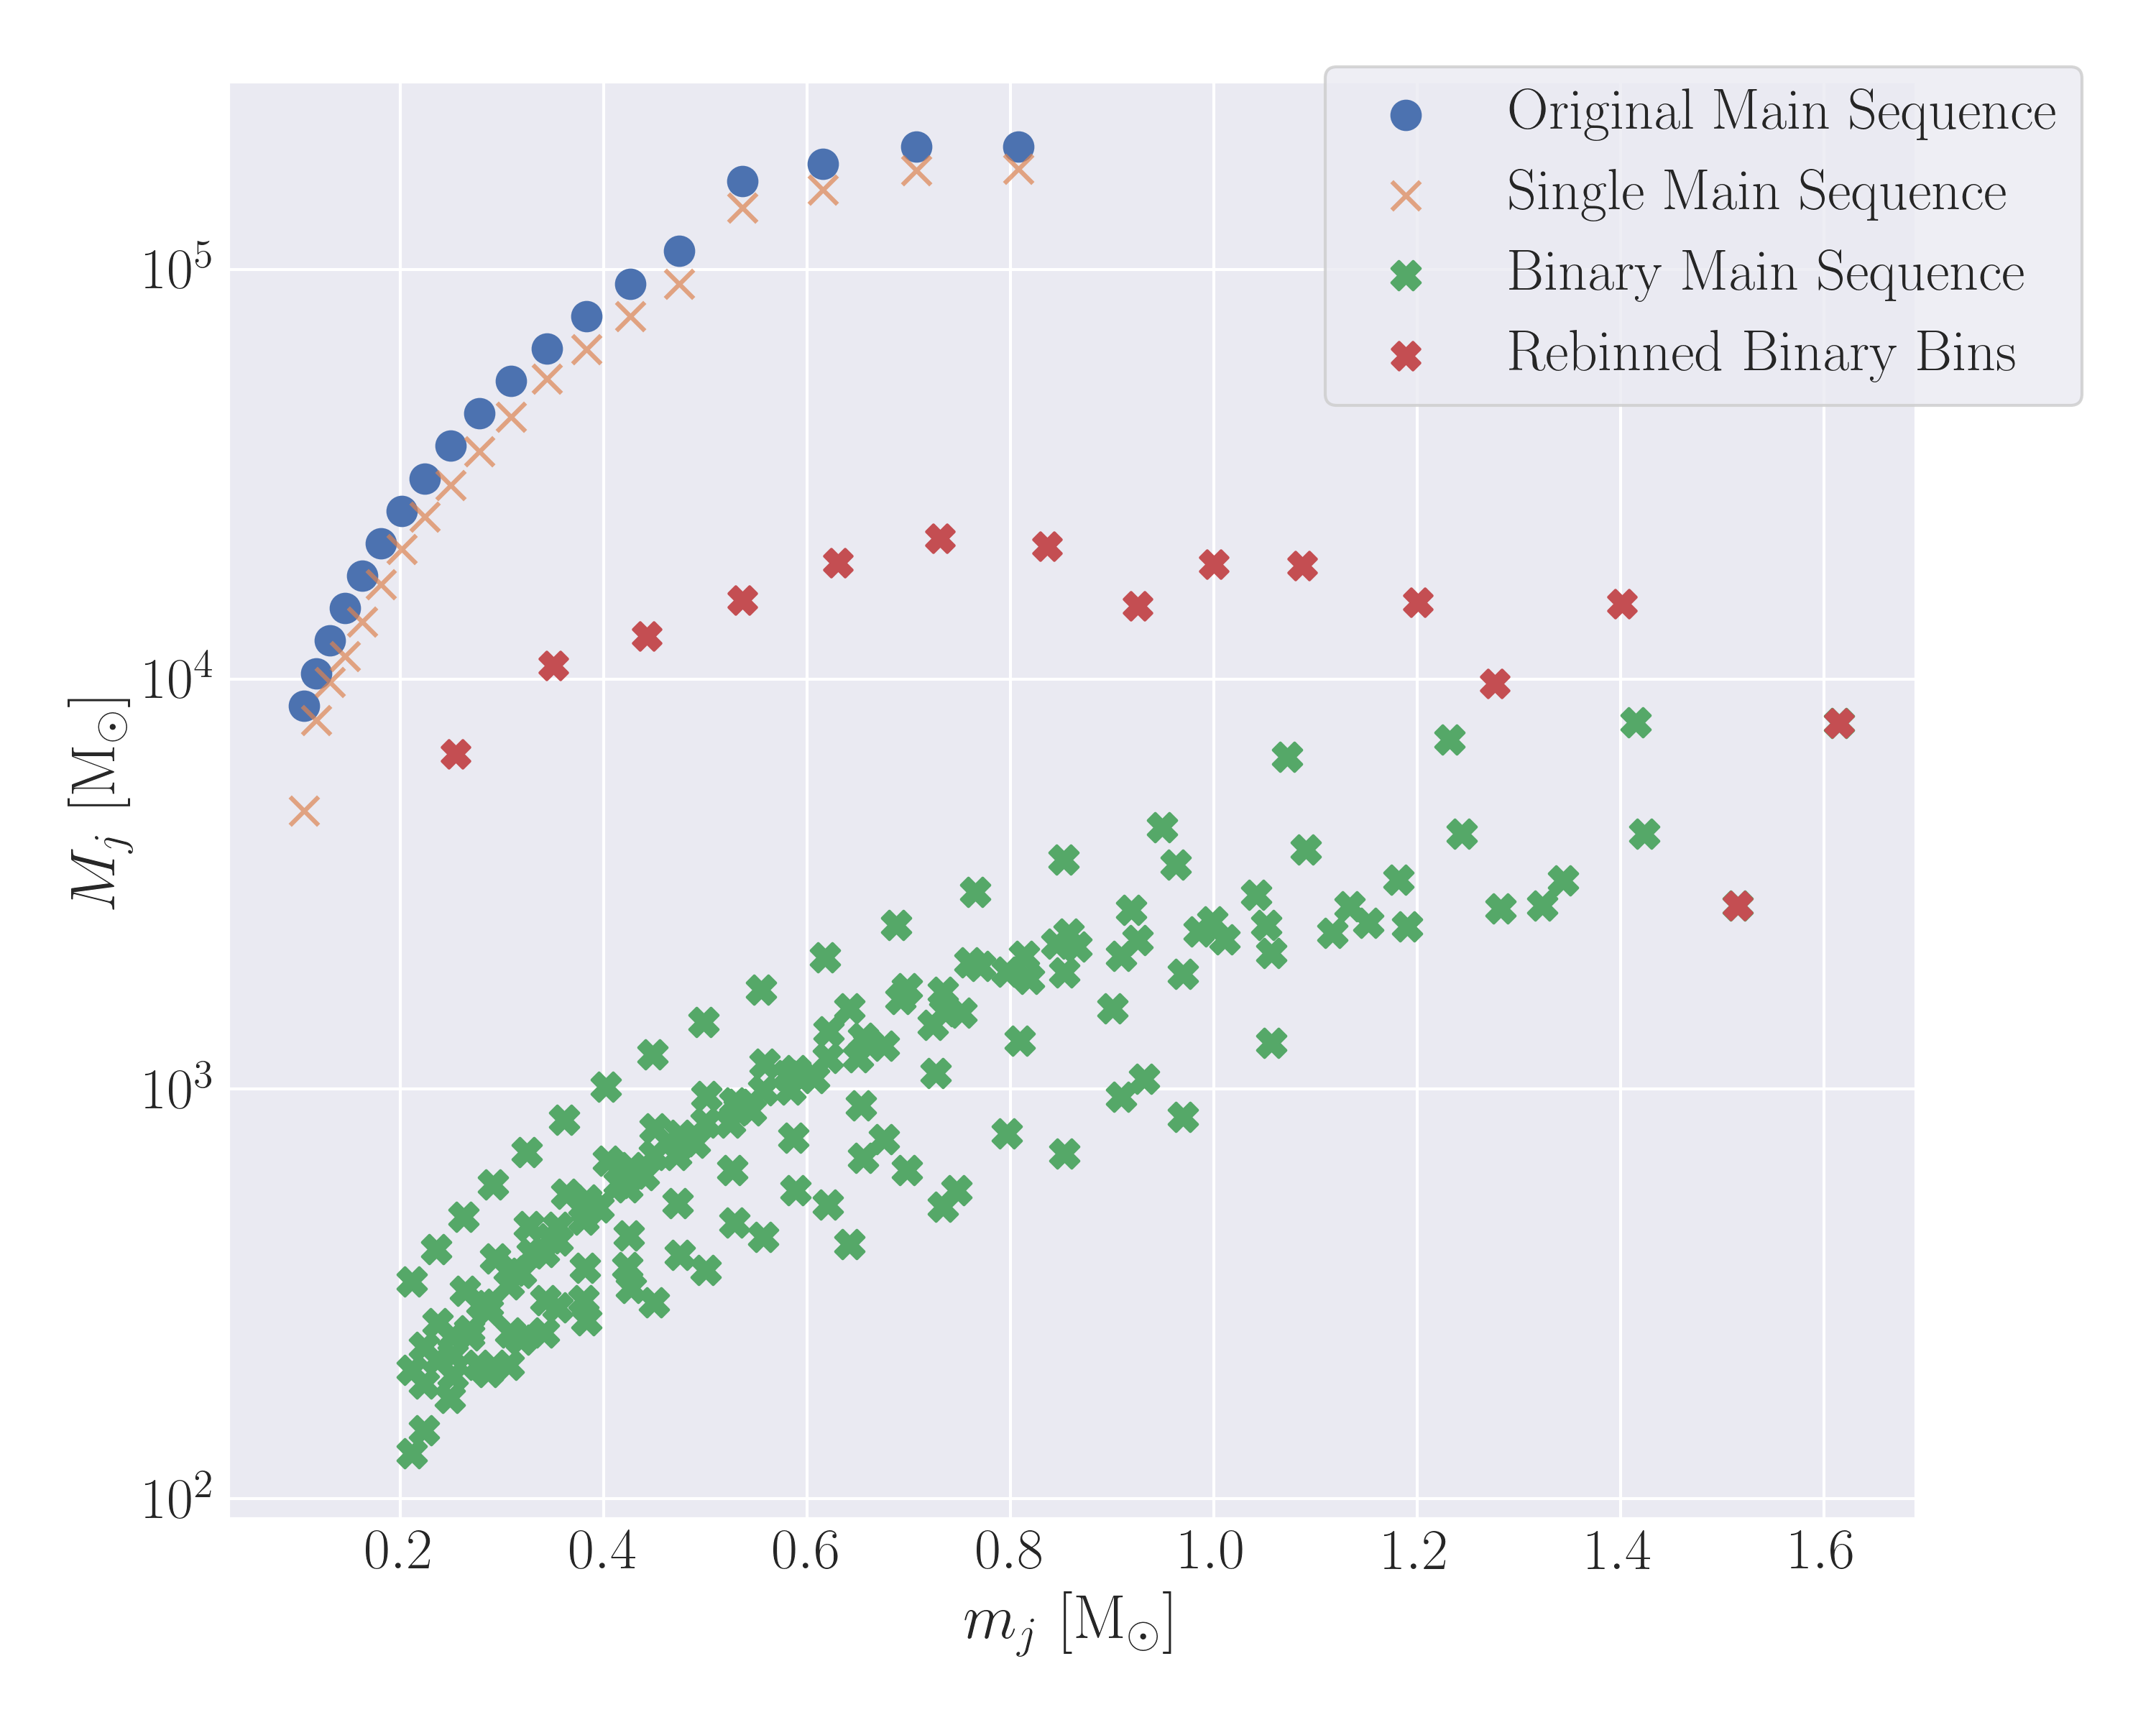
\includegraphics[width=0.8\textwidth]{figures/shifted-mf.png}
    \caption{The main-sequence portion of a mass function before and after binaries are added. The
        blue circles are the original main sequence and the crosses are the modified main sequence.
        The orange crosses show the single stars after mass has been removed to create binaries and
        the many green crosses are the binary bins that are initially created. The red crosses are
        the rebinned binary bins which are actually used in the computation of the \code{LIMEPY}
        models.}
    \label{fig:2/shifted-mf}
\end{figure}



\section{Fitting Models to Data}


To fit our models to the data we use the \code{GCfit}
package\footnote{\url{www.github.com/nmdickson/gcfit}}. \code{GCfit} provides a uniform interface
for fitting \evolvemf{} and \code{LIMEPY} models to observations of clusters using either MCMC or
Nested Sampling.

For this project we use the MCMC backend which is powered by \code{EMCEE}
\citet{Foreman-Mackey2013,Foreman-Mackey2019}. We use 1024 walkers, initialized at a reasonable
estimate of the best-fit parameters. We run the chain for at least 2000 steps and discard the
initial burn-in period.

\subsection{Likelihoods}

The majority of the likelihood functions we use are simple Gaussian likelihoods of the following
form:

\begin{equation}
    \ln \left(\mathcal{L}\right)=\frac{1}{2}
    \sum_{r}\left(\frac{\left(\sigma_{\mathrm{obs}}(r)
        -\sigma_{\mathrm{model}}(r)\right)^{2}}{\delta \sigma_{\mathrm{obs}}^{2}(r)}
    -\ln \left(\delta \sigma_{\mathrm{obs}}^{2}(r)\right)\right)
\end{equation}

Where $\mathcal{L}$ is the likelihood, $\sigma$ is the line-of-sight velocity dispersion, $r$ is the
projected distance from the cluster centre, and $\delta \sigma$ is the uncertainty in the velocity
dispersion. The likelihoods for other observables are formulated in the same way, and the specifics
are discussed in \code{GCfit}'s documentation\footnote{\url{gcfit.readthedocs.io}}. The total
likelihood is therefore the sum of all the log-likelihoods for each set of observations.

For the mass function and number density likelihoods we include additional nuisance and scaling
terms to account for extra sources of error in the mass function data and the effects of potential
escapers at the cluster boundary.

\subsubsection{Pulsar Likelihood}

\ps{I think we might want more detail here}

As stated previously, the development of a method to use pulsar acceleration measurements to
constrain the models was performed as part of an earlier project, but we will provide a brief
description of the likelihood function.

In order to assign a likelihood to a particular acceleration measurement we first use the
\texttt{LIMEPY} models to generate a line-of-sight acceleration profile for the given model. We then
use this acceleration profile to interpolate the possible line-of-sight positions for the pulsar.
These line-of-sight positions are then assigned a likelihood based on a Gaussian centred at the
line-of-sight position as calculated from either the dispersion measure (DM) of the pulsar or the
density of pulsar-mass objects at that radius. This likelihood distribution is then convolved with a
Gaussian distribution representing the error on the pulsar's acceleration measurement. A resulting
probability distribution from this method is shown in Figure \ref{fig:pulsar-likelihood}.

\begin{figure}
    \centering
    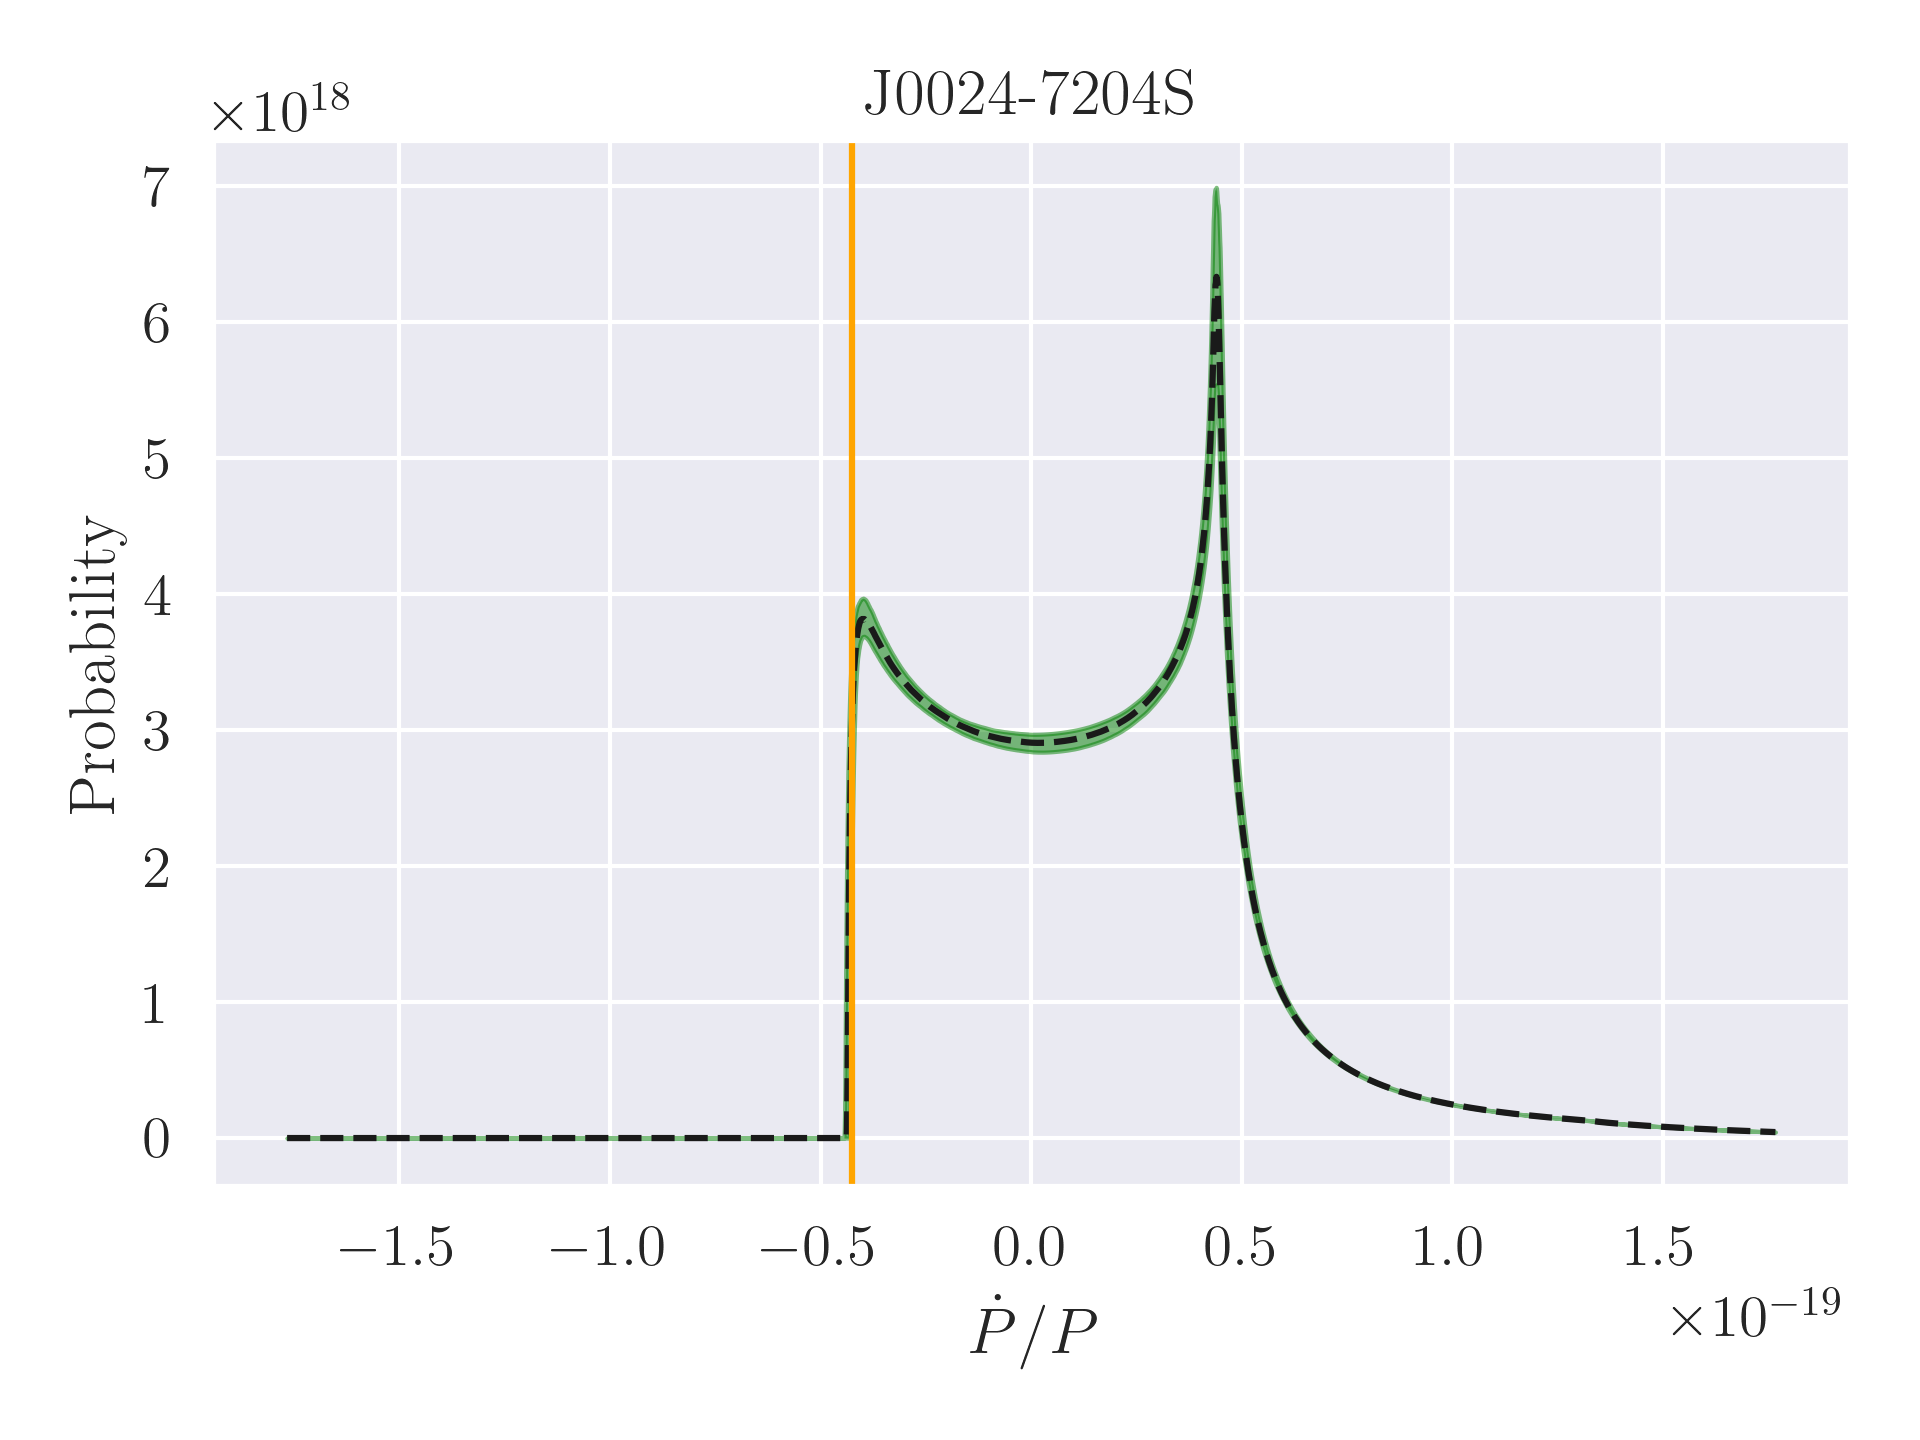
\includegraphics[width=0.8\textwidth]{figures/pulsar-likelihood.png}
    \caption{The resulting probability distribution for period derivatives of pulsar 47\,Tuc S from
        the method described above. The green line is the likelihood of a given period
        derivative measurement and the yellow line is the measured period derivative. The asymmetry in
        the distribution is due to the intrinsic spin-down of the pulsar, biasing the distribution to
        positive values of $\dot{P}/P$.}
    \label{fig:pulsar-likelihood}
\end{figure}




\subsection{Fitting Mass Functions to Observations}

When the mass function data was originally collected, the mass was recorded based on the position of
the star on an isochrone fit to the cluster (see \citealt{Sollima2017} for details). This means that
any binary stars in the sample are recorded as single stars a mass corresponding to a star with the
combined colour of the two binary components and a luminosity corresponding to the sum of the two
components.

Additionally, when we move mass around to create binary bins we remove mass from the surface density
profiles which would normally be compared to the mass function data. In order to compensate for
these effects, we rescale the surface density profiles to include the stars which are in binary
bins, according to how they would have been observed using the observational method described above.

In order to determine the observed mass we use a grid of MIST isochrones
\citep{Dotter2016,Choi2016}\footnote{We use the \code{EZMIST} library to fetch and prepare the
isochrones. \code{EZMIST} is available online: \url{https://github.com/mfouesneau/ezmist}} computed
at a range of metallicities, at the age of the cluster. We use the isochrone closest to the model
parameters to determine the luminosity of the binary components and then again use the isochrone to
determine the observed mass of the combined luminosities. Figure \ref{fig:2/isochrone} shows the
derived relation between stellar mass and luminosity used for these conversions. After having
determined at what mass a binary system would have been "observed", we then scale the surface
density profiles of the main-sequence bin which most closely matches the observed mass of the binary
system by the total mass of the binary system which allows us to correct for both effects.


\begin{figure}
    \centering
    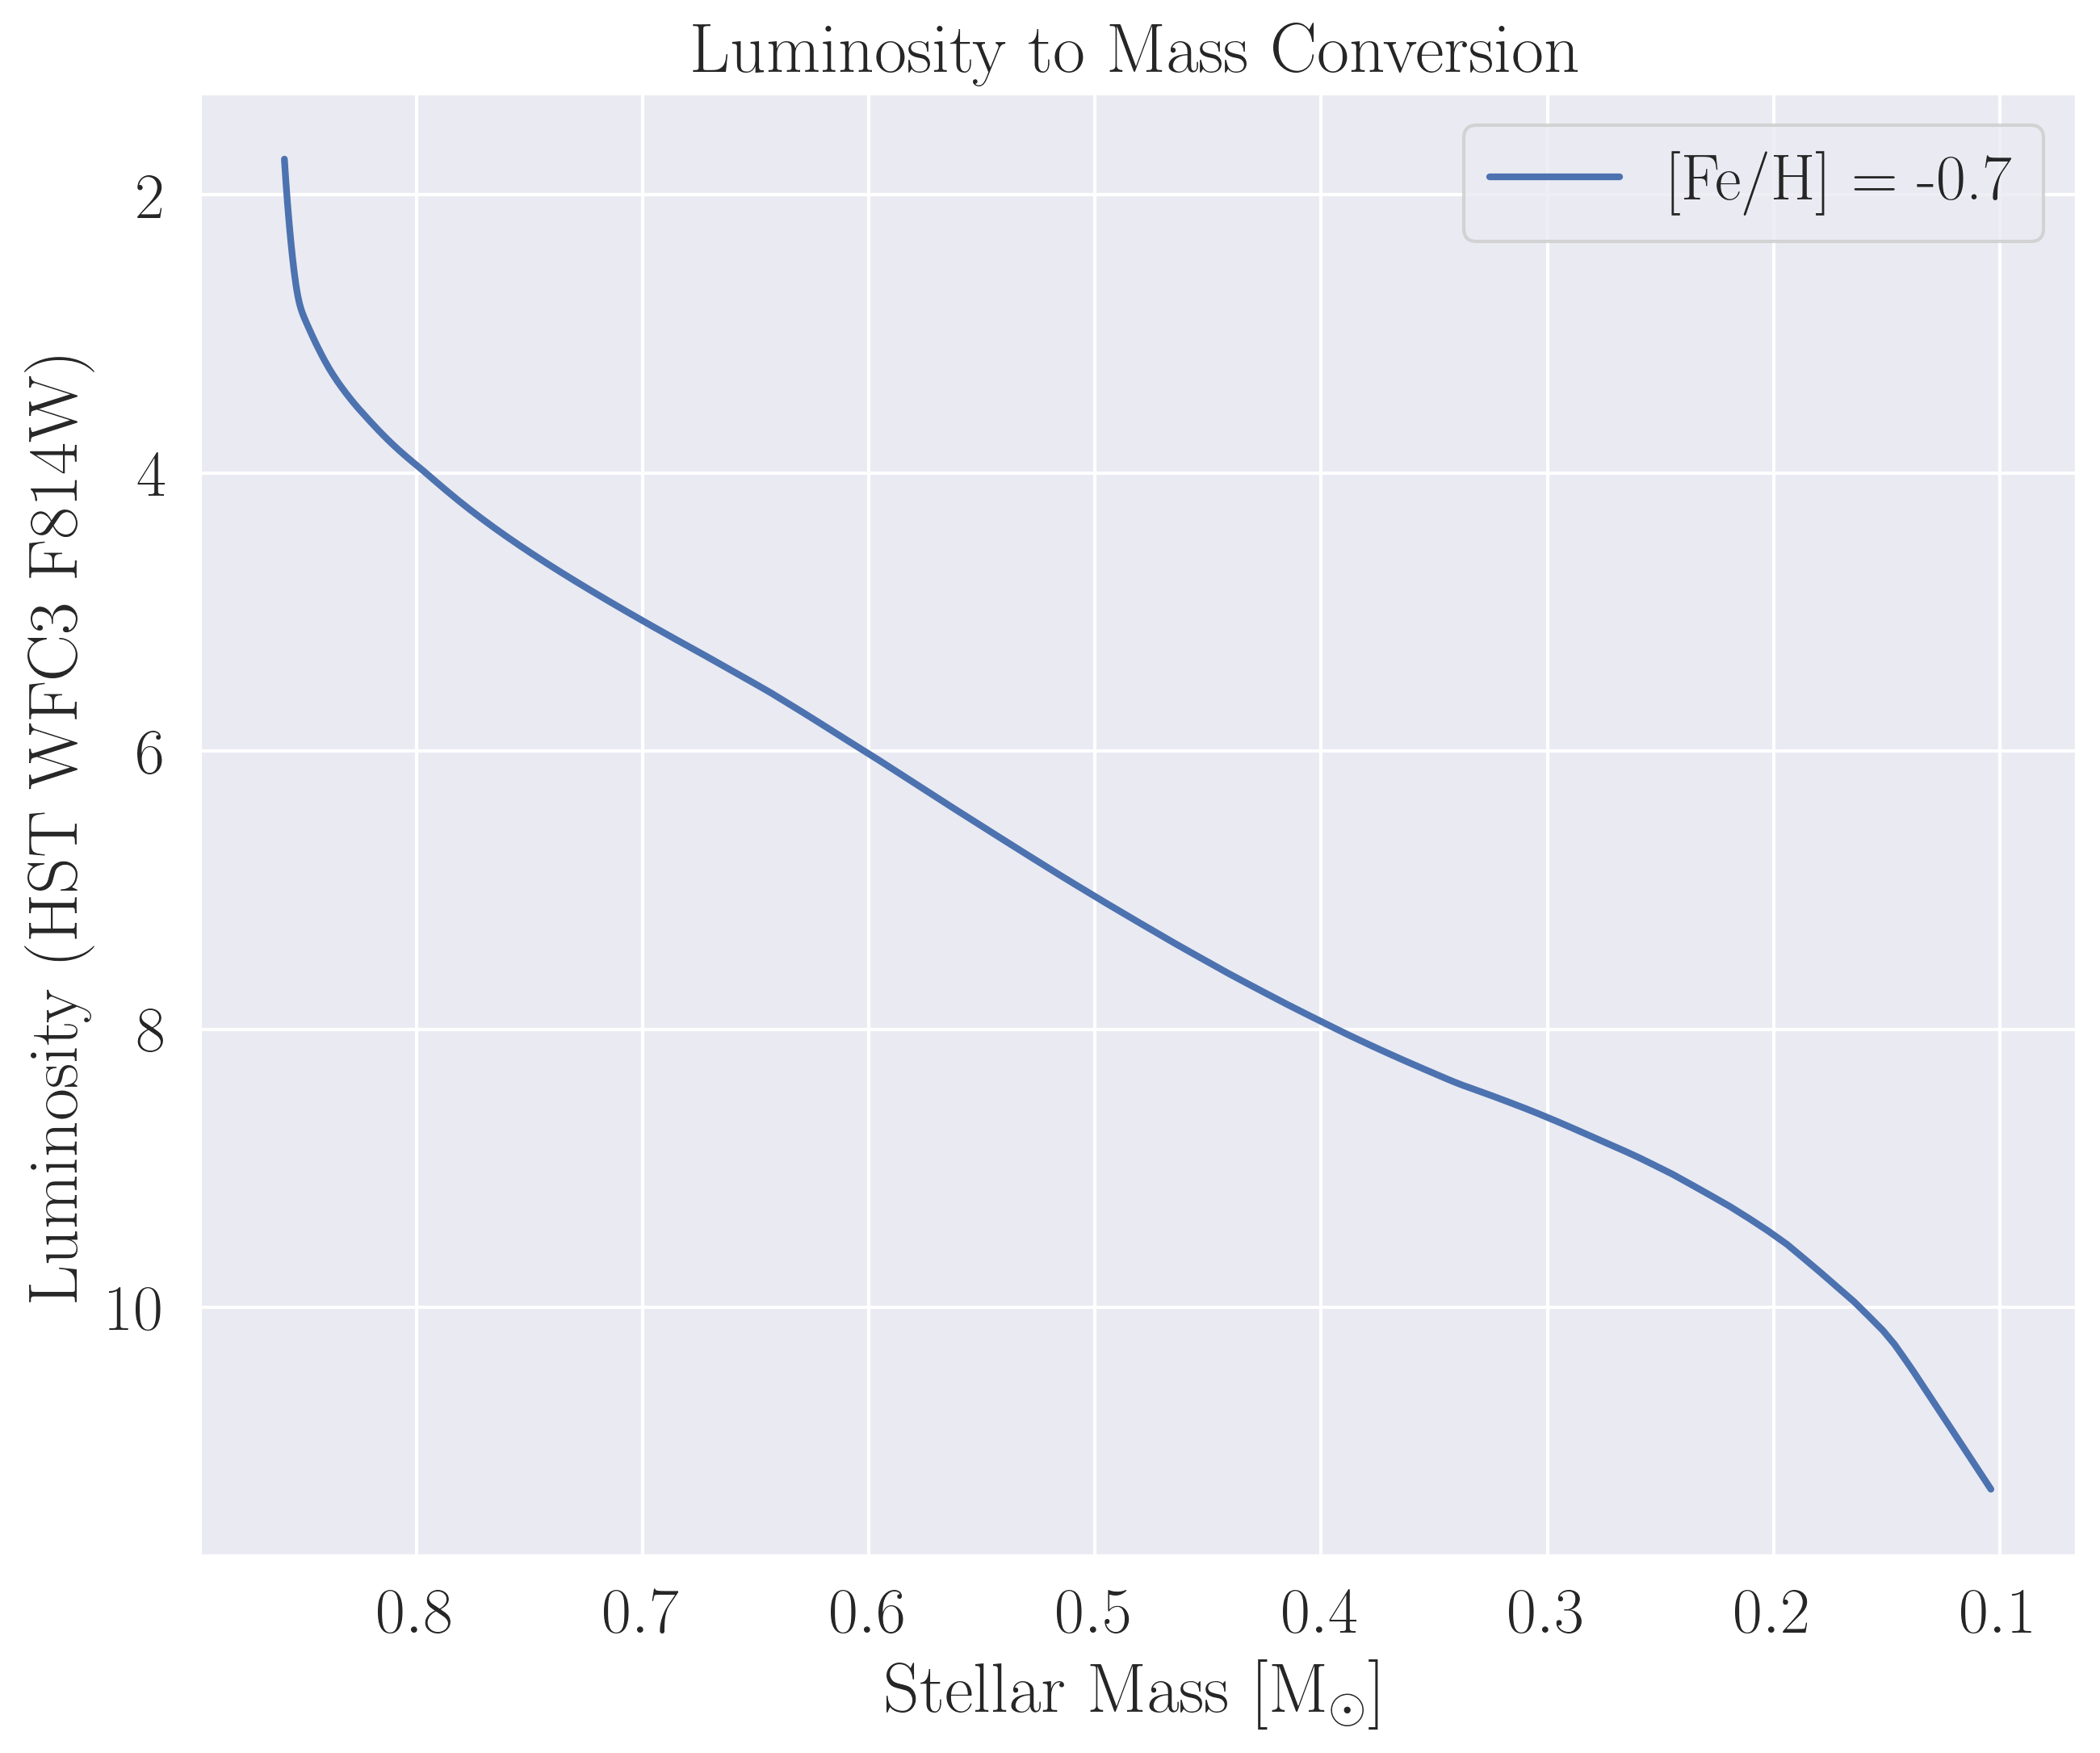
\includegraphics[width=0.8\textwidth]{figures/isochrone_conversion.png}
    \caption{Relation between stellar mass and luminosity through \emph{HST}/WFC3's F814W filter,
        derived from a MIST isochrone.}
    \label{fig:2/isochrone}
\end{figure}
\newpage


\chapter{Results}



\section{Results}



\subsection{Previous Results}

As mentioned previously, this project is a continuation of a project done over the previous year in
which we developed a method to use pulsar timing data to constrain our models. The final results of
that project were a set of models that accurately reproduce all observables and fully incorporated
the pulsar data. The best fit parameters of this set of models are listed in Table
\ref{tab:parameters_nobin}. Figure \ref{fig:nobin_obs_panel} shows the model fits to most of
the observables while Figure \ref{fig:nobin_mass_fun} shows the fit to the stellar mass function
data.

One of the most interesting results of the previous project was the models' ability to constrain the
black hole content within 47\,Tuc. Figure \ref{fig:prev_nobin_BH_dists} shows the distribution of
black hole mass and number in  our set of best fit models. Both the total mass and number are quite
well contained especially in comparison to the previous constraints in the literature \citep[see
	e.g.][]{Henault-Brunet2020,Weatherford2019}.


BH Mass [Msol] = 239.638 (+245.195 -145.800)
BH mass percentiles:
95: 679.2848600704087
99: 843.6530442277326
BH Number percentiles:
95: 89.77947118953271
99: 107.85053470005765
BH Number  = 41.143 (+27.184 -21.507)


% \begin{table}
% 	\centering
% 	\caption{Best fit parameters with $1-\sigma$ intervals.}
% 	\begin{tabular}{l l}

% 		\hline
% 		Parameter                 & Value                     \\
% 		\hline
% 		$\Phi_0$                  & $6.444^{+0.137}_{-0.126}$ \\
% 		$M/10^6 \mathrm{M}_\odot$ & $0.864^{+0.009}_{-0.009}$ \\
% 		$r_h / pc$                & $6.612^{+0.069}_{-0.067}$ \\
% 		$\log{r_a / pc}$          & $1.425^{+0.039}_{-0.035}$ \\
% 		$g$                       & $1.264^{+0.064}_{-0.072}$ \\
% 		$\delta$                  & $0.397^{+0.019}_{-0.020}$ \\
% 		$s^2$                     & $0.019^{+0.059}_{-0.013}$ \\
% 		$F$                       & $2.972^{+0.019}_{-0.039}$ \\
% 		$\alpha_1$                & $0.468^{+0.047}_{-0.041}$ \\
% 		$\alpha_2$                & $1.178^{+0.053}_{-0.057}$ \\
% 		$\alpha_3$                & $2.117^{+0.039}_{-0.038}$ \\
% 		$BH_{ret} (\%)$           & $0.128^{+0.084}_{-0.061}$ \\
% 		$d$                       & $4.433^{+0.021}_{-0.023}$ \\
% 		\hline
% 	\end{tabular}
% 	\label{tab:parameters_nobin}
% \end{table}

% \begin{figure}
% 	\centering
% 	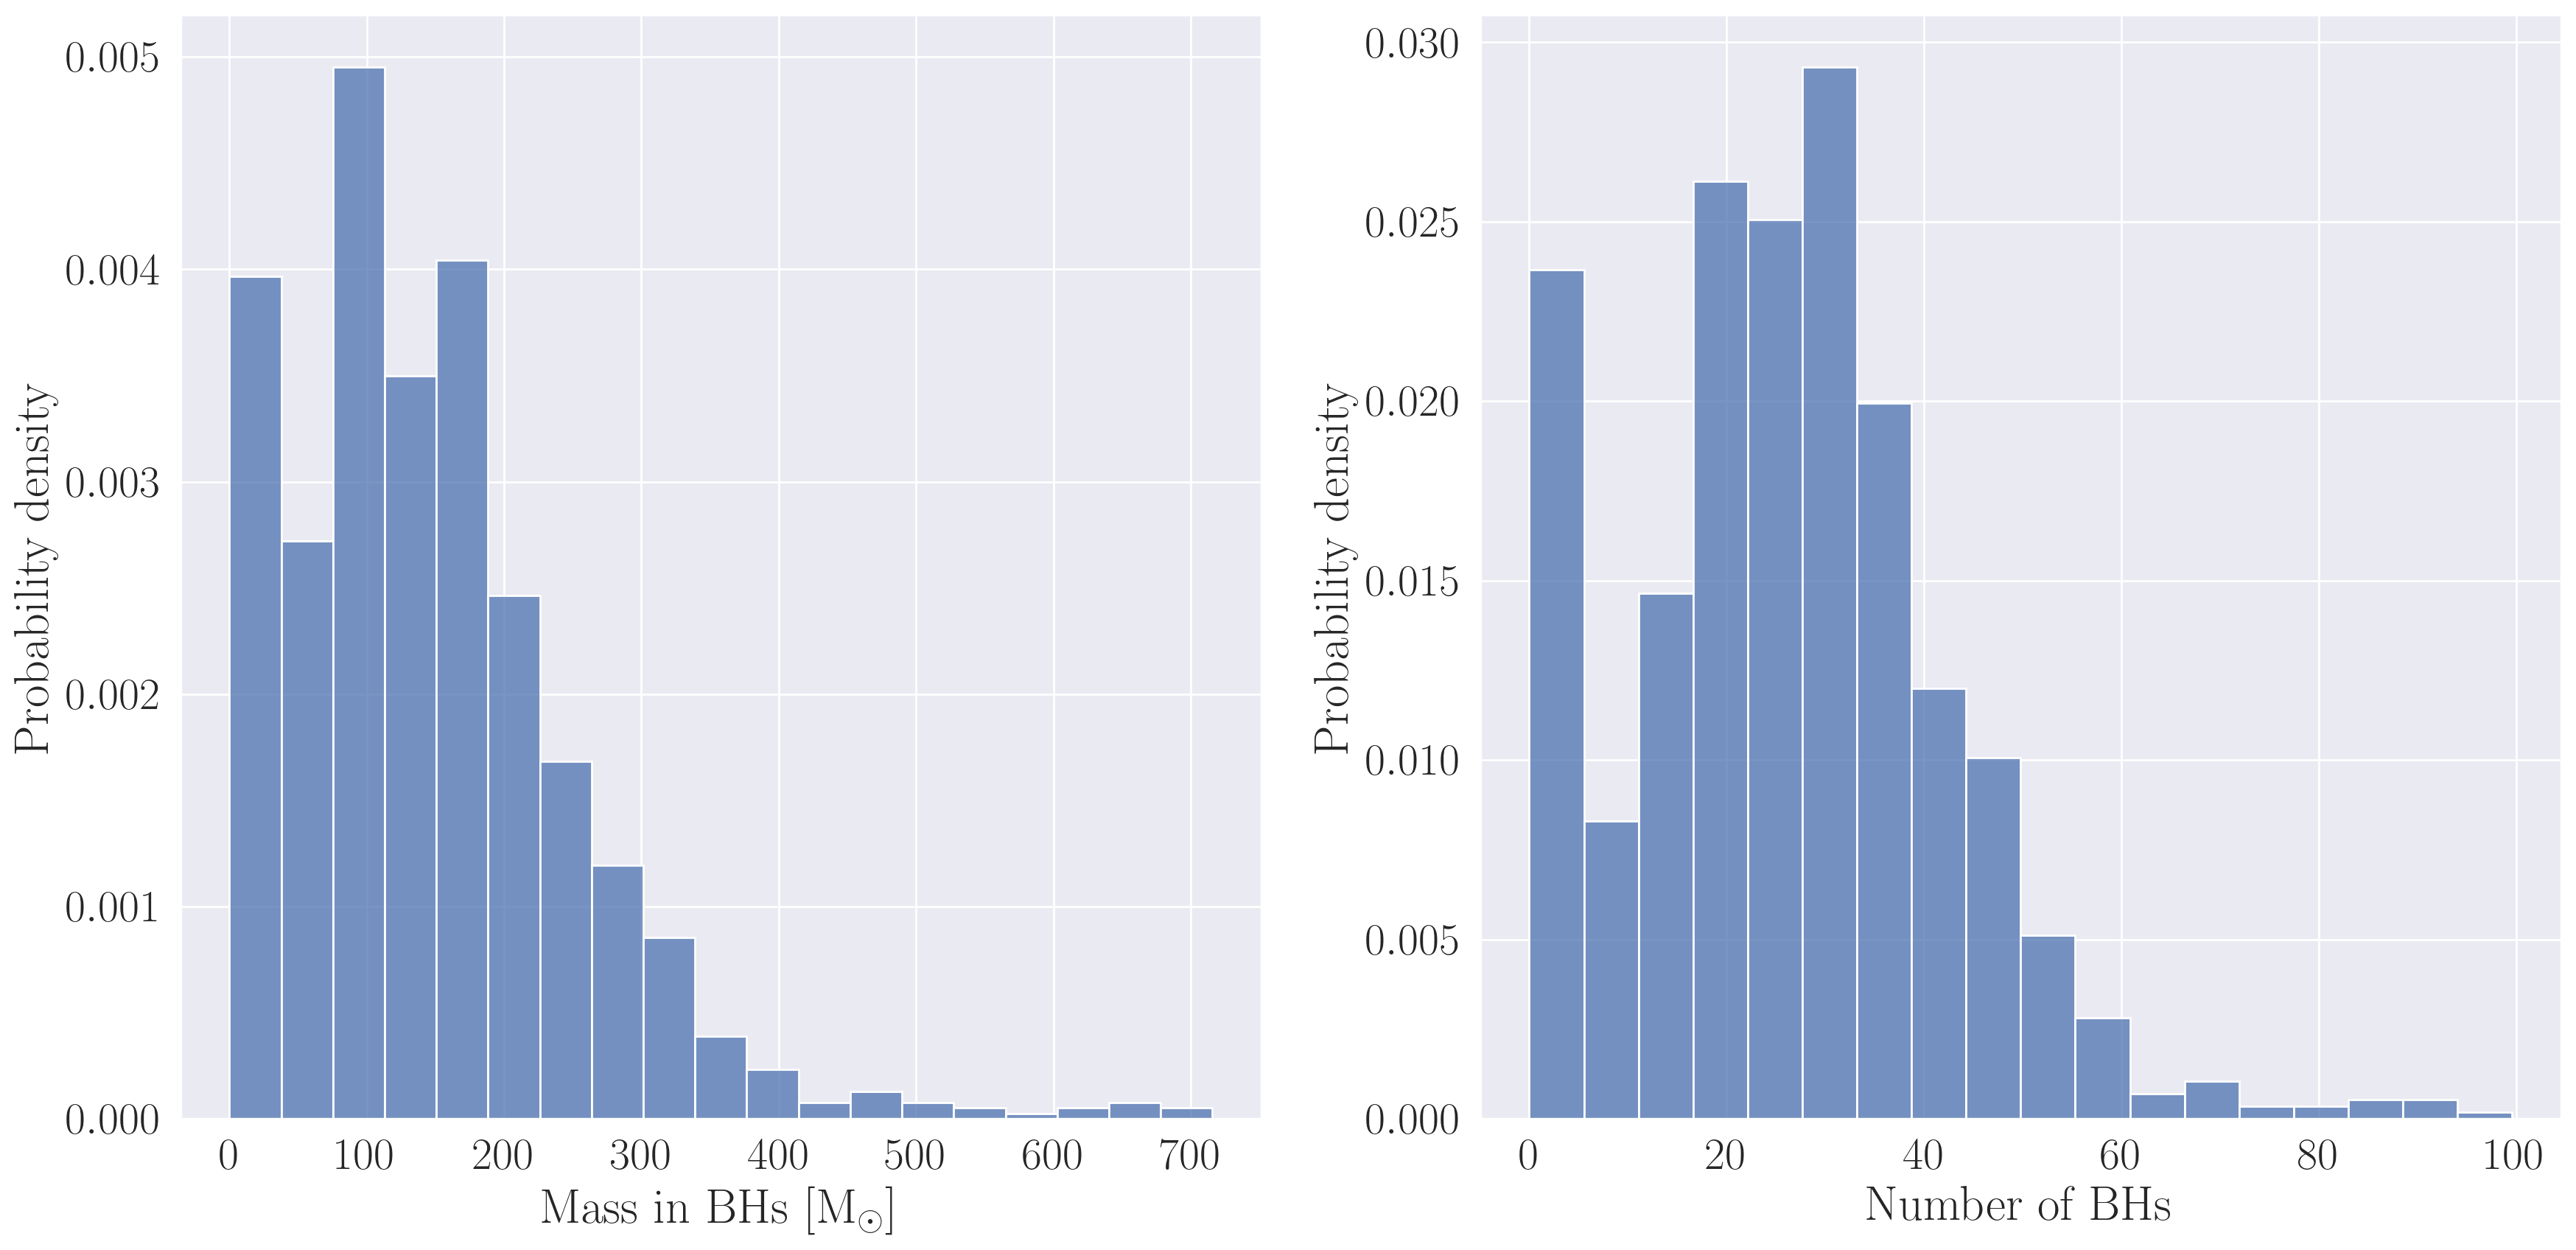
\includegraphics[width=0.8\textwidth]{figures/prev_nobin/BH_dists.png}
% 	\caption{BH distributions}
% 	\label{fig:prev_nobin_BH_dists}
% \end{figure}


\subsection{Low Binary Fraction}
\ps{Describe the results for the low binary fraction model.}


BH Mass: 114.252 solMass + 79.271 solMass - 144.032 solMass
BH Number: 22.058 + 13.407 - 18.533




In the low binary fraction case, the model is similar to the model without binaries. Maybe?

\ps{Figures with usual model quantities, also the binary mass histogram and the density profiles}


\begin{figure}
	\begin{center}
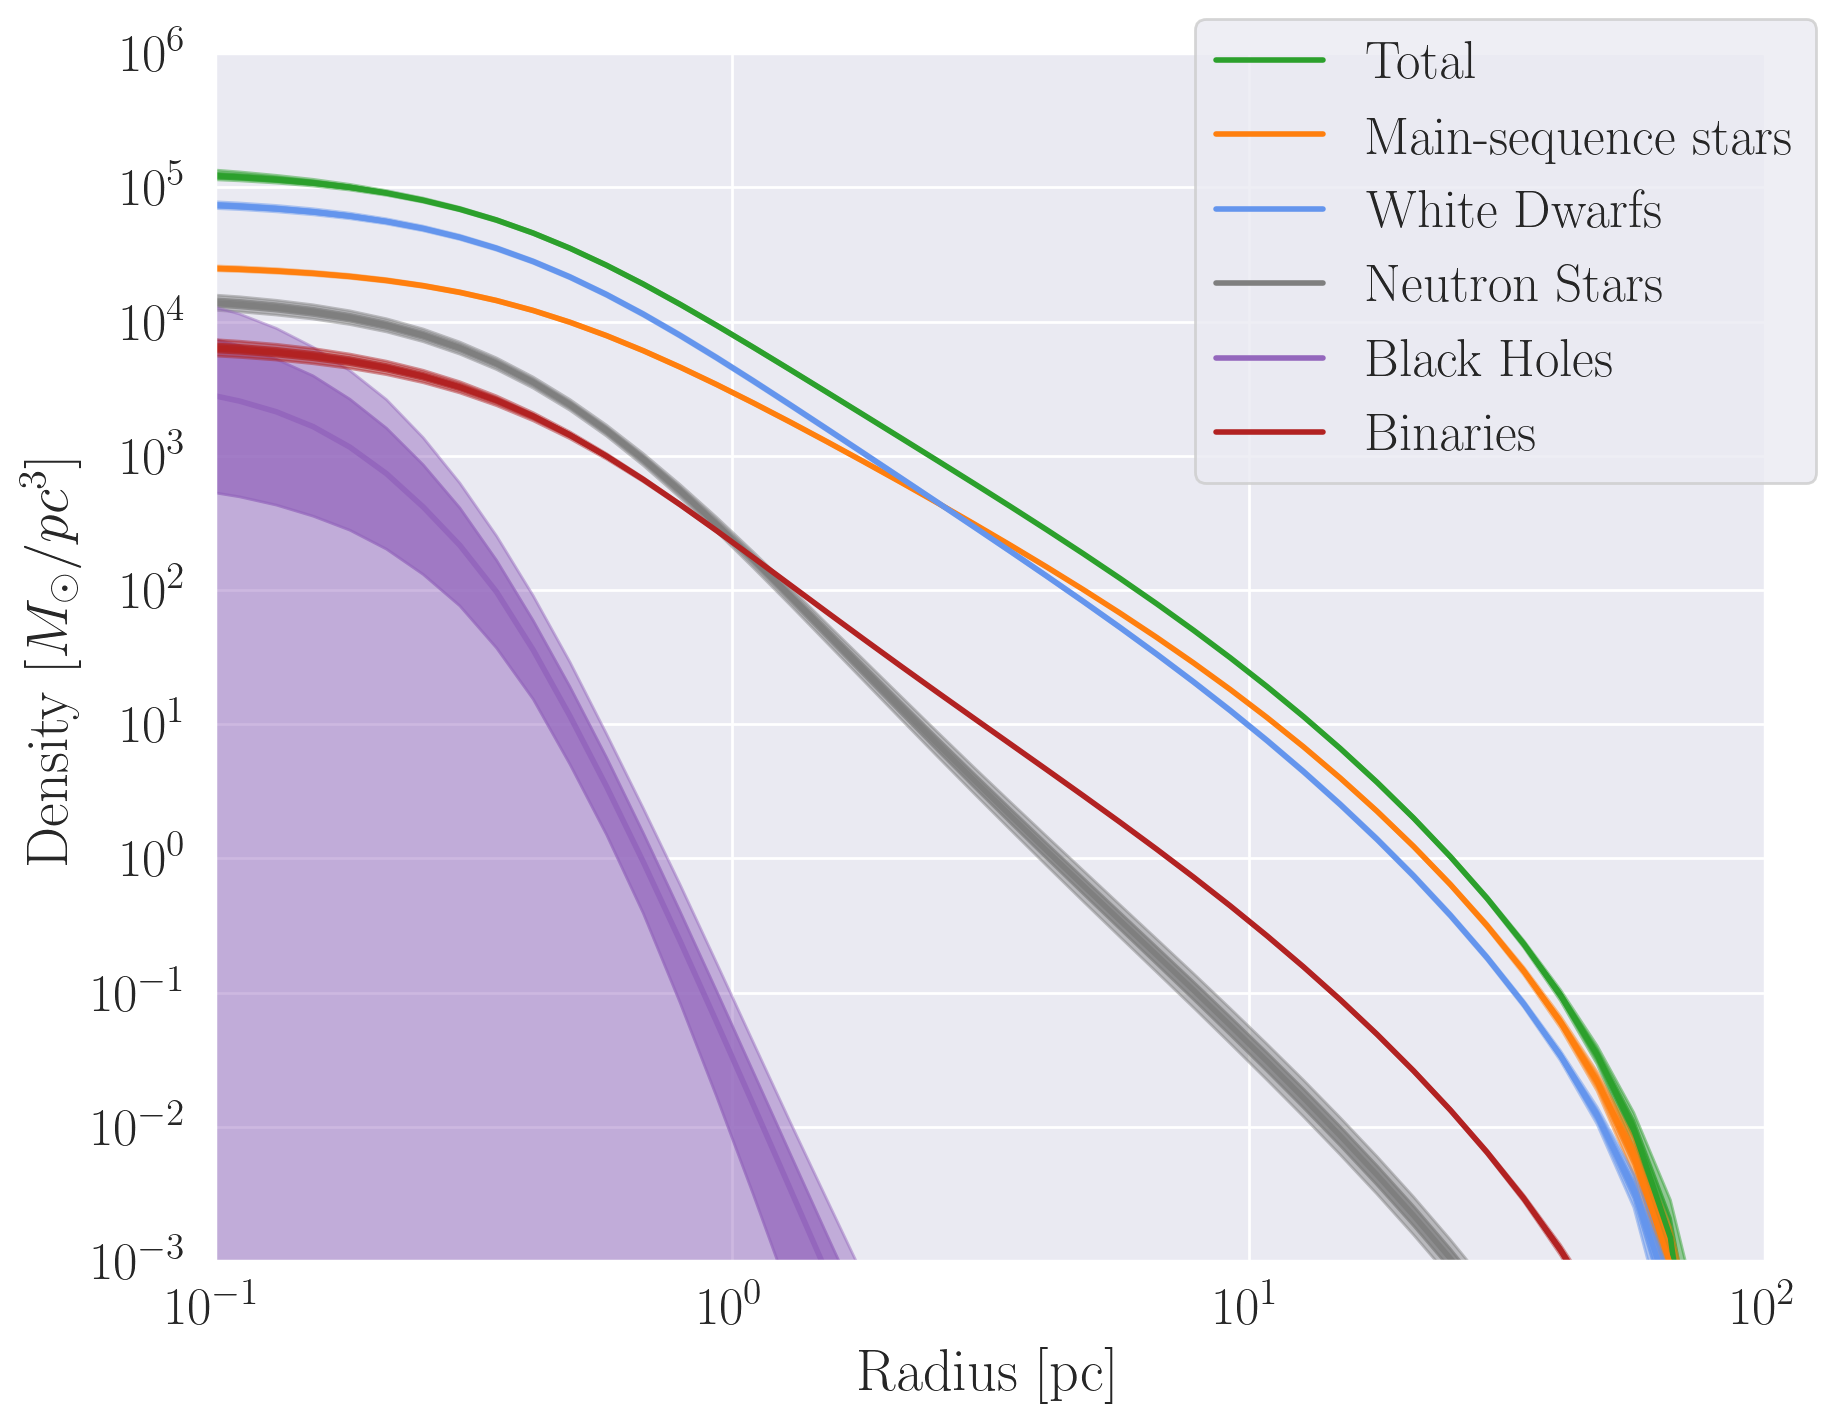
\includegraphics[width=0.9\textwidth]{figures/low_bin_model/density.png}
	\end{center}
\caption{Density Profiles}
	\label{fig:low_bin_model_densities}
\end{figure}

\begin{figure}
	\begin{center}
		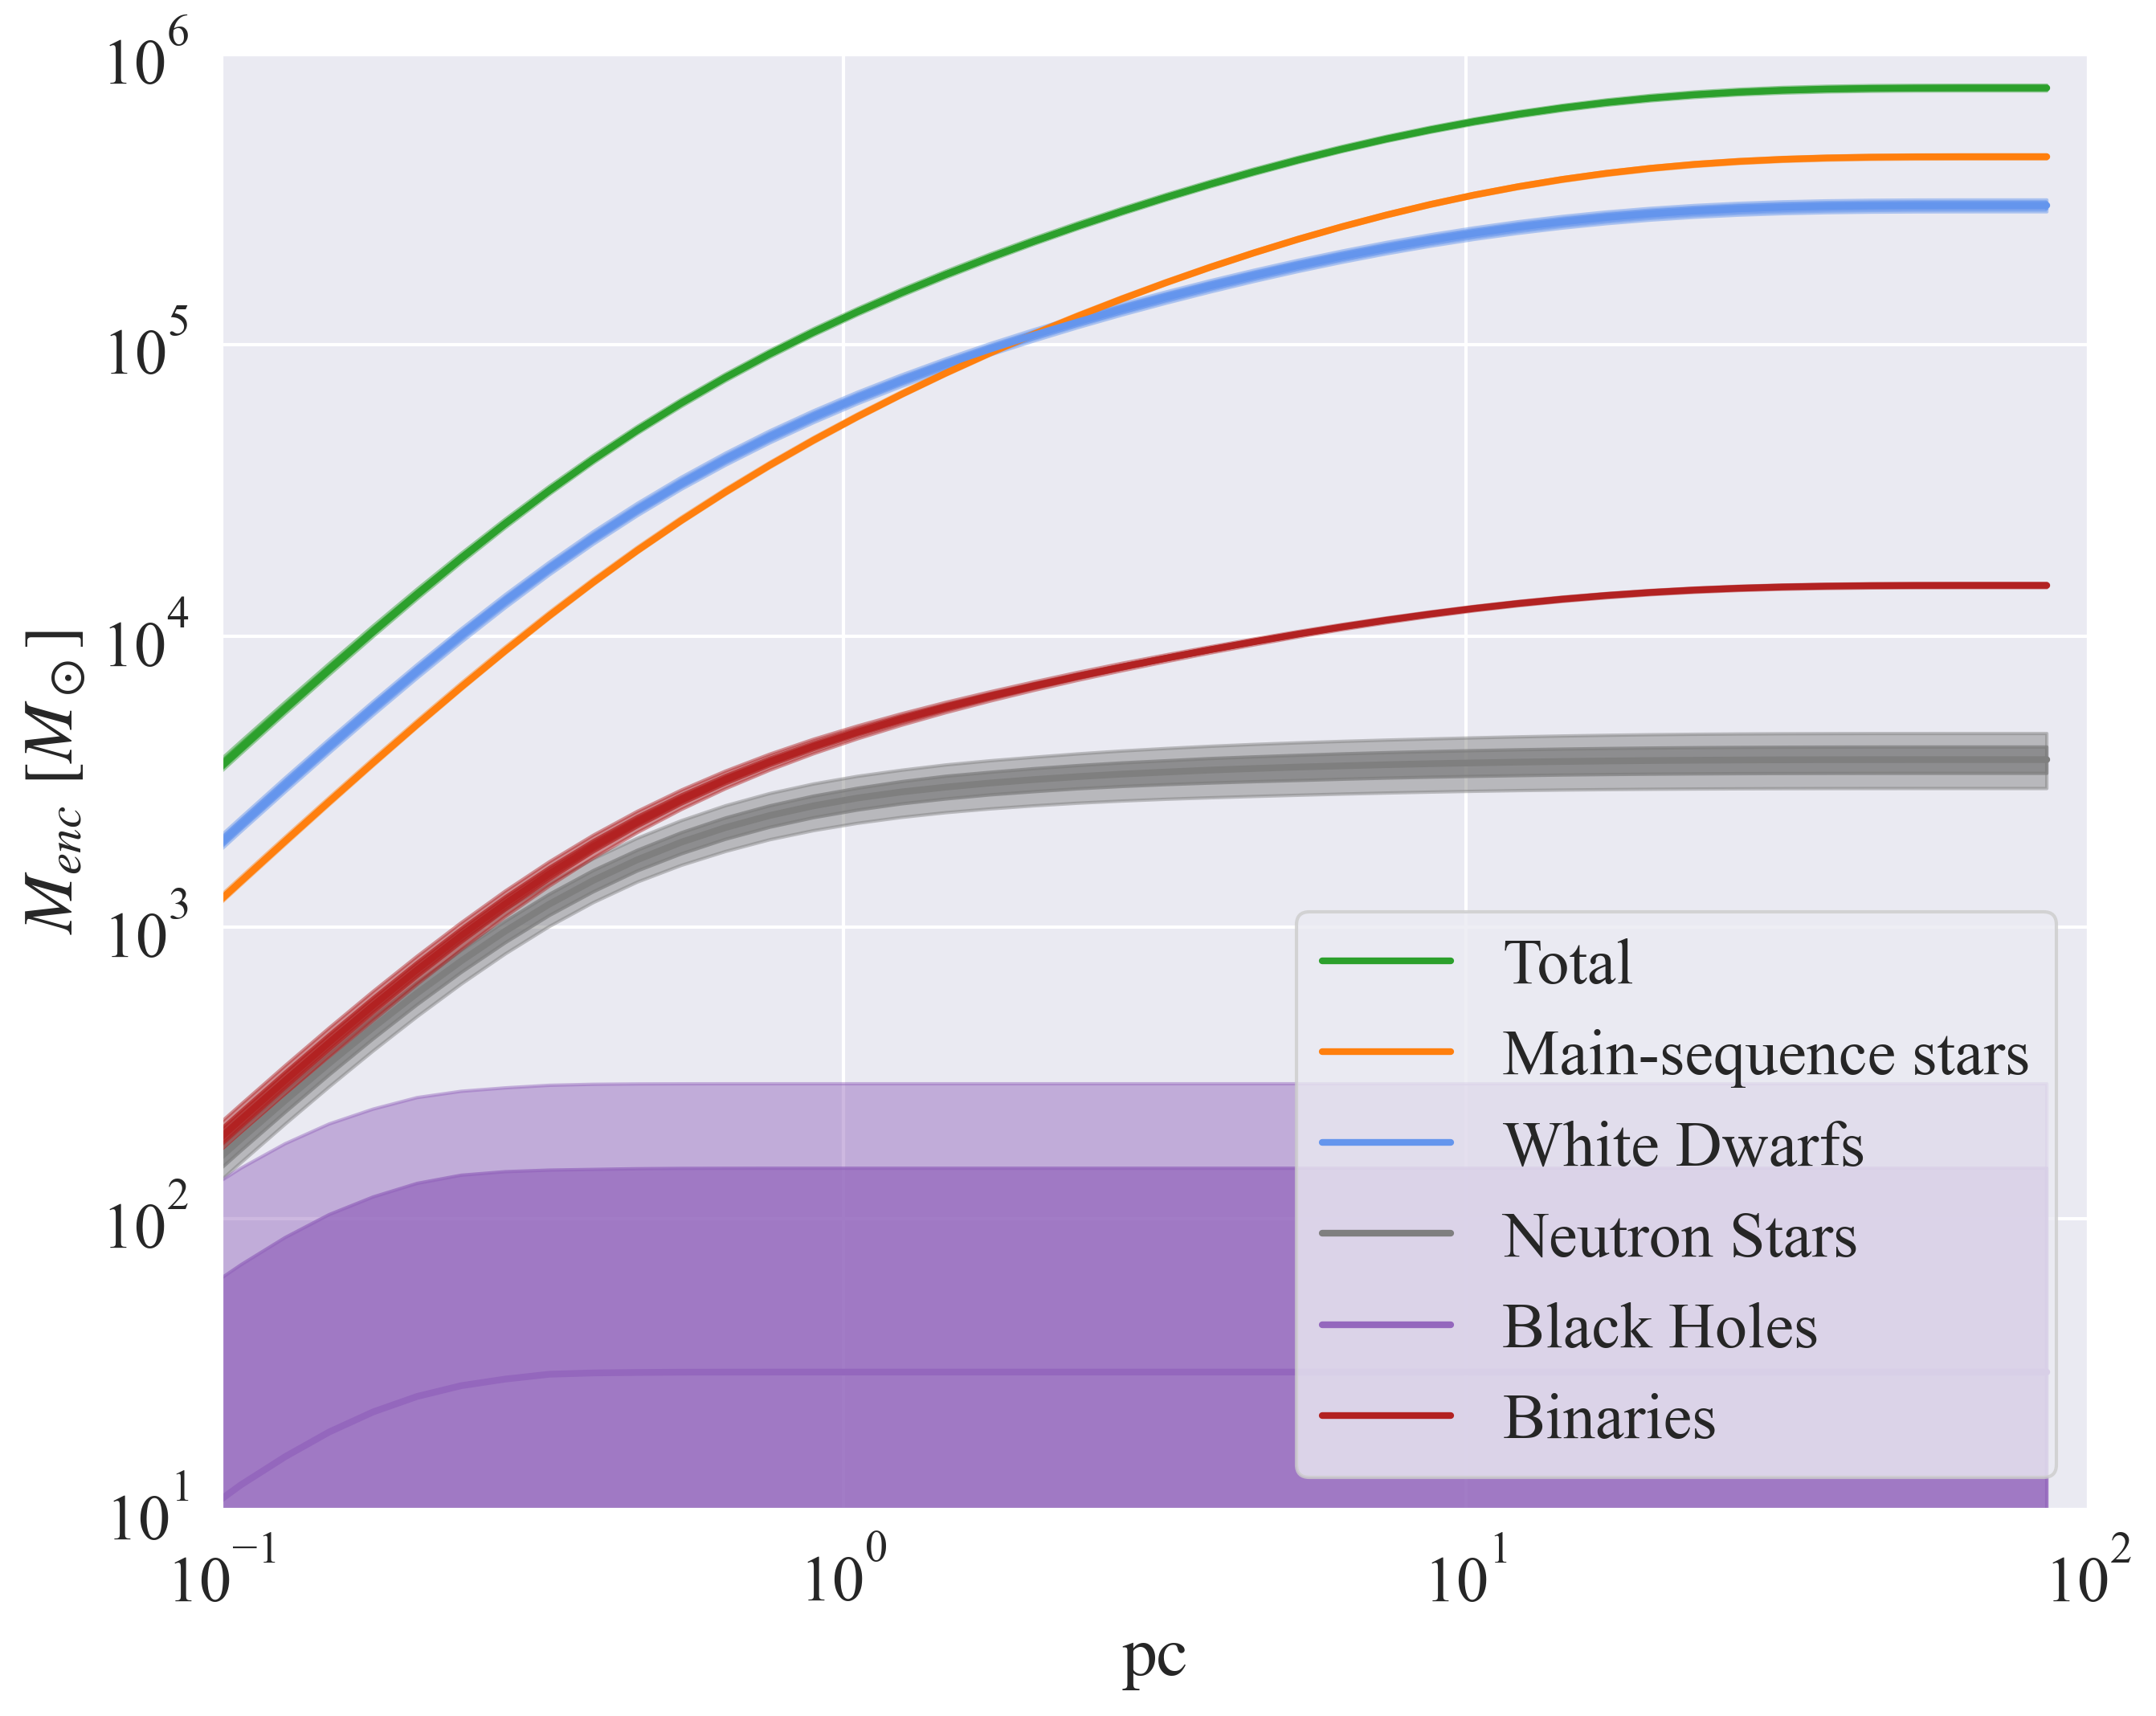
\includegraphics[width=0.9\textwidth]{figures/low_bin_model/mass_enc.png}
	\end{center}
	\caption{Density Profiles}
	\label{fig:low_bin_model_enclosed_mass}
\end{figure}

\begin{figure}
	\begin{center}
		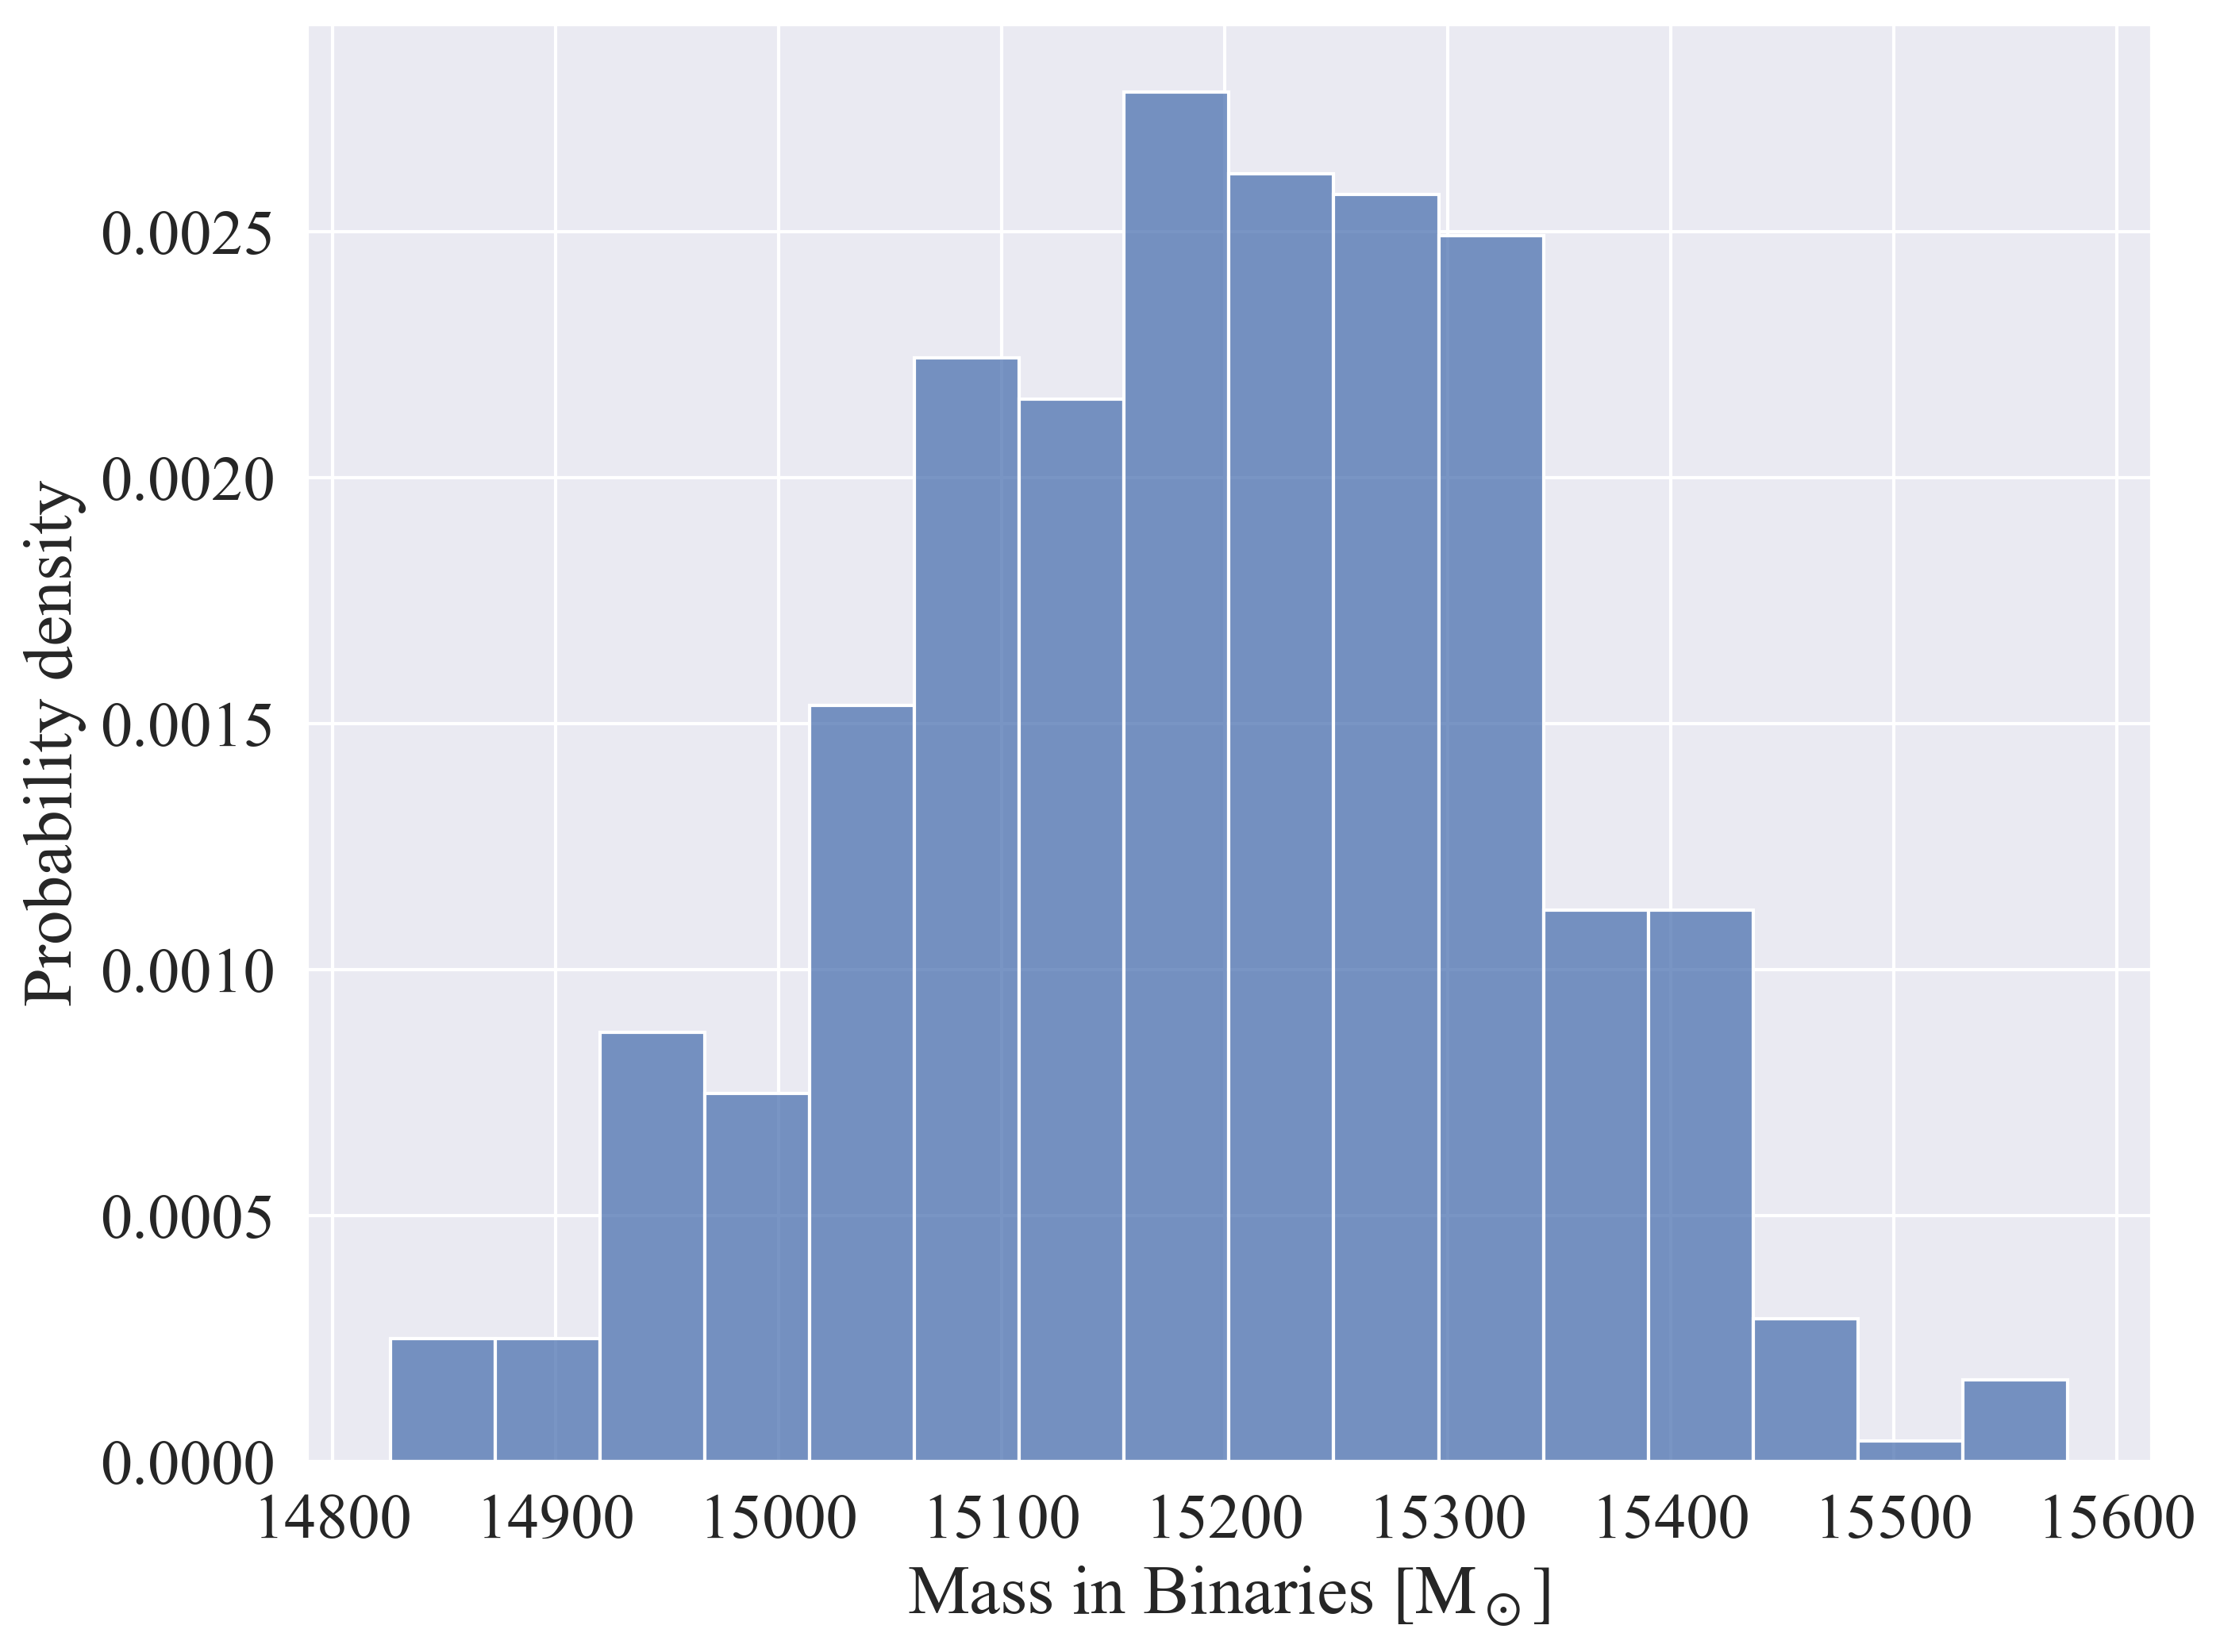
\includegraphics[width=0.9\textwidth]{figures/low_bin_model/binary_mass.png}
	\end{center}
	\caption{Total mass in binaries}
	\label{fig:low_bin_model_binary_mass}
\end{figure}

\begin{figure}
	\begin{center}
		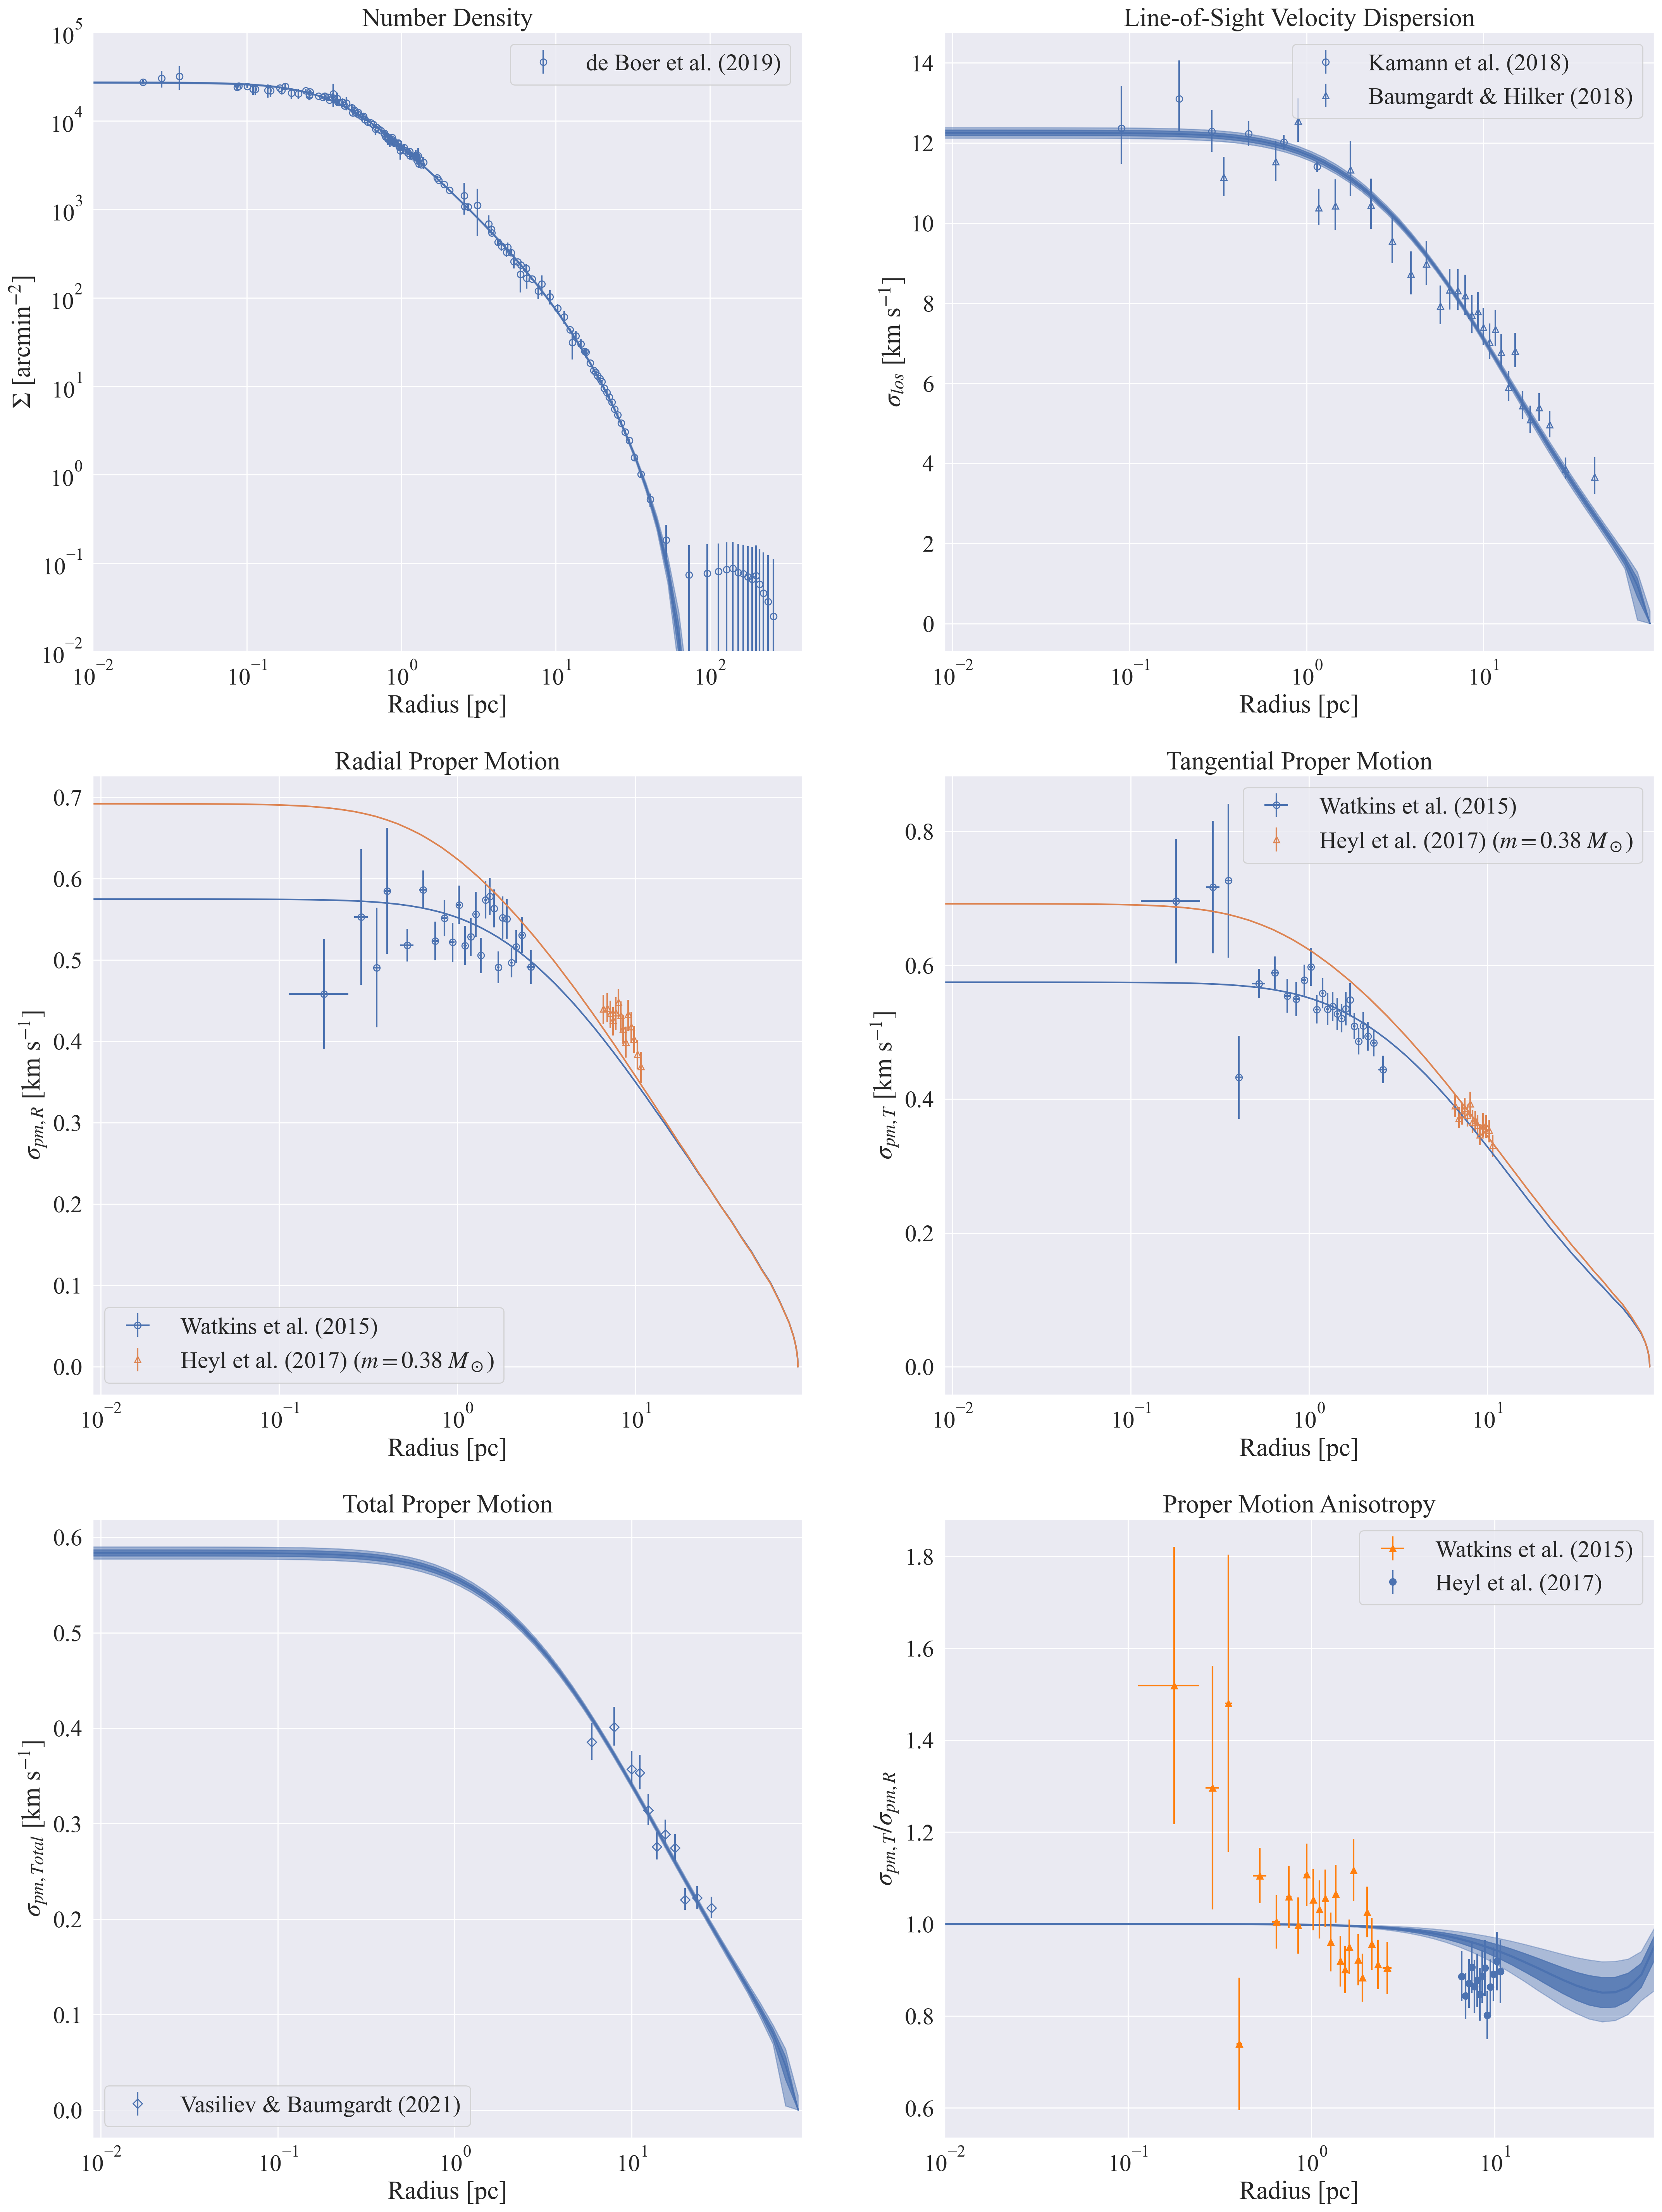
\includegraphics[width=0.9\textwidth]{figures/low_bin_model/obs_panel.png}
	\end{center}
	\caption{Observables}
	\label{fig:low_bin_model_obs_panel}
\end{figure}


\begin{figure}
	\begin{center}
		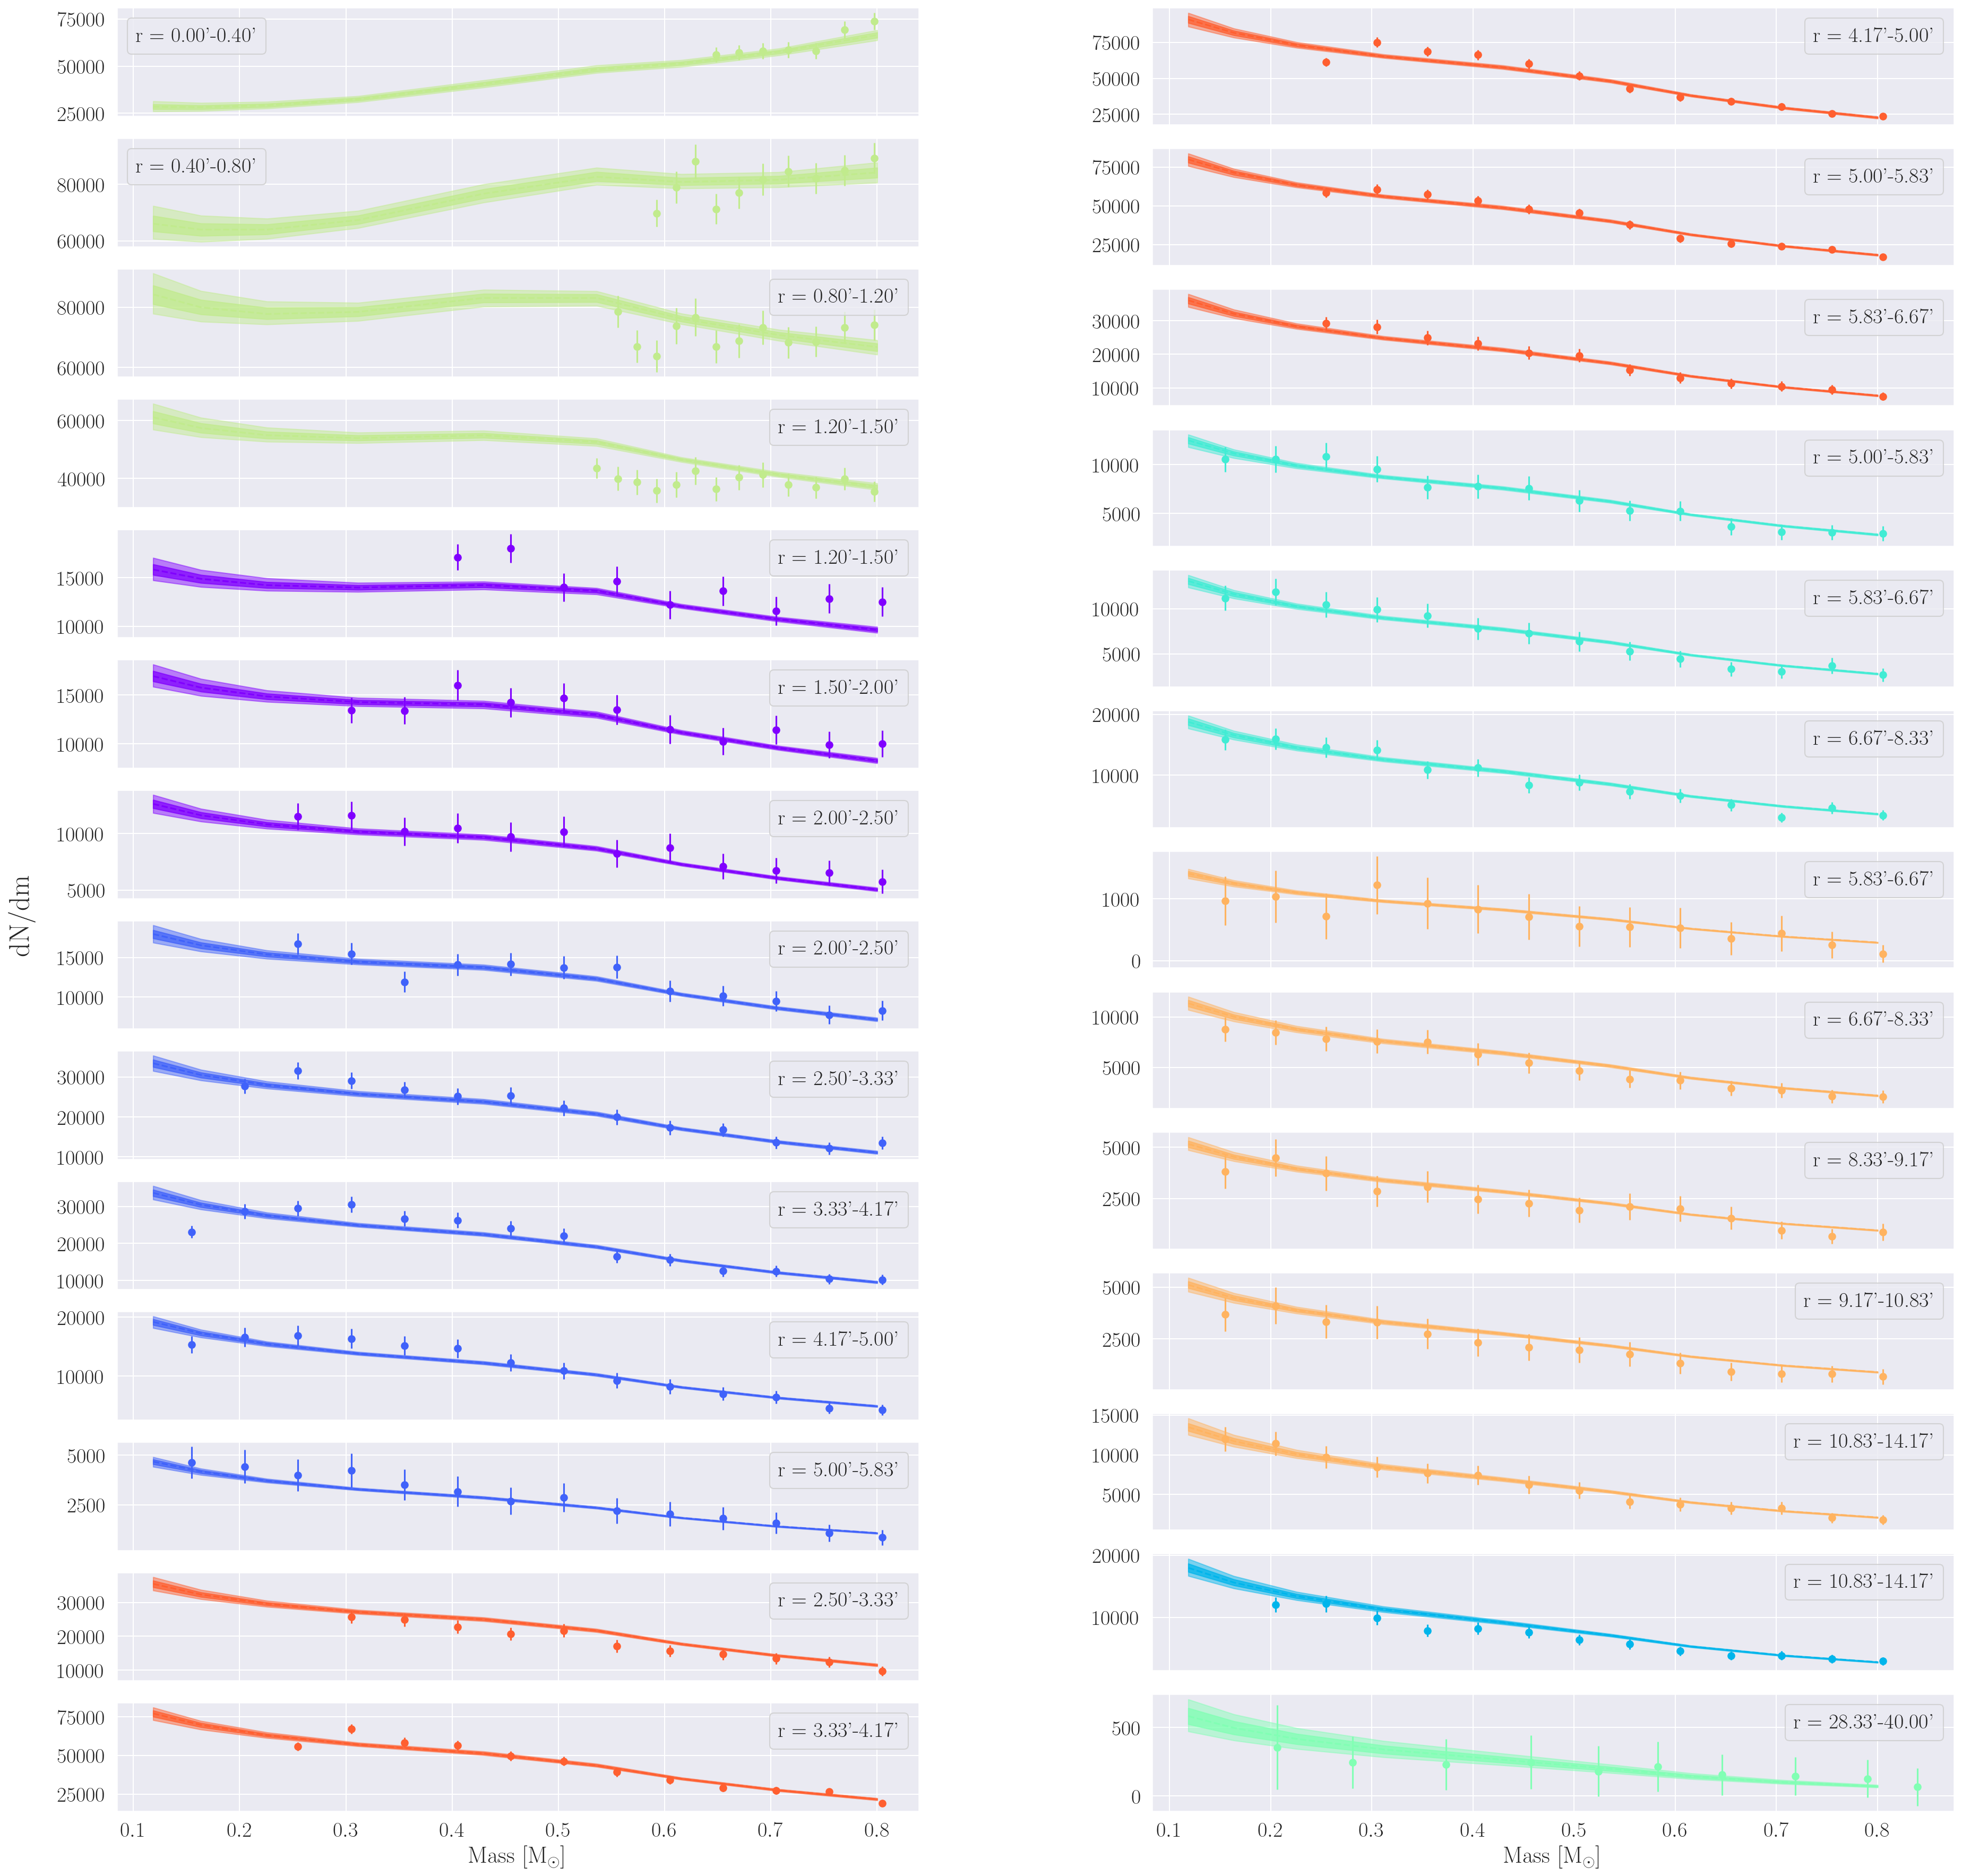
\includegraphics[width=\textwidth]{figures/low_bin_model/mass_fun.png}
	\end{center}
	\caption{Mass function}
	\label{fig:low_bin_model_mass_fun}
\end{figure}



\begin{figure}
	\centering
	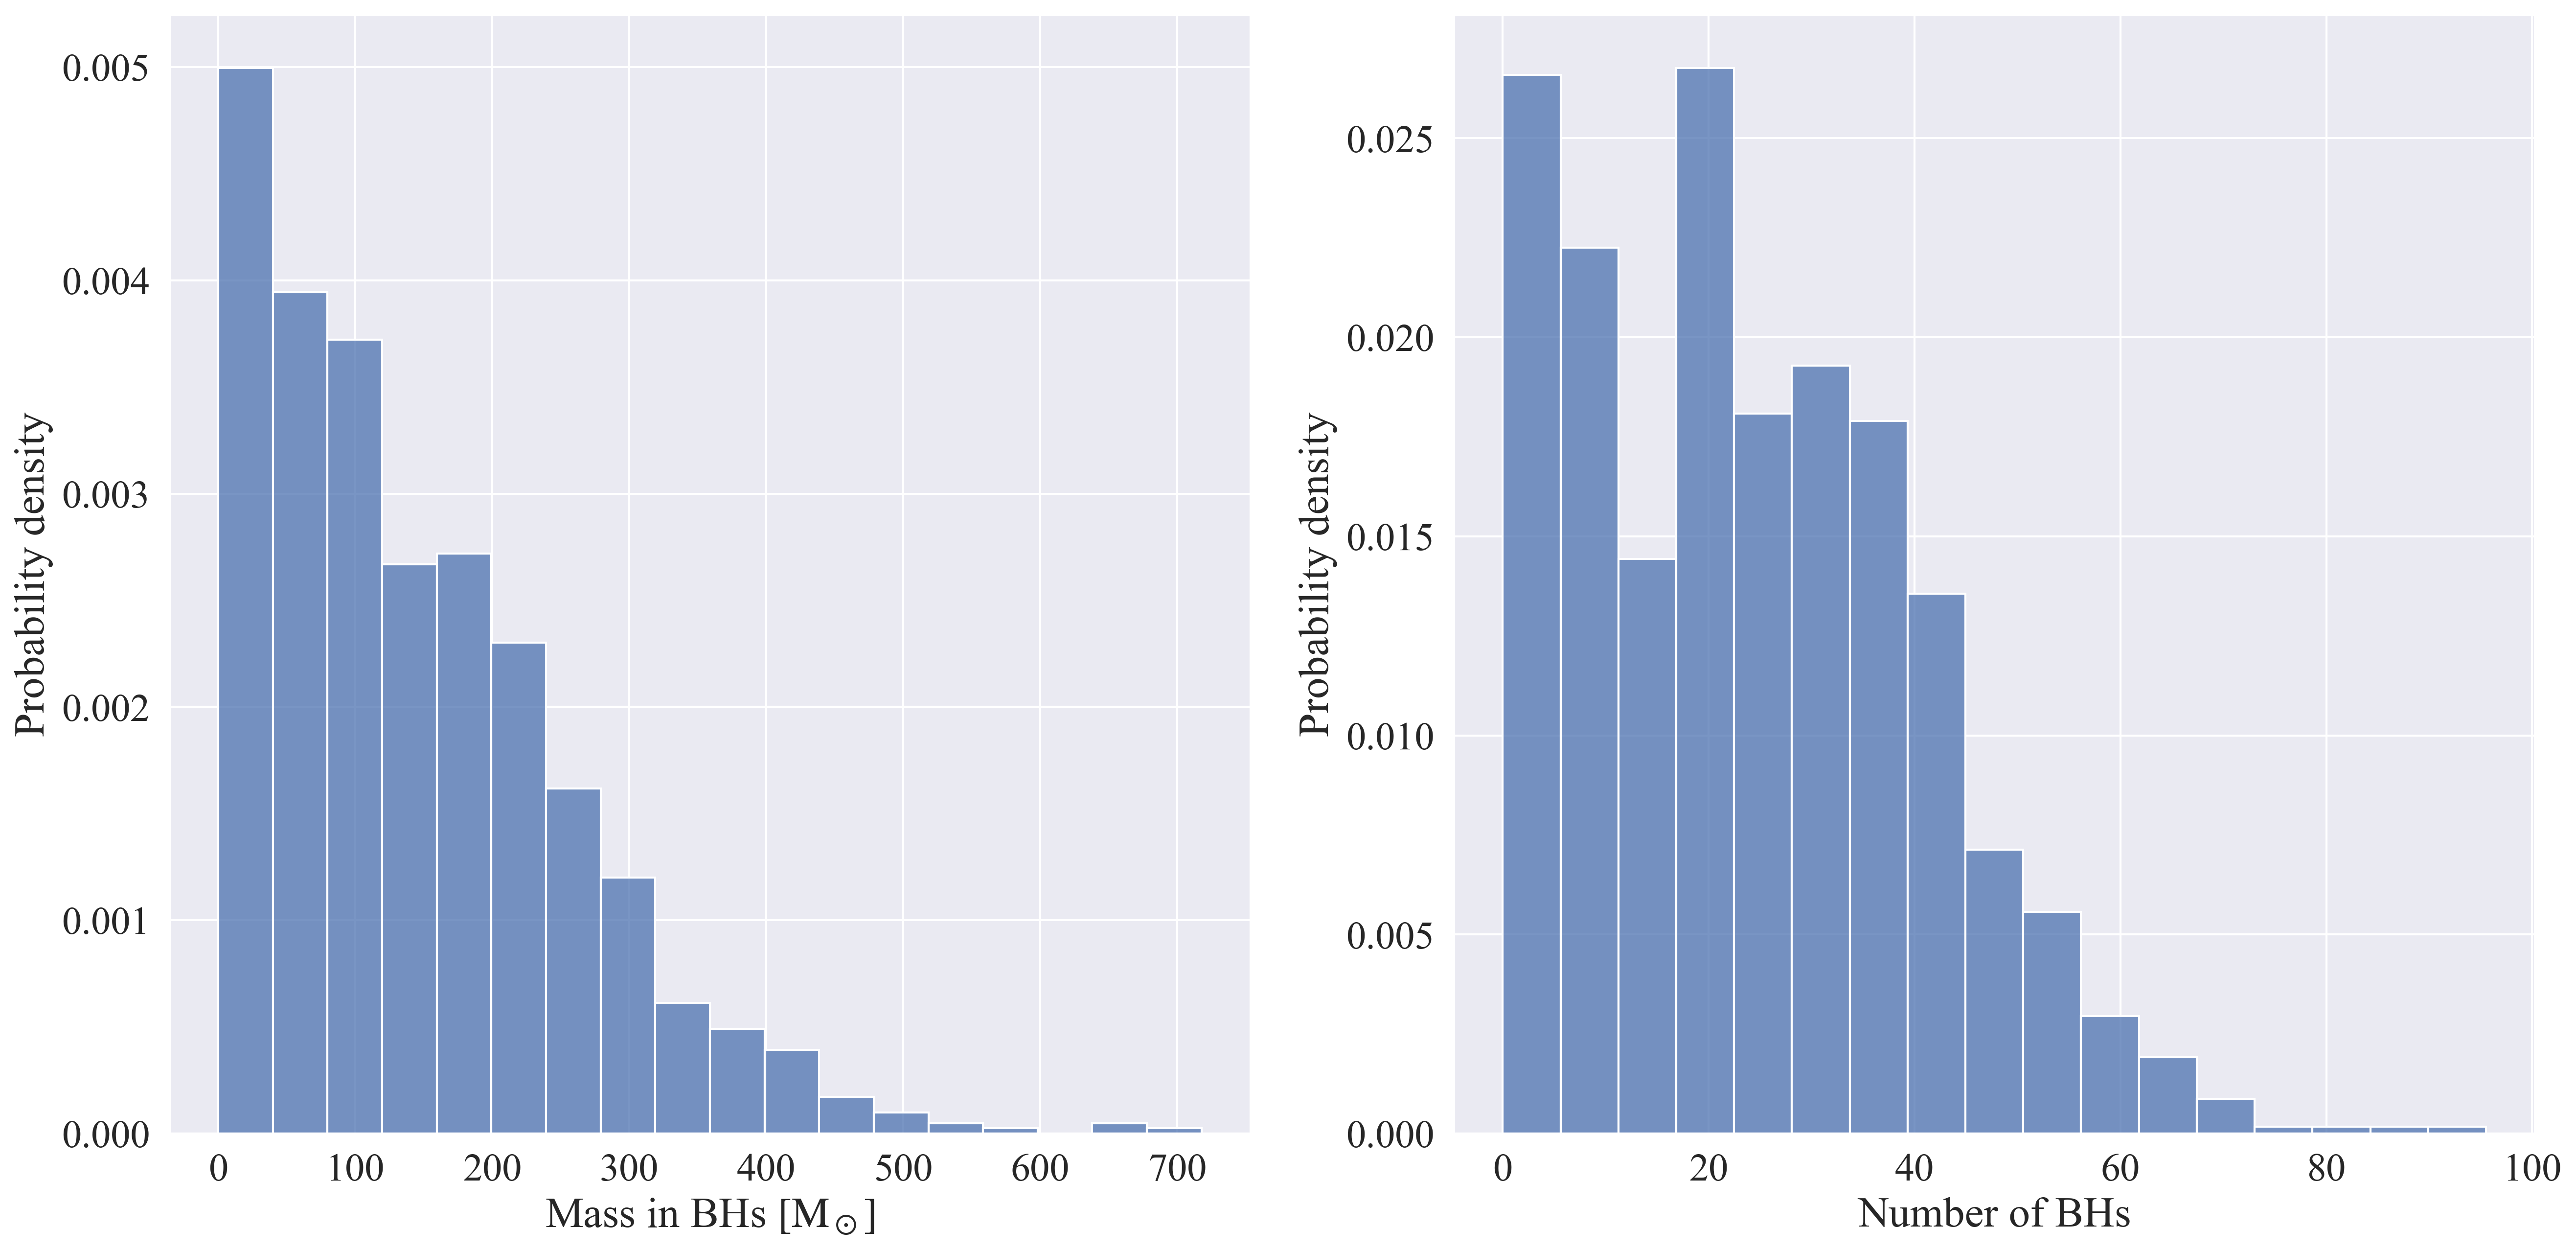
\includegraphics[width=0.8\textwidth]{figures/low_bin_model/BH_dists.png}
	\caption{BH distributions}
	\label{fig:low_bin_model_BH_dists}
\end{figure}





\subsection{High Binary Fraction}
\ps{Describe the results for the high binary fraction model.}

\ps{Figures with usual model quantities, also the binary mass histogram and the density profiles}



BH Mass: 80.697 solMass + 80.697 solMass - 120.702 solMass
BH Number: 12.162 + 12.162 - 13.332


\begin{figure}
	\centering
	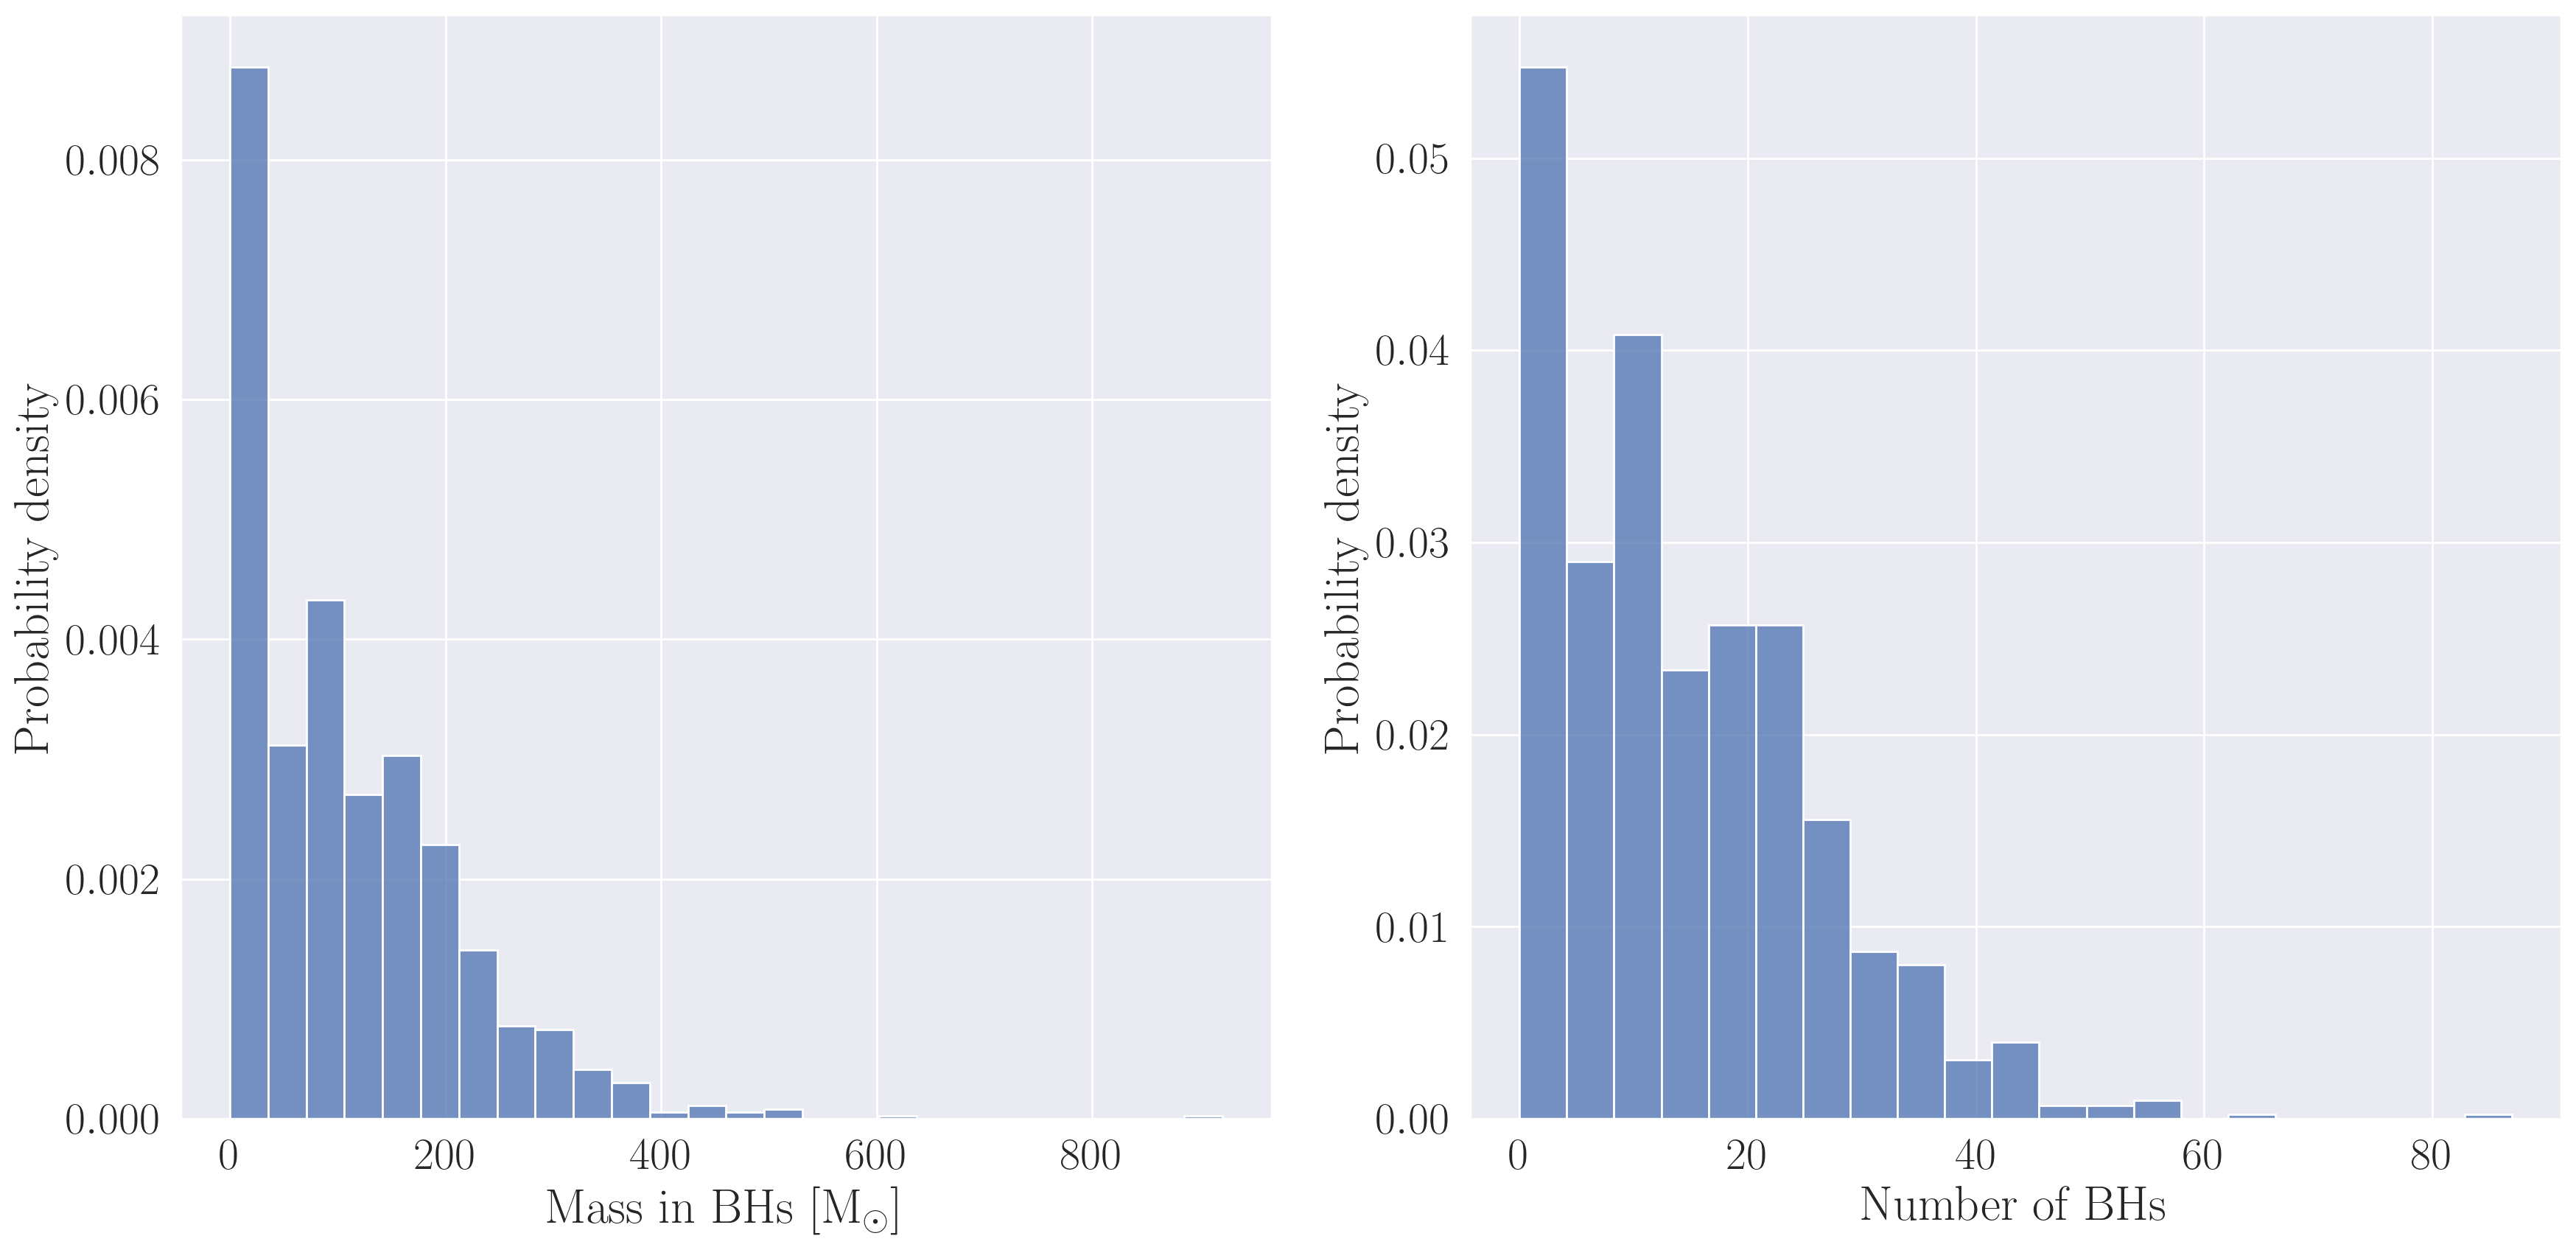
\includegraphics[width=0.8\textwidth]{figures/high_bin_model/BH_dists.png}
	\caption{BH distributions}
	\label{fig:high_bin_model_BH_dists}
\end{figure}

\section{Discussion}

\subsection{The effects of the binaries}

Generally mimic a small population of remnants?









\subsection{Conclusion}

\ps{Implications for past/future work}

\ps{Do binaries in df models actually matter?}








\subsection{Future Work}

We're only looking at binaries in main sequence stars. WD binaries are probably a bigger effect, but
we have no data at all to constrain those quantities, so we ignore them. Maybe looking at N-body or
MC models could give some useful constraints.

Would be nice to look at a cluster where we know there is a larger binary population (NGC3201)and
fit with and without binaries to see what the effects are.
\newpage


\chapter{Discussion}


\begin{table}
	\centering
	\caption{Best-fit parameters with $1\sigma$ credibility intervals for all sets of models.}
	\begin{tabular}{l l l l}

		\hline
		Parameter                 & Value                                                                    \\
		\hline
		$f_b$                     & $0\%$                  & $2\%$                  & $10\%$                 \\
		$W_0$                  & $6.26^{+0.10}_{-0.10}$ & $6.28^{+0.10}_{-0.10}$ & $6.36^{+0.09}_{-0.09}$ \\
		$M/10^6 \mathrm{M}_\odot$ & $0.88^{+0.01}_{-0.01}$ & $0.89^{+0.01}_{-0.01}$ & $0.89^{+0.01}_{-0.01}$ \\
		$r_h / pc$                & $6.72^{+0.06}_{-0.06}$ & $6.74^{+0.06}_{-0.06}$ & $6.77^{+0.06}_{-0.06}$ \\
		$\log_{10}{r_a / pc}$     & $1.51^{+0.07}_{-0.05}$ & $1.50^{+0.06}_{-0.05}$ & $1.48^{+0.06}_{-0.05}$ \\
		$g$                       & $1.37^{+0.06}_{-0.06}$ & $1.36^{+0.06}_{-0.06}$ & $1.34^{+0.06}_{-0.06}$ \\
		$\delta$                  & $0.43^{+0.02}_{-0.02}$ & $0.43^{+0.02}_{-0.02}$ & $0.41^{+0.01}_{-0.01}$ \\
		$s^2$                     & $0.01^{+0.01}_{-0.00}$ & $0.01^{+0.01}_{-0.00}$ & $0.01^{+0.01}_{-0.00}$ \\
		$F$                       & $3.26^{+0.13}_{-0.12}$ & $3.24^{+0.13}_{-0.12}$ & $3.16^{+0.13}_{-0.12}$ \\
		$\alpha_1$                & $0.35^{+0.02}_{-0.02}$ & $0.37^{+0.02}_{-0.02}$ & $0.45^{+0.02}_{-0.02}$ \\
		$\alpha_2$                & $1.46^{+0.05}_{-0.05}$ & $1.47^{+0.05}_{-0.05}$ & $1.53^{+0.05}_{-0.04}$ \\
		$\alpha_3$                & $2.13^{+0.04}_{-0.03}$ & $2.18^{+0.04}_{-0.04}$ & $2.46^{+0.05}_{-0.05}$ \\
		$BH_{ret} (\%)$           & $0.07^{+0.06}_{-0.05}$ & $0.08^{+0.09}_{-0.05}$ & $0.17^{+0.18}_{-0.12}$ \\
		$d$                       & $4.42^{+0.02}_{-0.02}$ & $4.42^{+0.02}_{-0.02}$ & $4.43^{+0.02}_{-0.02}$ \\
		\hline
	\end{tabular}
	\label{tab:parameters_all}
\end{table}







In each set of models, all observables are very well reproduced, showing the flexibility of the
\code{LIMEPY} models. Due to this flexibility, it is unlikely that with current observations we
would be able to infer anything about the binary population of a cluster using this technique.
Instead, this method should be used in cases where there are existing estimates of the binary
population within a cluster in order to add a realistic binary component to \code{LIMEPY} models



\section{The Effects of the Binaries}


Table \ref{tab:parameters_all} shows the recovered parameters for each set of models. We can see a
clear agreement in the recovered values of the parameters which affect the overall structure of the
cluster. In particular, the total cluster mass, half-mass radius, anisotropy radius, truncation
parameter, degree of mass segregation and distance are all either identical or within $1\sigma$ of
each other for all three sets of models.



The most striking change in model parameters are the values pertaining to the mass function, in
particular, the $\alpha_3$ parameter which controls the slope of the high-mass mass function (above
$1.0 \ \mathrm{M}_\odot$). In the case with a $10\%$ binary fraction, this parameter is much larger
than in the other two cases showing that the abundance of binary stars reduces the need for high-mass
stars and remnants.

We can see that there is still some need for black holes in some of the models with a high binary fraction
as the $BH_{ret}$ parameter is much larger in the model with many binaries, this means that even
though the initial mass function produces many fewer black holes, more of these black holes need to
be retained throughout the evolution of the cluster.

Table \ref{tab:BH_contents} and Figure \ref{fig:BH_KDEs} show the distribution of BHs for each set
of models. We can see a clear decrease in the inferred black hole content as we add more binaries
though we also note that all three sets of models are consistent with zero black holes within their
$2\sigma$ intervals. This effect of binaries reducing the need for black holes was also found by
\citet{Mann2019} (see also associated erratum \citealt{Mann2020}) when they modelled the central
kinematics of 47\,Tuc. This effect is due to the high-mass binary systems which have mass-segregated
to the central regions of the cluster contributing to the central mass distribution in a similar way
to heavy stellar remnants. Through this process, fewer black holes are needed to create the observed
central velocity dispersion. This effect is particularly clear in Figure \ref{fig:mass_enc_comp}
where we examine the enclosed mass profiles of remnants and binaries for the no-binary and
high-binary cases.



\begin{figure}
	\centering
	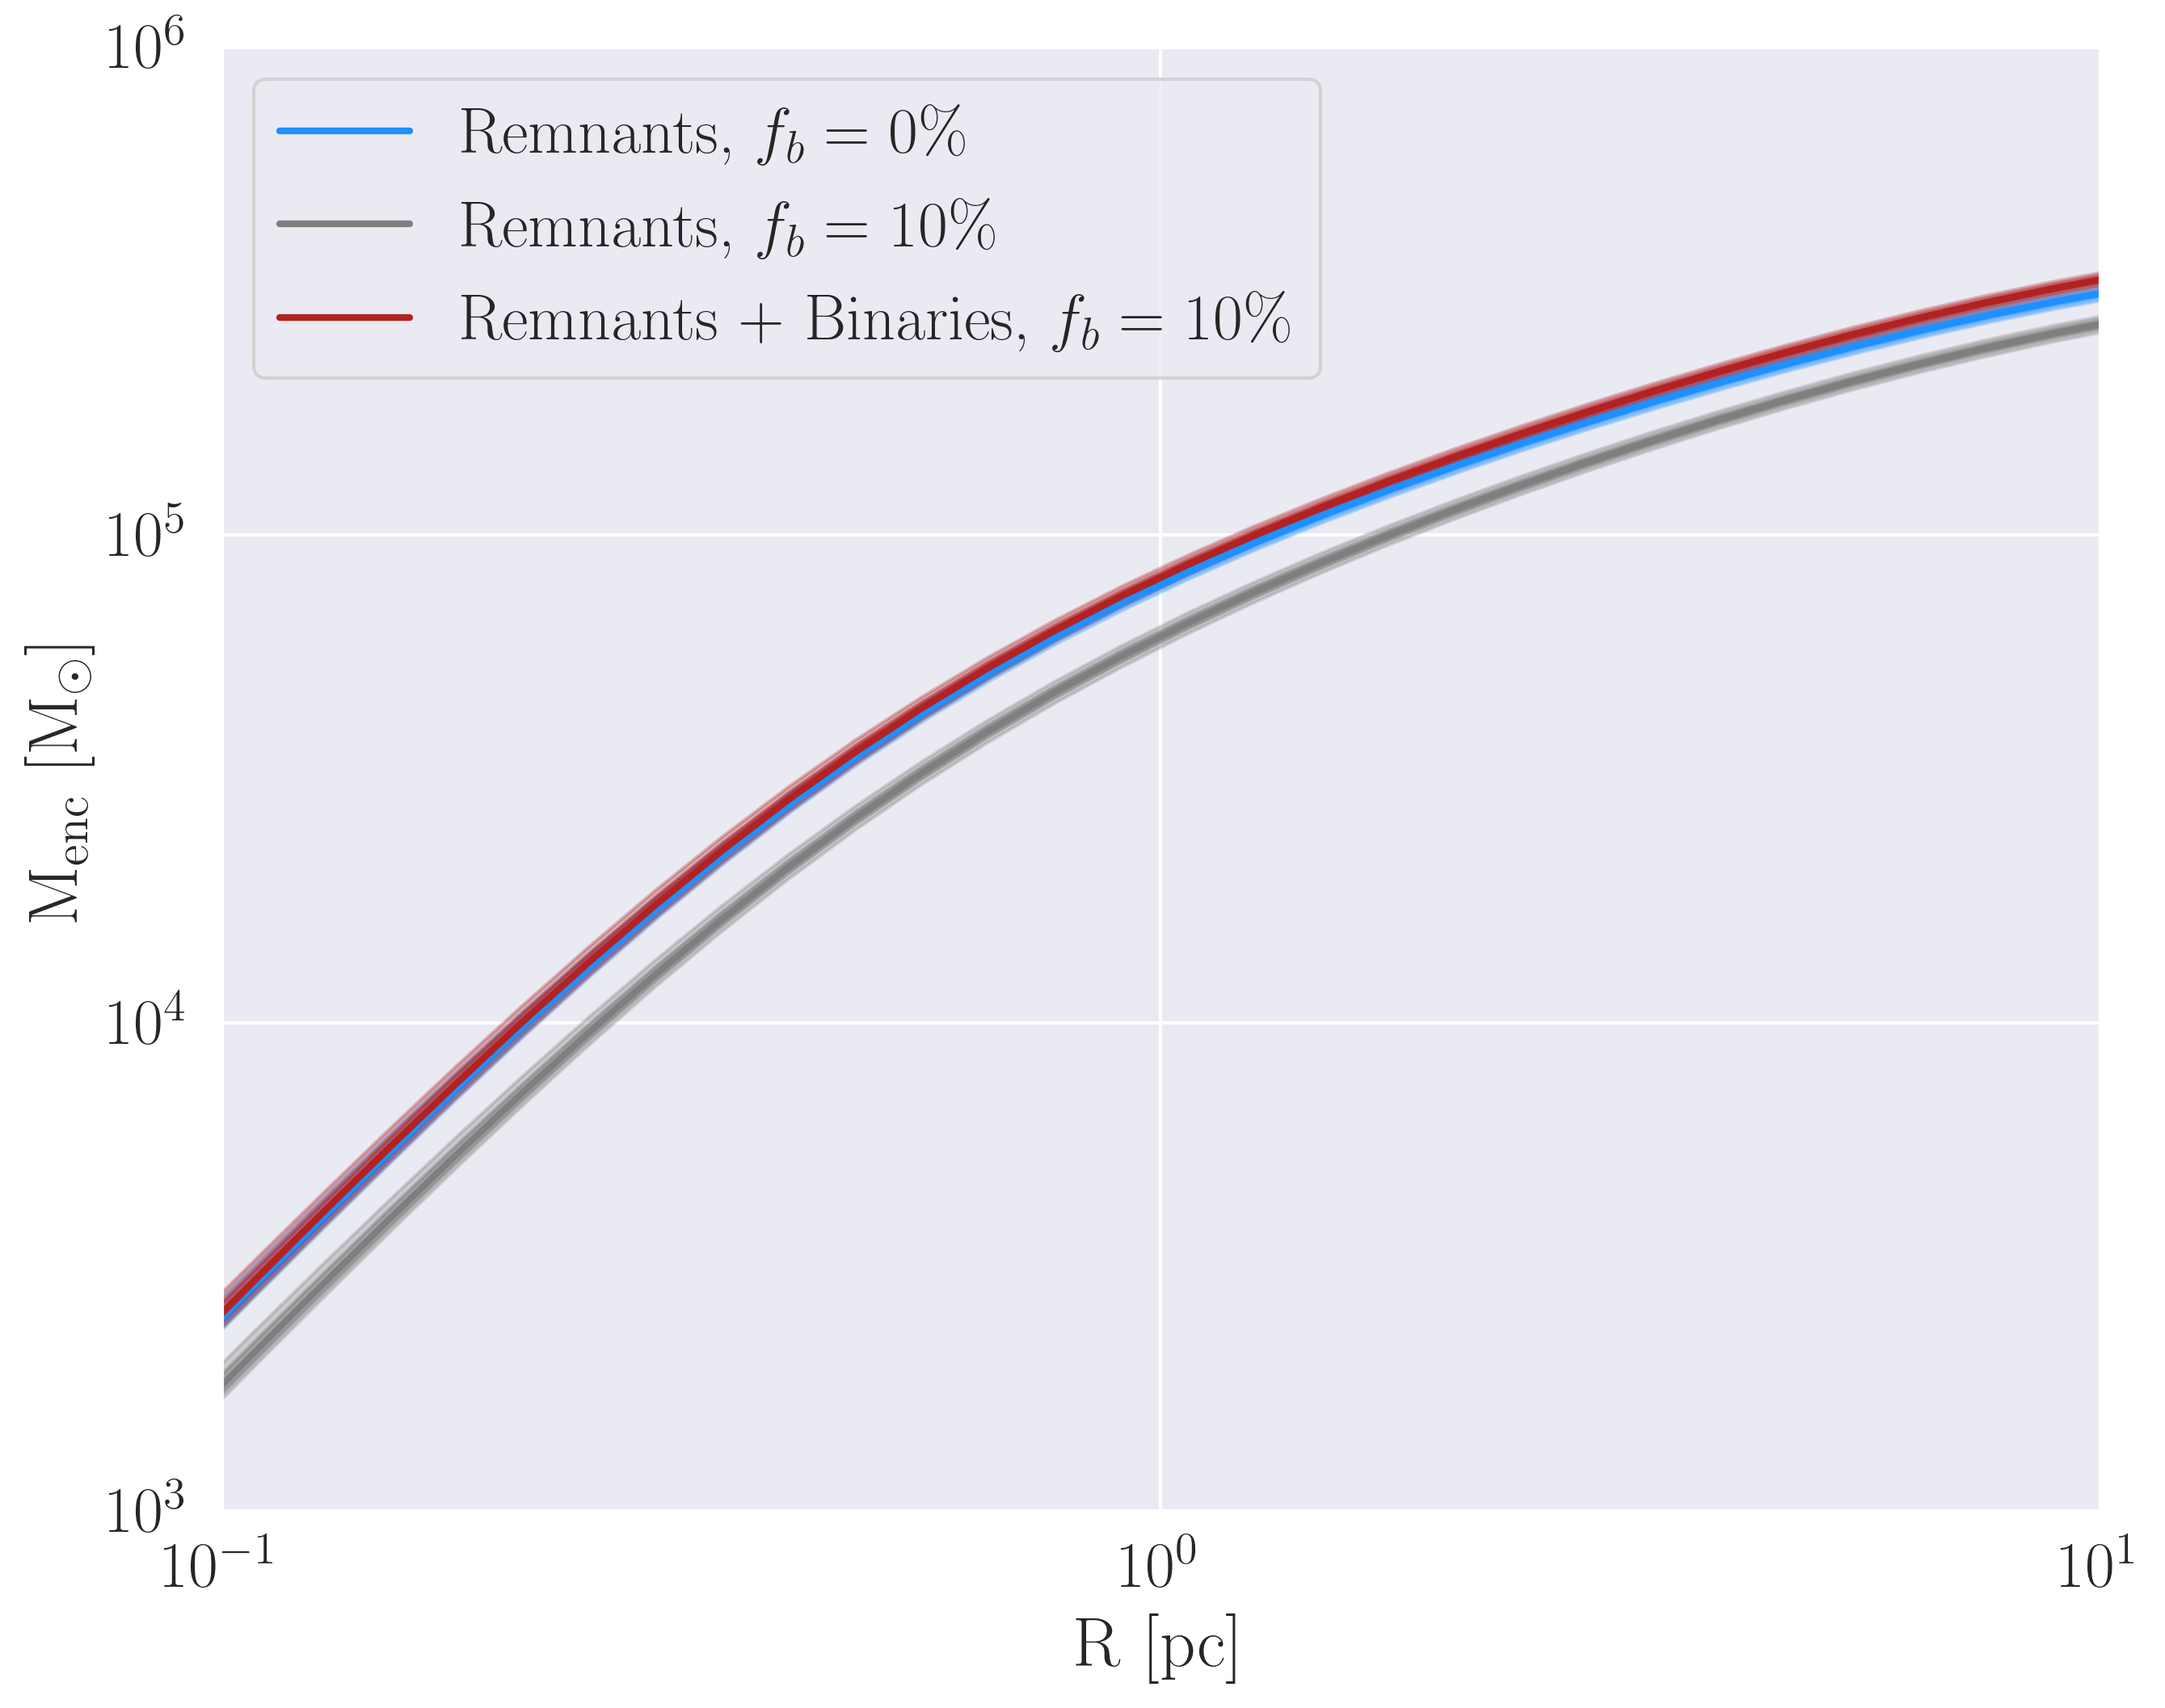
\includegraphics[width=0.8\textwidth]{figures/mass_enc_comp.png}
	\caption{Enclosed mass profiles for the stellar remnants in the $f_b =0\%$ model and the
		remnants and remnants plus binaries in the $f_b =10\%$ model. The two remnant
		profiles are very different between the $f_b = 0\%$ and $f_b = 10\%$ cases which
		mirrors the lower black hole content. The most interesting part of these profiles is
		the fact that when the \emph{binaries} are added to the remnants the enclosed mass
		profiles match very well. This demonstrates very clearly that the binaries are
		filling the same role as the heavy remnants in the central regions of the cluster
		and explains why adding binaries reduces the need for black holes in the models.}
	\label{fig:mass_enc_comp}
\end{figure}


% Table comparing bh content in each set of models
\begin{table}
	\centering
	\caption{Black hole content in each set of models}
	\begin{tabular}{c c c}
		\hline
		Binary Fraction $(\%)$ & Mass in BHs                         & Number of BHs    \\
		\hline
		0                      & $136^{+108}_{-91} \mathrm{M}_\odot$ & $26^{+15}_{-15}$ \\
		2                      & $114^{+144}_{-79} \mathrm{M}_\odot$ & $22^{+19}_{-13}$ \\
		10                     & $81 ^{+121}_{-81} \mathrm{M}_\odot$ & $12^{+13}_{-12}$ \\
		\hline
	\end{tabular}
	\label{tab:BH_contents}
\end{table}


\begin{figure}
	\centering
	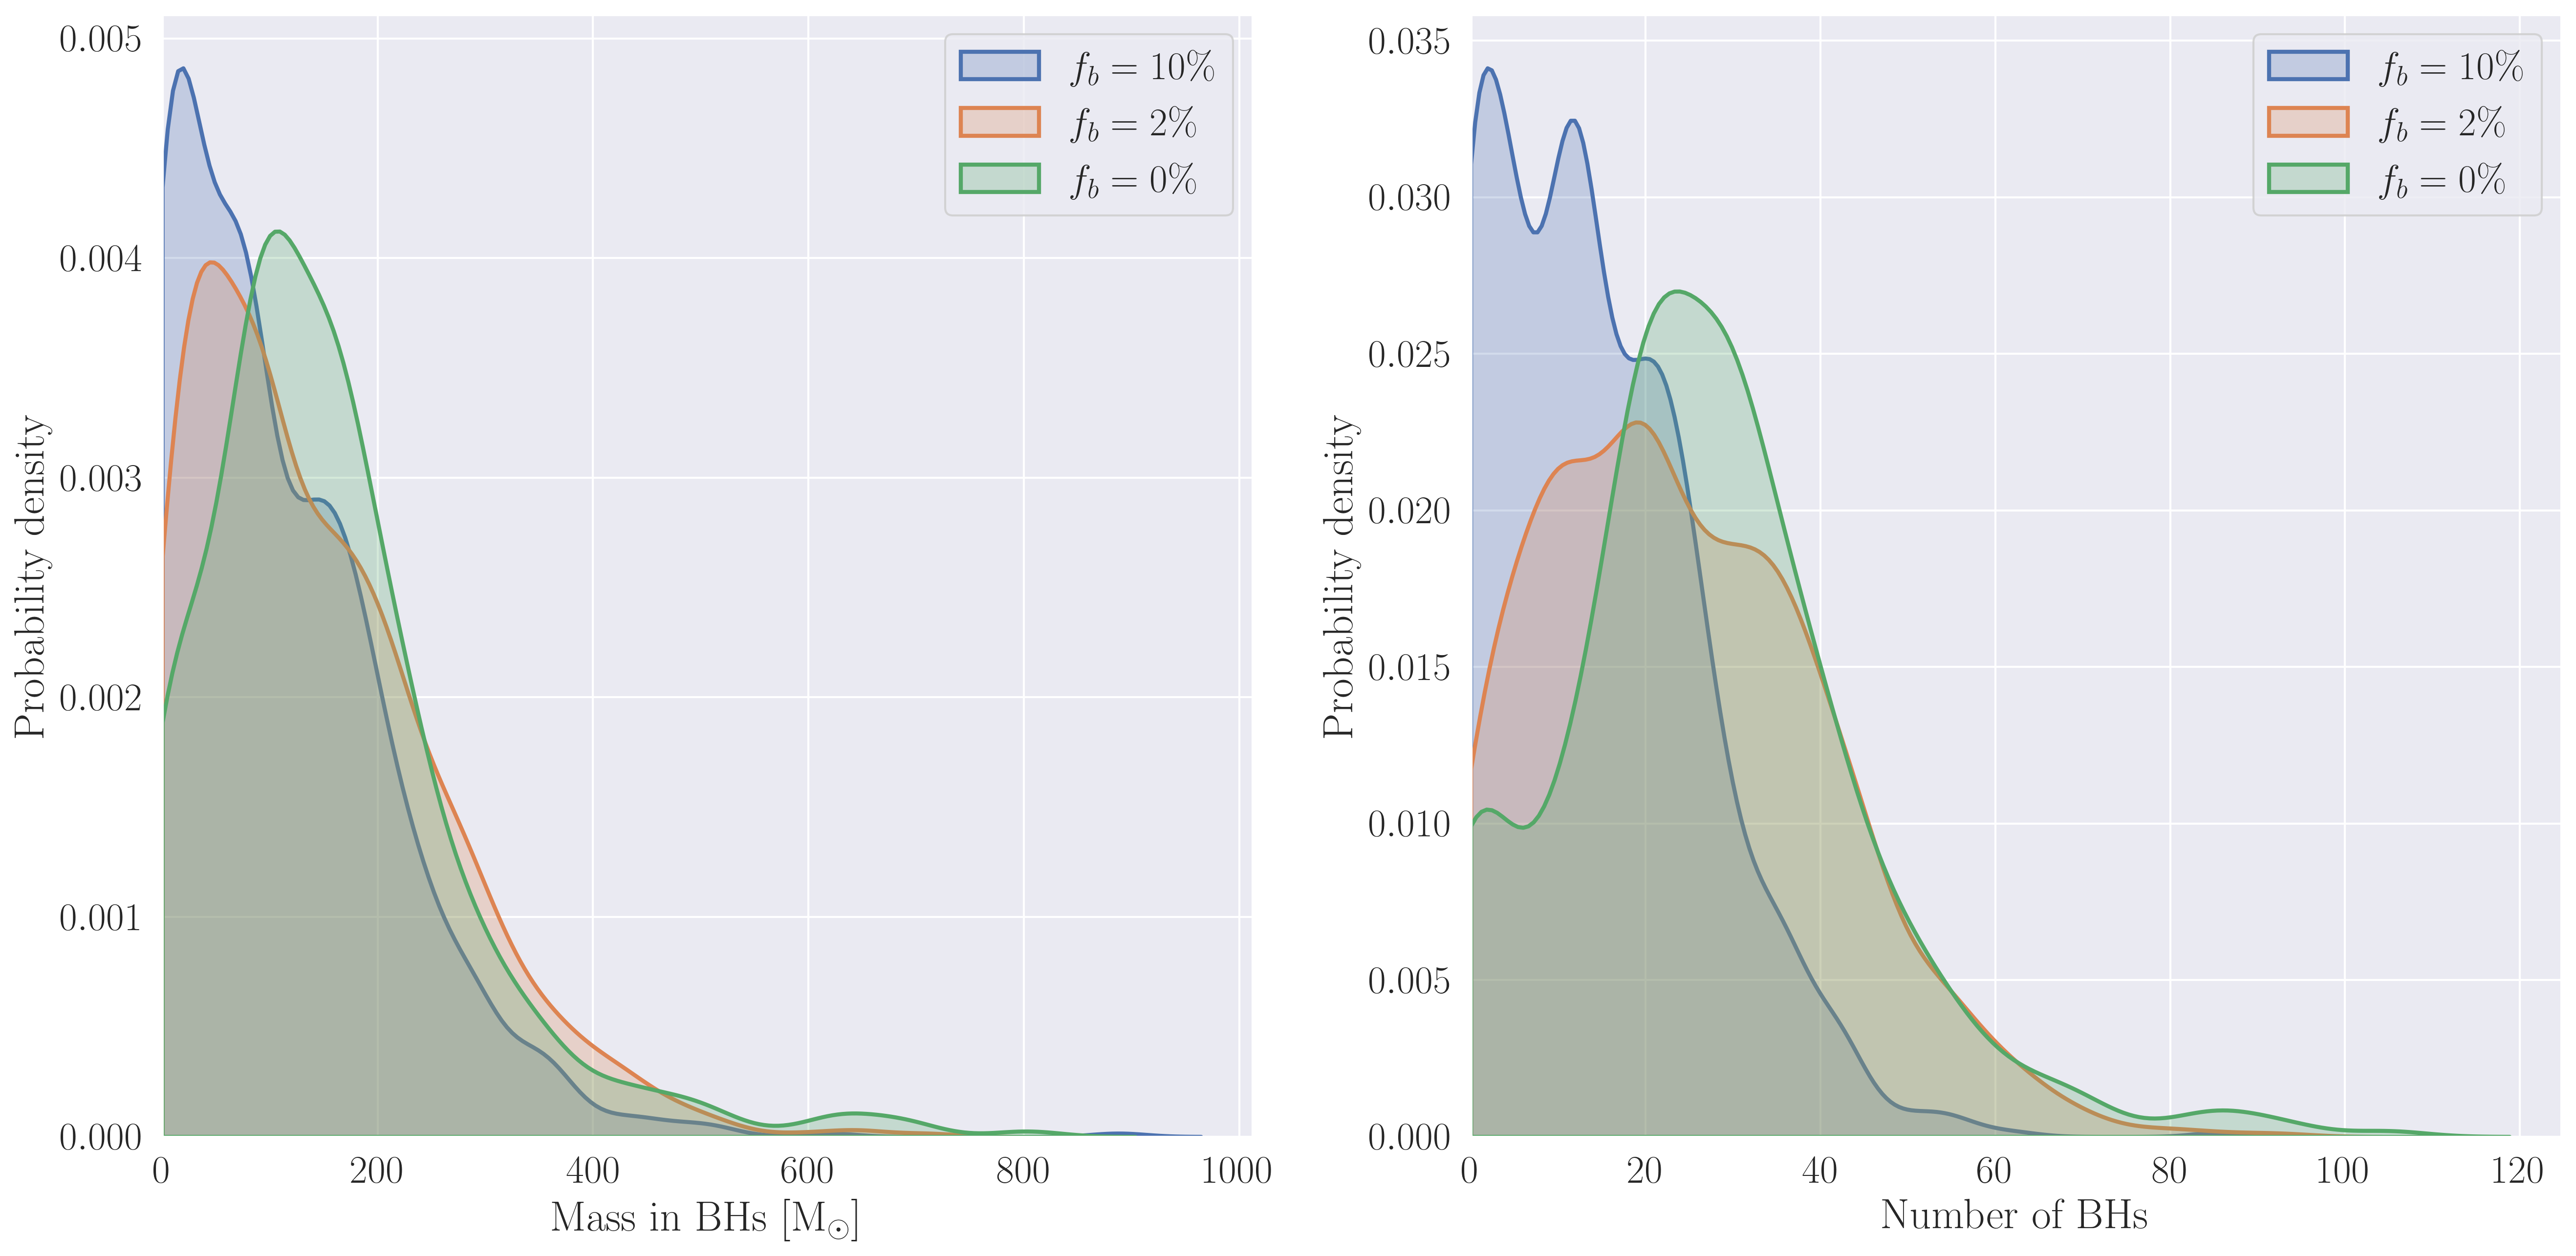
\includegraphics[width=\textwidth]{figures/BH_KDEs.png}
	\caption{Distribution of mass and number of BHs in each set of models. Distributions are
		represented by a Gaussian kernel density estimator of the discrete values for easier visual
		comparison.}
	\label{fig:BH_KDEs}
\end{figure}

When we examine the density profiles for the models with a binary fraction of $10\%$ (see Figure
\ref{fig:highbin_model_densities}), we can see that the binary stars are indeed more centrally
concentrated than typical main-sequence stars as predicted and in the central regions, make up
almost all the main-sequence contribution, while they contribute more than the neutron stars at all
radii.



\begin{figure}
	\centering
	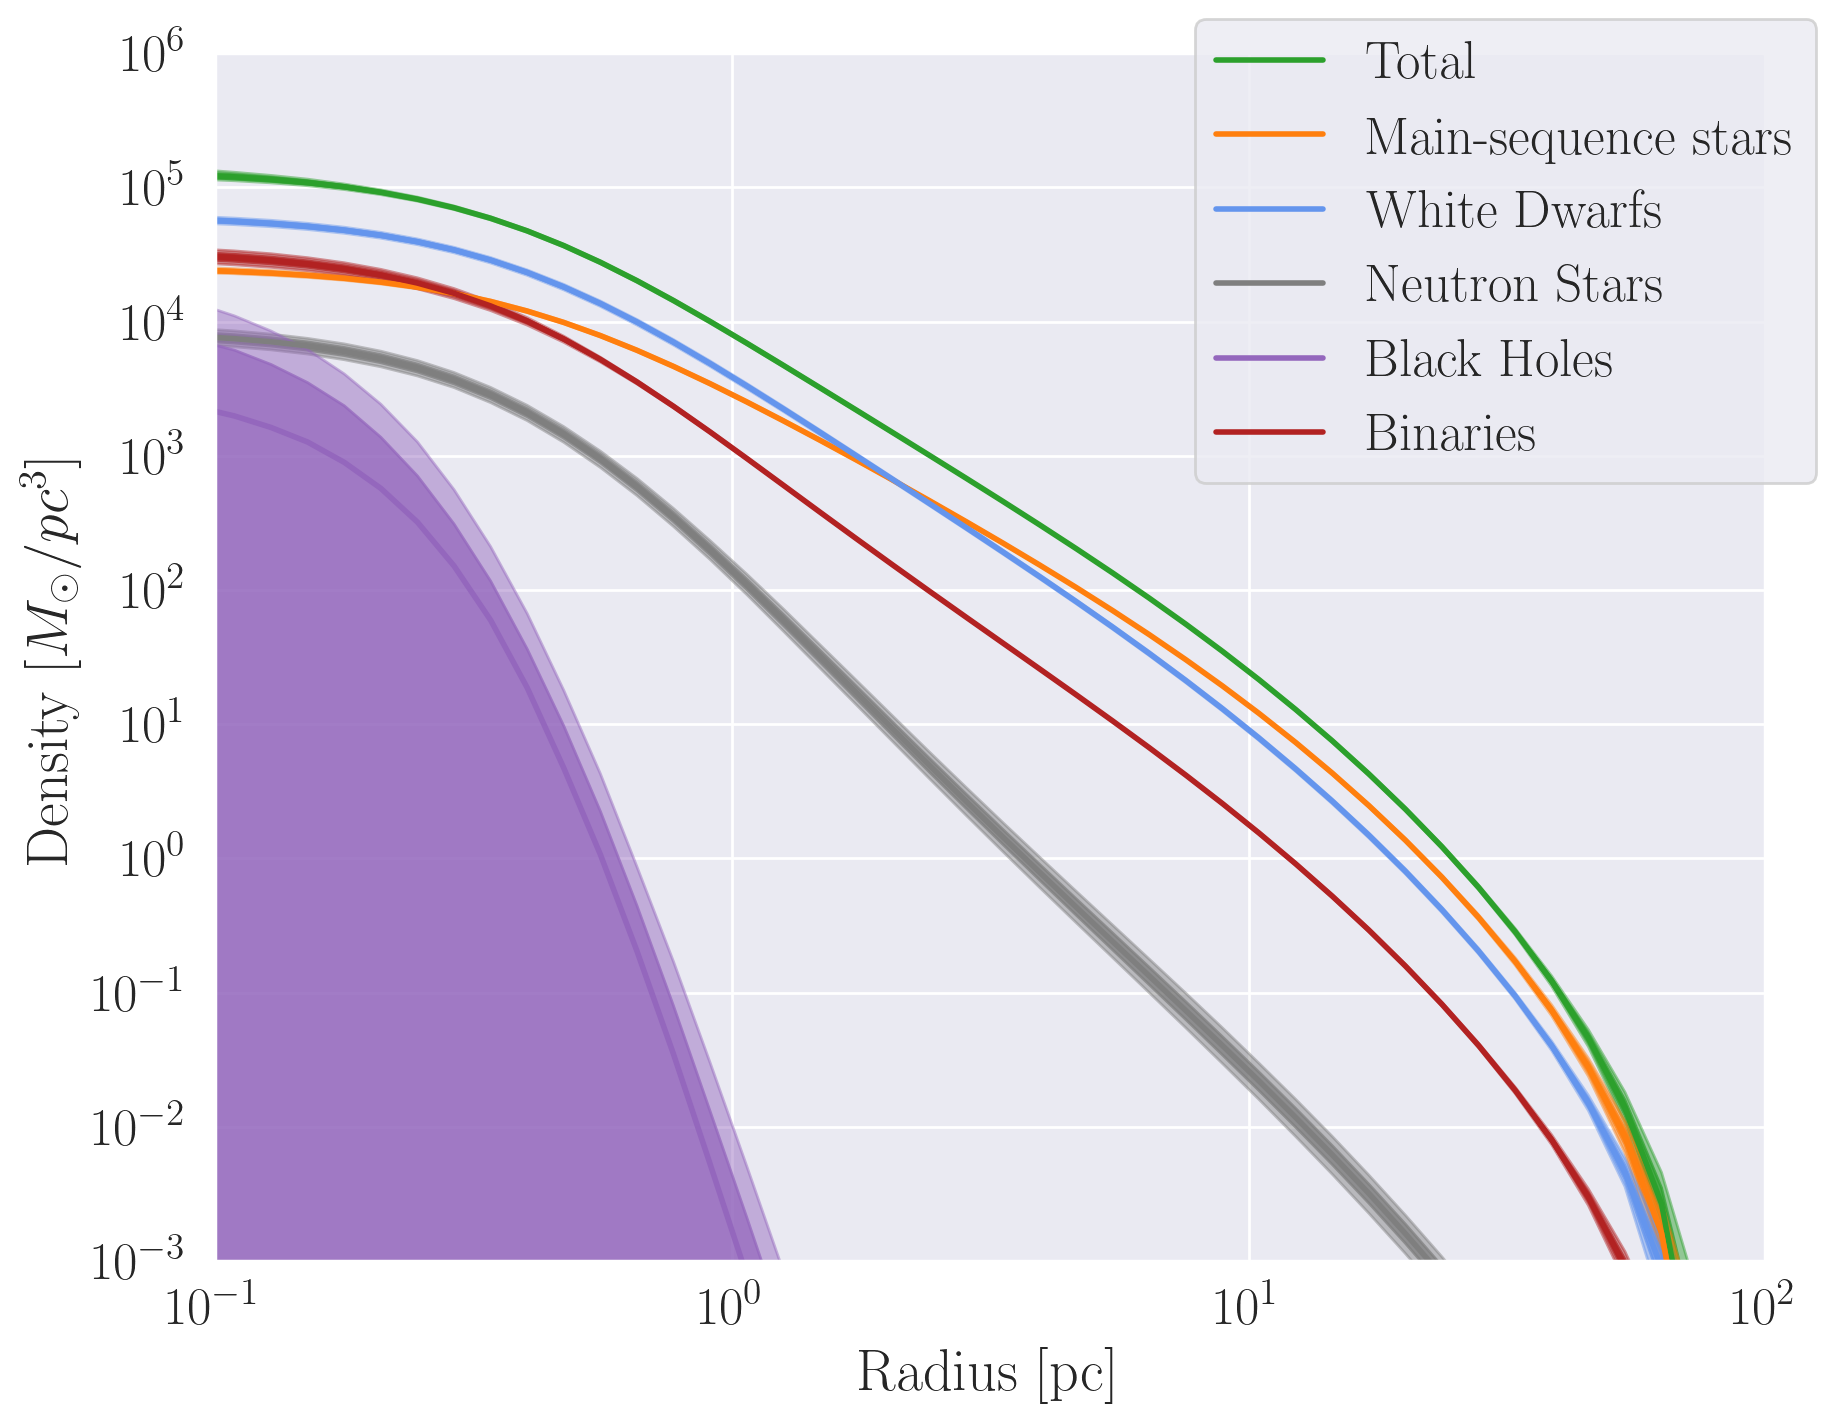
\includegraphics[width=0.8\textwidth]{figures/high_bin_model/density.png}
	\caption{Mass density profiles for the models with a binary fraction of $10\%$}
	\label{fig:highbin_model_densities}
\end{figure}


\newpage


\appendix
\chapter{Appendix}


%---> BIBLIOGRAPHY <---------------------------------------------------------------------

\begin{singlespace}
    \bibliography{research}
\end{singlespace}
\end{document}
